\documentclass[12pt]{article}

\usepackage{amsmath,amsthm,amssymb,amsfonts}
\usepackage{mathtext}
\usepackage{makeidx}
\usepackage[T2A]{fontenc}
\usepackage[utf8]{inputenc}
\usepackage[russian]{babel}
\usepackage[pdftex]{graphicx}
\graphicspath{{pictures/}}
\DeclareGraphicsExtensions{.pdf,.png,.jpg}
\usepackage[left=1cm,right=1cm,top=1cm,bottom=1cm,bindingoffset=0cm]{geometry}
\usepackage{cmap}

%\hoffset=-3cm
%\textwidth=18cm
%\voffset=-3cm
%\textheight=26cm

\begin{document}
%\fontsize{15}{25pt}\selectfont

\section{Комбинаторные правила произведения и суммы. Число выборок объема k из n элементов. }

\subsection{Правило произведенеия}
	Если $a \in A$ можно выбрать $n$ способами и для каждого такого выбора
	$b \in B$ можем выбрать $m$ способами, то пару $ab$ мы можем выбрать $n\cdot m$ способами.\\
	$| A_1 \times \dotsb \times A_n| = |A_1| \times \dotsb \times |A_n|$

\subsection{Правило суммы}
	Если элемент $a \in A$ может быть выбран $n$ способами и независимо, а элемент $b \in B$ может быть выбран m способами, то выбор "$a$ или $b$" может быть осуществлён $n + m$ способами.\\
	$\forall$ разбиения конечного множества A = $A_1 \sqcup \dotsb \sqcup A_n \newline$ 
	$|A| = |A_1| + \dotsb + |A_n|$

\subsection{Число выборок объема k из n элементов}
\subsubsection{Упорядоченная выборка объема k из n элементов с повторениями (число кортежей)}
	$\widetilde{A}_n^k = n^k$

\subsubsection{Упорядоченная выборка объема k из n элементов без повторений (число k-размещений)}
	$[n]_k = n(n - 1)\dotsb(n - k + 1) = \frac{n!}{(n-k)!}$\\
	\textbf{Доказательство:}\\
	Индукция по k:\\
	$k = 1$: $[n]_1 = n$\\
	$k > 1$: $[n]_k = [n]_{k-1}(n-k+1)$\\
	\qedsymbol

\subsubsection{Неупорядоченные выборки объема k из n элементов без повторений (сочетания)}
	$\forall$ $n,k$ $0 \leqslant k \leqslant n$\\
	$\binom{n}{k} = C_n^k = \frac{[n]_k}{k!} = \frac{n!}{k!(n-k)!}$\\\\
	\textbf{Доказательство:}\\
	Индукция по $n$\\
	$n = 1$: $\binom{1}{0} = 1$; $\binom{1}{1} = 1$\\
	$n \geqslant 2$:\\
	Если $k = n$, то $\binom{n}{n} = 1 = \frac{n!}{n!\cdot0!}$\\
	Если $k < n$, то\\
	$\binom{n}{k} = \binom{n-1}{k} + \binom{n-1}{k-1} = \frac{(n-1)!}{k!(n-k-1)!} + \frac{(n-1)!}{(k-1)!(n-k)!} = \frac{(n-1)!(n-k+k)}{k!(n-k)!} = \frac{n!}{k!(n-k)!}\\$
	\qedsymbol\\
\subsubsection{Неупорядоченные выборки объема k из n элементов с повторениями (число мультимножеств)}
	$\widehat{C}^m_n = C^{n-1}_{n+m-1} = C^{m}_{n+m-1}$\\
	\textbf{Доказательство:}\\
	<$\alpha_1,\dotsc\alpha_n$> задаёт наше m-сочетание с повторениями\\
	Сопоставим ему двоичный кортеж\\
	$(\underbrace{0,\dotsc,0}_{\alpha_1},1,\underbrace{0,\dotsc,0}_{\alpha_2},1,\dotsc,1,\underbrace{0,\dotsc,0}_{\alpha_n})$\\
	Знаем, что $\displaystyle\sum_{i=1}^{n}\alpha_i = m$ $\Rightarrow$ длина кортежа $m + n - 1$ и в нём $n-1$ единица. Таких кортежей $C^{n-1}_{n+m-1}$\\
	\qedsymbol

\section{Число выборок объема k из n элементов. Комбинаторные тождества. Бином Ньютона.}
\subsection{Число выборок объема k из n элементов.}
	См. пункт 1.3
\subsection{Комбинаторные тождества}
\subsubsection{Тождество Паскаля}
	$\forall n,k$ $1 \leqslant k < n$\\
	$\binom{n}{k} = \binom{n-1}{k} + \binom{n-1}{k-1}$\\
	\textbf{Доказательство:}\\
	M — все k-подмножества n-множества\\
	$|M| = \binom{n}{k}$\\
	$M_1 \subseteq M$  — не попал элемент a\\
	$M_2 \subseteq M$  — попал элемент a\\
	$\Downarrow$\\
	$M = M_1 \sqcup M_2 \Rightarrow |M| = |M_1| + |M_2| = \binom{n-1}{k} + \binom{n-1}{k-1}$\\
	\qedsymbol

\subsubsection{}
	$\binom{n}{k} = \binom{n}{n-k}$\\
	\textbf{Доказательство:}\\
	$\binom{n}{n-k} = \frac{n!}{(n-k)!(n-(n-k))!} = \frac{n!}{(n-k)!k!} = \binom{n}{k}$\\
	\qedsymbol

\subsection{Бином Ньютона}
	$\forall n \in \mathbb N$\\
	$(a+b)^n = \displaystyle\sum_{k=0}^n\binom{n}{k}a^kb^{n-k}$\\
	\textbf{Доказательство:}\\
	$(a+b)^n = (a+b)(a+b)\dotsm(a+b) = \displaystyle\sum_{k=0}^n\binom{n}{k}a^kb^{n-k}$\\
	\qedsymbol

\subsection{Обобщение бинома Ньютона}
	$(x_1+\dotsb+x_k)^n = \displaystyle\sum_{\alpha_1,\dotsc,\alpha_k ; \alpha_i \geqslant 0 ; \alpha_1+\dotsb+\alpha_k = n} P_n(\alpha_1\dotsc\alpha_k)x_1^{\alpha_1}\dotsm x_k^{\alpha_k}$\\
	$P_n(\alpha_1\dotsc\alpha_k)$ — полиномиальный коэффициент\\
	\textbf{Доказательство:}\\
	Упражнение\\
	\qedsymbol

\section{Мультимножества, их спецификации. Полиномиальные коэффициенты.}
\subsection{Мультимножества, их спецификации.}
\subsubsection{Мультимножество первичной спецификации}
	Рассмотрим X = \{$x_1,\dotsc,x_n$\}\\
	и кортеж $(\alpha_1,\dotsc,\alpha_n)$ на $\mathbb N_0$ т. ч. $\alpha_1+\dotsb+\alpha_n = m$\\
	Совокупность из m элементов множества x, в которой $x_i$ встречается $\alpha_i$ раз $\forall$ i — m-мультимножество первичной спецификации
	$[x_1^{\alpha_1},\dotsc,x_n^{\alpha_n}]$ порождённое множеством X.
\subsubsection{Мультимножество вторичной спецификации}
	Совокупность из m элементов множества X, в которой в $<\alpha_1,\dotsc,\alpha_n>$ $\beta_0$ нулей, $\beta_1$ единиц$\dotsc$\\
	Запись: $[[0^{\beta_0},1^{\beta_1},\dotsc,m^{\beta_m}]]$\\
	$\beta_1 + 2\beta_2 + \dotsb + m\beta_m = m$\\
	
\subsection{Полиномиальные коэффициенты}
	$P(\alpha_1,\dotsc,\alpha_n)$ — количество m-кортежей из m-мультимножества\\
	$\forall m, \alpha_1\dotsc\alpha_n$: $\alpha_1+\dotsb+\alpha_n = m$\\
	$P_m(\alpha_1\dotsc\alpha_n) = \frac{m!}{\alpha_1!\dotsm\alpha_n!}$\\
	\textbf{Доказательство:}\\
	$(\underbrace{x_1,\dotsc,x_1}_{\alpha_1},\dotsc,\underbrace{x_n,\dotsc,x_n}_{\alpha_n})$\\
	$\alpha_1!\dotsm\alpha_n!P_m(\alpha_1,\dotsc,\alpha_n) = m!$\\
	$\Downarrow$\\
	$P_m = \frac{m!}{\alpha_1!\dotsm\alpha_n!}$\\
	\qedsymbol\\
	\\
	$P_m(\alpha_1,\dotsc,\alpha_n)$ — полиномиальный коэффициент.\\
	Обозначается: $\binom{m}{\alpha_1,\dotsc,\alpha_n}$\\

\section{Комбинаторное правило суммы. Формула включений и исключений.}
\subsection{Комбинаторное правило суммы.}
	См. пункт 1.3
\subsection{Формула включений и исключений.}
	Пусть $A$ - конечное конечное множество\\
	$A_1 \ldots A_n \subseteq A$\\
	Тогда $ \displaystyle |A \setminus (A_1 \cup \ldots \cup A_n)| = \sum_{k=0}^n (-1)^kS_k$,\\
	$S_0 = |A|$\\
	$\forall k < 0$ $S_k = \displaystyle\sum_{\{ i_1 \ldots i_k\} \subseteq \{1\ldots n\}} |A_{i_1} \cap\ldots\cap A_{i_k}| $\\
\textbf{Доказательсво:}\\
	$ x \in A$\\
	пусть $x$ попал ровно в $t$ подмножеств $A_{j_1},\dotsc\,A_{j_t}$\\
	Вклад "x"\\
	В $S_0 = |A|$ — 1 раз\\
	В $S_1 = \displaystyle\sum_{i=1}^{n}|Ai|$ — t раз\\
	В $S_2$ — $\binom{t}{2}$ раз\\\\
	В $S_3$ — $\binom{t}{3}$ раз\\
	\vdots\\
	В $S_t$ — $\binom{t}{t}$ раз\\
	Т. о. $\displaystyle 1 - t + \binom{t}{2} - \binom{t}{3} \ldots + (-1)^t \binom{t}{t} = \sum_{k=0}^{t}(-1)^k \binom{t}{k} =
	\begin{cases}
	0; \quad t > 0\\
	1; \quad t = 0
	\end{cases}$\\
	\qedsymbol

\section{Формула включений и исключений. Задача о беспорядках.}
\subsection{Формула включений и исключений.}
	См. пункт 4.2

\subsection{Задача о беспорядках.}
	$ \pi = (\pi_1, \ldots ,\pi_n) $ — перестановка $(1,\ldots,n)$.\\
	Нужно найти число перестановок из $n$ элементов множества, в которых никакой элемент не остался на месте.\\	
	\textbf{Доказательство:}\\
	($\forall i \quad \pi_i \not= i$).\\
	$A$ - все перестановки. $\forall i \quad A_i \leftrightarrow \pi_i = i $.\\
	$ A \setminus (A_1 \cup \ldots \cup A_n)$ - искомое множество.\\
	$ |A| = n! \Rightarrow S_0 = n!$\\
	$ |A_i| = (n-1)! $\\
	$ \displaystyle S_1 = \sum_{i=1}^n |A_i| = n\cdot(n-1)!$\\
	при $i \neq j$ $ |A_i \cap A_j| = (n-2)!$\\
	$ \displaystyle S_2 = \sum_{1 \le i < j \le n}  |A_i \cap A_j| = \sum_{1\le i < j\le n} (n-2)! =
	\binom{n}{2} (n-2)! $ \\
	$ | A_{i_1} \cap \ldots A_{i_k} | = (n-k)! $\\
	$ \displaystyle S_k = \sum_{1 \le i_1 < \ldots < i_k \le n} (n-k)! = \binom{n}{k} (n-k)! $\\
	$ \displaystyle | A\setminus(A_i \cup \ldots \cup A_n)| = \sum_{k=0}^n (-1)^k S_k = \sum_{k=0}^n
	(-1)^k \binom{n}{k}(n-k)! = \sum_{k=0}^n(-1)^k\frac{n!}{(n-k)!k!} (n-k)! = n!\sum_{k=0}^n \frac{
	(-1)^k}{k!}$\\
	\qedsymbol

\section{Функция Эйлера, формула для функции Эйлера. Формула для числа сюръективных отображений.}
\subsection{Функция Эйлера, формула для функции Эйлера.}
	$ \varphi(m)$ - функция Эйлера, $m \in N$. Кол-во натуральных чисел, не превосходящих $m$ и взаимно простых с $m$.\\
	$\displaystyle \forall m \ge 2\quad m=p_1^{l_1}\cdot \ldots \cdot p_n^{l_n}$ — разложение на простые множители, тогда\\
	$\displaystyle \varphi(m)=m \prod_{i=1}^n\left(1-\frac{1}{p_i}\right)$\\
	\textbf{Доказательство:}\\
		$A=\{1\ldots m\}$\\
		$A_i$ — числа $A$, которые дляется на $p_i$, $\forall i=1\ldots m$\\
		$|A\setminus (A_1 \cup \ldots \cup A_n|$\\
		$\displaystyle |A| = m \quad \Rightarrow \quad S_0 = m$\\
		$|A_i| = \frac{m}{p_i}$		$(p_i, 2p_i, 3p_i, \ldots, \frac{m}{p_i}\cdot p_i)$\\
		$\displaystyle S_1 = \sum_{i=1}^n \frac{m}{p_i} = \sum_{i=1}^n |A_i|\\
		|A_{i_1} \cap \ldots \cap A_{i_k}| = \frac{m}{p_{i_1} \ldots p_{i_k}}\\
		S_k = \sum_{i\le i_1 < \ldots < i_k \le n}\frac{m}{p_{i_1} \ldots p_{i_k}}\\		
		|A \setminus (A_1 \cup \ldots \cup A_n)| =
		m + \sum_{k=1}^n (-1)^k S_k =
		m + \sum_{k=1}^n (-1)^k \sum_{1\le i_1< \ldots <i_k\le n} \frac{m}{p_{i_1} \dotsm p_{i_k}} =
		m(1 + \sum_{k=1}^n(-1)^k\sum_{1\le i_1< \ldots <i_k\le n}\frac{1}{p_{i_1} \dotsm p_{i_k}}) =
		m\cdot(1-\frac{1}{p_1})\cdot(1-\frac{1}{p_2})\cdot...\cdot(1-\frac{1}{p_n})$\\
	\qedsymbol\\

\subsection{Формула для числа сюръективных отображений.}
	Число сюръективных отображений из m-множества X = \{$x_1,\dotsc,\ x_m$\} в n-множество Y=\{$y_1,\dotsc,y_n$\} равно $(-1)^n\displaystyle\sum_{k=1}^n(-1)^k\binom{n}{k}k^m$\\
	\textbf{Доказательство:}\\

	$A$ — все отображения $X \rightarrow Y$ \\
	$ A_i $ — все отображения $X \rightarrow Y \mid y_i$ — нет проообраза.\\
	$ A \setminus (A_1 \cup \dotsb \cup A_k)$ — множество всех отображений, у которых 1-й элемент покрыт, ..., k-й элемент покрыт.\\
	$ \displaystyle |A| = n^m = S_0 \\
	|A_i| = (n-1)^m\\
	S_1 = \sum_{i=1}^n|A_i| = C_n^1|A_j| = n(n-1)^m\\
	|A_i \cap A_j| = (n-2)^m\\
	S_2 = \sum_{1 \leqslant i < j \leqslant n}|A_i \cap A_j| = C_n^2|A_i \cap A_j| = C_n^2(n-2)^m\\
	\vdots\\
	|A_{i_1} \cap  \ldots  \cap A_{i_k}| = (n-k)^m\\
	S_k = \sum_{1 \leqslant i_1 <  \ldots  < i_k \le n} (n-k)^m = C_n^k(n-k)^m\\
	\vdots\\
	S_n = 0\\
	|A \setminus (A_1 \cup \ldots \cup A_k)| = \sum_{k=0}^{n-1} (-1)^k C_n^k(n-k)^m \, \overset{j=n-k}{=} \, \sum_{j=1}^n (-1)^
	{n-j}C_{n}^{n-j}j^m = (-1)^n\sum_{j=1}^n (-1)^jC_{n}^{j}j^m$\\
	\qedsymbol

\section{Число Стирлинга второго рода. Формула для числа Стирлинга второго рода. Рекуррентное соотношение для чисел Стирлинга второго рода.}
	\subsection{Число Стирлинга второго рода.}
		Число стирлинга II рода $S(n,k)$ — количество неупорядоченных разбиений n-множества на k непустых подмножеств\\
		Положим:\\
		$S(n,0) =
			\begin{cases}
				0; \quad n > 0\\
				1; \quad n = 0
			\end{cases}$\\
		$S(n,k) = 0; \quad k > n$
	\subsection{Формула для числа Стирлинга второго рода.}
			$ \displaystyle S(n,k) = \frac{(-1)^k}{k!} \sum_{i=1}^{k}(-1)^i \binom{k}{i}i^n $\\
	\textbf{Доказательство:}\\
		Сюръективное отображение из n-множества в k-множество сопоставляется упорядоченному разбиению n-множества на k непустых подмножеств\\
		Их $(-1)^k\sum_{i=1}^{k}\binom{k}{i}(-1)^i i^n $\\
		Делим на $k!$ и получаем число неупорядоченных разбиений.\\
	\qedsymbol

	\subsection{Рекуррентное соотношение для чисел Стирлинга второго рода.}
		$\forall k,n \in N,  \quad 0 < k < n\\
		S(n,k) = S(n-1, k-1)+k \cdot S(n-1,k)$\\
		\textbf{Доказательство:}\\
			$M$ — все разбиения n-множества на k непересекающихся подмножеств.\\
			В n-множестве зафиксируем элемент $a$\\
			$M_1$ — множество разбиений, в котрых есть одноэлементное подмножество \{a\}\\
			$M_2 = M \setminus M_1$ — все остальные разбиения\\
			$|M| = S(n,k)$\\
			$|M_1| = S(n-1,k-1)$ \quad ($n-1$ т.к. один элемент уже учавствует в разбиении, $k-1$ т.к. одно множество в разбиении уже есть)\\
			$|M_2| = kS(n-1, k)$ \quad (разбиваем $n-1$-множество на k непустых подмножеств, и добавление элемента $a$ в каждое из k подмножеств порождает разбиение изначального n-множества)\\
			$M = M_1 \sqcup M_2$\\
			$\Downarrow$\\
			$|M| = |M_1| + |M_2|$\\
			$\Downarrow$\\
			$S(n,k) = S(n-1, k-1)+kS(n-1,k)$\\
		\qedsymbol
\section{Числа Бела. Теорема о числе Бела.}
	\subsection {Числа Бела.}
		Число Бела $B_n$ — количество неупорядоченных разбиений n-множества на непустые подмножества.\\
		$B_0 = S(0,0)$\\
		$\displaystyle B_n =\sum_{k=0}^{n} S(n,k)$
	\subsection{Теорема о числе Бела.}
		$\forall n \geqslant 2$\\
		$$ \displaystyle  B_n = \sum_{i=0}^{n-1} \binom{n-1}{i} B_i$$
		\textbf{Доказательство:}\\
			$ \displaystyle B_n  =  \sum_{k=1}^{n}  S(n,k) = \sum_{k=1}^{n} \sum_{i=k-1}^{n-1}
			S(i,k-1)\binom{n-1}{i} \overset{\text{поменяем знаки суммы местами}}{=} \sum_{i=0}^{n-1} \sum_{k=1}^{i+1} S(i,k-1) \binom{n-1}{i} = \sum_{i=0}^{n-1} \binom{n-1}{i} \sum_{k=1}^{i+1} S(i,k-1) \overset{k-1=t}{=}
			\sum_{i=0}^{n-1} \binom{n-1}{i} \sum_{t=0}^i S(i,t) = 
			\sum_{i=0}^{n-1} \binom{n-1}{i}B_i$\\
		\qedsymbol\\
		\textit{На экзамене требуется комбинаторное доказательство, но какое есть.}\\

\section{Число Стирлинга первого рода. Рекуррентное соотношение для чисел Стирлинга первого рода. Связь между числами Стирлинга.}
	\subsection{Число Стирлинга первого рода.}
		Число Стирлинга первого рода — количество неупорядоченных разбиений n-множества на k циклов\\
		Обозначение: $s(n,k)$\\
	\subsection{Рекуррентное соотношение для чисел Стирлинга первого рода.}
		Положим:\\
		$s(n,0) = \begin{cases}
		1; \quad n=0\\
		0; \quad n>0
		\end{cases}$\\
		$s(n,k) = 0$; \quad $k > n$\\

		$\forall n,k \quad 0 < k < n$\\
		$s(n,k) = s(n-1,k-1) + (n-1)s(n-1,k)$\\
		\textbf{Доказательство:}\\
			Аналогично числам Стирлинга I рода\\
		\qedsymbol
	\subsection{Связь между числами Стирлинга.}
		$ \displaystyle \forall n,m \in N\quad \sum_{k=1}^n S(n,k)s(k,m)(-1)^{k-m} = \begin{cases}1, \quad n=m \\ 0, \quad n \ne m \end{cases}$.\\
	\textbf{Доказательство:}\\
		$ \displaystyle x^n = \sum_{k=1}^n S(n,k) [x]_k = \sum_{k=1}^n S(n,k) \sum_{m=1}^k s(k,m)(-1)^{k-m}x^m= \sum_{m=1}^n
		x^m \sum_{k=1}^n S(n,k) s(k,m) (-1)^{k-m}x^m $\\
		Сравниваем степень при $x^n$ : если $n = m$, то вторая сумма равна 1, иначе она должна быть равна 0.\\
	\qedsymbol

\section{Разложение $x^n$ в базисе $[x]_k$. Разложение $[x]_k$ в базисе $x^n$. Связь между числами Стирлинга.}
	\subsection{Разложение $x^n$ в базисе $[x]_k$.}
		$\displaystyle  \forall n \in N: \quad x^n = \sum_{k=1}^n S(n,k)[x]_k$.\\
	\textbf{Доказательство:}\\
		$[x]_{k+1} = [x]_k\cdot (x-k) = [x]_k\cdot x - [x]_k \cdot k\\
		\Downarrow\\
		(*) \quad x\cdot[x]_k = [x]_{k+1} + k\cdot[x]_k$\\
		Индукция по $n$: $x^1 = [x]_1$ — очевидно\\
		$ \displaystyle x^n = x\cdot x^{n-1} \overset{ \text{ по индукции } }{=} x \cdot \sum_{k=1}^{n-1}S(n-1,k)[x]_k =
		\sum_{k=1}^{n-1} S(n-1, k)\cdot [x]_{k+1} + \sum_{k=1}^{n-1} S(n-1, k)\cdot k \cdot [x]_k \overset{ t=k+1 \text{
		в первой сумме}}{=}\\= \sum_{t=2}^n S(n-1,t-1) [x]_t + \sum_{k=1}^{n-1} S(n-1, k)\cdot k \cdot [x]_k$
		Первая сумма равна 0 при t=1, вторая сумма равна 0 при k=n. Получается:\\
		$ \displaystyle \sum_{k=1}^n (S(n-1,k-1) + kS(n-1,k)) [x]_k = \sum_{k=1}^n S(n,k) [x]_k$\\
	\qedsymbol

	\subsection{Разложение $[x]_k$ в базисе $x^n$.}
		$ \forall n \in \mathbb N \\
		\displaystyle  [x]_n = \sum_{k=1}^n (-1)^{n-k} s(n,k) x^k$\\
	\textbf{Доказательство:}\\
	Аналогично пункту 10.1\\
	\qedsymbol
\subsection{Связь между числами Стирлинга.}
	См. пункт 9.3

\section{Разбиения чисел. Диаграмма Ферре. Свойства числа разбиений. Равенство числа разбиений на различные слагаемые и на нечетные слагаемые.}
\subsection{Разбиения чисел.}
	Разбиение числа $n$ на натуральные слагаемые - это представление $n$ в виде суммы $x_1 + x_2 +\dotsb + x_k,\quad x_i \in \mathbb{Z_+}$
	Количество упорядоченных разбиений: $\binom{n-1}{k-1}$\\
	\textbf{Неупорядоченные разбиения:}\\
	$p(n)$ — количество разбиений числа n на слагаемые\\
	$p(n,k)$ — количество разбиений числа n на k слагаемых\\

\subsection{Диаграмма Ферре.}
	Диаграмма Ферре разбиения $n = x_1 + \dotsb + x_k. \quad x_1 \geqslant \dotsc \geqslant x_k$ — $k$ строк точек, в $i$-ой строке $x_i$ точек в первых $x_i$ столбцах.

\subsection{Свойства числа разбиений.}
	\subsubsection{}
		$p(0,0) = p(0)$\\
		$p(n,1) = 1$\\
		$p(n,n) = 1$\\
		$p(n,k) = 0; \quad k>n$\\
	\subsubsection{}
		\begin{enumerate}
		\item $p(n,k)$ равно числу разбиений $n$ на натуральные слагаемые, наибольшее из которых равно $k$.
		\item $p(n+k,k)$ равно числу разбиений $n$ на натуральные слагаемые, не превосходящие $k$.
		\item Число разбиений $n-k$ ровно на $m-1$ слагаемое, не превосходящих $k$ равно числу разбиений $n-m$ на $k-1$ слагаемое, не превосходящих $m$.
		\end{enumerate}
		\textbf{Доказательство:}\\
		\begin{enumerate}
			\item Транспозиция диаграммы Ферре.
			\item Рассмотреть диаграмму без первого столбца.
			\item Тоже через диаграмму Ферре.
		\end{enumerate}
		\qedsymbol
	\subsubsection{Рекуррентное соотношение}
			$ \displaystyle \forall n,k \mid 0<k<n\\ p(n,k) = \sum_{i=1}^k p(n-k, i)$\\
			\textbf{Доказательство:}\\
				$ (*)\quad (n-k) = (x_1 - 1) + (x_2 - 1) + \ldots  + (x_k - 1)\\
				y_i = x_i - 1\\
				n-k = y_1 + y_2 + \ldots + y_k,\quad y_1 \ge y_2 \ge \ldots \ge y_k \ge 0$\\
				Если $s: y_s>0, y_{s+1}=y_{s+2}=\ldots=y_n = 0$, тогда (*) - это разбиение $n-k$ на $k$ слагаемых, которых у нас
				$ p(n-k, s)$.\\
				$ \displaystyle p(n,k) = \sum_{s=1}^k p(n-k, s)$\\
			\qedsymbol

\subsection{Равенство числа разбиений на различные слагаемые и на нечетные слагаемые.}
		Количество разбиений $n$ на различные слагаемые равно количеству разбиений $n$ на нечётные слагаемые.\\
		\textbf{Доказательство:}\\
			$Q_n$ - множество разбиений $n$ на различные слагаемые, $T_n$ - множество разбиений на нечётные слагаемые. Докажем, что
			$|Q_n| = |T_n|$, построим для этого биекцию.\\
			$ f: Q_n \rightarrow T_n\\
			n = x_1 + x_2 + \ldots + x_k, \quad x_1 > x_2 > \ldots > x_k\\
			\forall i \quad x_i = 2^{t_i} \cdot y_i,\quad y_i \text{ - нечётно}\\
			n = \underbrace{y_1 + \ldots + y_1}_{2^{t_1}} + \underbrace{y_2 + \ldots + y_2}_{2^{t_2}} + \ldots + \underbrace{y_k
			+ \ldots + y_k}_{2^{t_k}}.\\ \\
		%
			h: T_n \rightarrow Q_n\\
			n = \underbrace{y_1 + \ldots + y_1}_{d_1} + \ldots + \underbrace{y_s + \ldots + y_s}_{d_s},\quad y_i \ne y_j, i\ne j
			.\\ \forall i\quad d_i \text{ - однозначно раскладывается в степени двойки}.\\
			d_i = 2^{\sigma_{i,1}} + 2^{\sigma_{i,2}} + \ldots + 2^{\sigma_{i,m_i}}; \quad \sigma_{i,1} > \sigma_{i,2} > \ldots
			> \sigma_{i, m_i}\\
			n = 2^{\sigma_{1,1}}y_1 + 2^{\sigma_{1,2}}y_1 + \ldots + 2^{\sigma_{i,m_i}} + \ldots + 2^{\sigma_{s,1}} y_s + \ldots
			+ 2^{\sigma_{s,m_s}}y_s.$\\ \\
			$h = f^{-1}$ — биекция.\\
		\qedsymbol

\section{Производящие функции и их свойства. Элементарные производящие функции.}
\subsection{Производящие функции и их свойства.}
\subsubsection{Определение}
	$ \{ a_n \}_{n=0}^\infty $\\
	$ \displaystyle \sum_{n=0}^\infty a_n t^n = A(t)$ — производящая функция последовательноси $ \{ a_n \}_{n=0}^\infty$.\\
\subsubsection{Свойства}
Пусть $A(t)$ и $B(t)$ - производящие функции последовательности $\{ a_n \}_{n=0}^\infty$ и $\{ b_n \}_{n=0}^\infty$ соответственно. Тогда:
\begin{enumerate}
	\item $ \alpha A(t) + \beta B(t)$ -  производящая функция. $ \{ \alpha a_n + \beta b_n \}_{n=0}^\infty $.
	\item $ A(t)\cdot B(t)$ - производящая функция последовательности $ \{ d_n \}_{n=0}^\infty, d_n = a_0b_n + a_1b_{n-1} +  \ldots  + a_nb_0$
	\item $ t^m A(t)$ - производящая функция. $ \underset{m}{\underbrace{0, \ldots ,0}}, a_0, a_1, \ldots $
	\item $ A(ct)$ - производящая функция последовательности $\{ c^n a_n \}_{n=0}^\infty $
	\item $ tA'(t)$ - $\{ n\cdot a_n \}_{n=0}^\infty $
	\item $ \displaystyle \int_{0}^t \frac{A(t)-a_0}{t}dt$ - производящая функция последовательности $ \displaystyle \left\{ \frac{a_n}{n} \right\}_{n=1}^\infty $
	\item $ \displaystyle \frac{A(t)}{1-t}$ - производящая функция последовательности $ \displaystyle \left\{ \sum_{i=0}^n a_i \right\}_{n=0}^\infty $
\end{enumerate}

\subsection{Элементарные производящие функции.}
	\begin{enumerate}
	\item $ \displaystyle  (1+T)^\alpha = \sum_{n=0}^\infty \binom{\alpha}{n} t^n$; \quad $\alpha \in \mathbb C$
	\item $ \displaystyle  e^t = \sum_{n=0}^\infty \frac{t^n}{n!} $
	\item $ \displaystyle \ln\left(\frac{1}{1-t}\right) = \sum_{n=1}^\infty \frac{t^n}{n} $
	\item $ \displaystyle  \sin(t) \sum_{n=0}^\infty (-1)^n \frac{f^{2n+1}}{(2n+1)!} $
	\item $ \displaystyle  \cos(t) \sum_{n=0}^\infty (-1)^n \frac{f^{2n}}{(2n)!} $
\end{enumerate}

\section{Числа Каталана, производящая функция последовательности чисел Каталана, формула для числа Каталана.}
\subsection{Числа Каталана}
	$\{C_n\}_{n=0}^\infty$:
	$\begin{cases}
			C_0 = 1\\
			C_n = C_0 \cdot C_{n-1} + C_1\cdot C_{n-2}+ \ldots +C_{n-1}\cdot C_0
		\end{cases}$\\
	$C_n$ — Количество правильных скобочных последовательностей с n парами скобок.\\
\subsection{Производящая функция последовательности чисел Каталана}
	$C(t) = \frac{1-\sqrt{1-4t}}{2t}$\\
	\textbf{Доказательство:}\\
		$C(t) = \displaystyle\sum_{k=0}^\infty C_k t^k = 1 + \sum_{k=1}^\infty(C_{k-1} \cdot C_0 + \ldots + C_0 \cdot C_{k-1})t^k =
		1 + t\sum_{k=0}^\infty(C_{k} \cdot C_0 + \ldots + C_0 \cdot C_{k})t^k = 1 + t(C(t))^2$\\
		$\Downarrow$\\
		$tC^2(t) - C(t) + 1 = 0$\\
		$\Downarrow$\\
		$2tC_{1/2}(t) = 1 \pm \sqrt{1-4t}$\\\\
		т.к. при $t = 0$ $C(t) = 1$\\
		$\Downarrow$\\
		$C(t) = \frac{1 - \sqrt{1-4t}}{2t}$\\
	\qedsymbol
\subsection{Формула для числа Каталана}
	$n$-ое число Каталана: $ \displaystyle C_n = \frac{1}{n+1} \binom{2n}{n}$\\
	\textbf{Доказательство:}\\
		$(1-4t)^{\frac{1}{2}} = \displaystyle\sum_{n=0}^\infty\binom{\frac{1}{2}}{n}(-4t)^n =
		1 + \sum_{n=1}^\infty\frac{(\frac{1}{2})(\frac{1}{2} - 1)\dotsm(\frac{1}{2} - n + 1)}{n!}(-4t)^n =
		1 + \sum_{n=1}^\infty\frac{\frac{1}{2}(-\frac{1}{2})(-\frac{3}{2})\dotsm(-\frac{2n-3}{2})}{n!}(-4t)^n =
		1 - \sum_{n=1}^\infty\frac{3 \cdot 5 \dotsm (2n-3)\cdot 2^n \cdot t^n}{n!} =
		1 - \sum_{n=1}^\infty\frac{3 \cdot 5 \dotsm (2n-3) \cdot 2 \cdot 4 \dotsm (2n-2)}{n!(n-1)!2^{n-1}}2^n t^n =
		1 - \sum_{n=1}^\infty\frac{(2n-2)!}{n!(n-1)!}2 t^n = \sqrt{1 - 4t}$\\\\
		$C(t) = \displaystyle\sum_{n=1}^\infty\frac{(2n-2)!}{n!(n-1)!}t^{n-1} =
		\sum_{n=0}^\infty\frac{(2n)!}{(n+1)!n!}t^n$\\
		т.о. $C_n = \frac{(2n)!}{(n+1)!n!} = \frac{1}{n+1}\binom{2n}{n}$\\
	\qedsymbol

\section{Числа Фибоначчи, производящая функция последовательности чисел Фибоначчи, формула для числа Фибоначчи.}

\subsection{Числа Фибоначчи}
	$\{f_n\}_{n=0}^\infty$:
	$\begin{cases}
		f_0 = f_1 = 1\\
		f_n = f_{n-1} + f_{n-2}; \quad n \geqslant 2
	\end{cases}$

\subsection{Производящая функция последовательности чисел Фибоначчи}
	Производящая функция для последовательности чисел Фибоначчи $ \{ f_n \}_{n=0}^\infty$ имеет вид $ \displaystyle F(t) = \frac{1}{1-t-t^2}$\\
	\textbf{Доказательство:}\\
		$ \displaystyle  F(t) = \sum_{n=0}^\infty f_n t^n =
		1+t+\sum_{n=2}^\infty (f_{n-1}+f_{n-2})t^n =
		1+t+\sum_{n=2}^\infty f_{n-1} t^n + \sum_{n=2}^\infty f_{n-2}t^n =\\=
		1 + t\sum_{n=1}^\infty f_{n-1}t^{n-1} + t^2\sum_{n=2}^\infty f_{n-2}t^{n-2} =
		1 + tF(t) + t^2F(t) \Rightarrow F(t) = \frac{1}{1-t-t^2}$\\
	\qedsymbol
\subsection{Формула для числа Фибоначчи}
		$ \displaystyle  \forall n \ge 0 \quad f_n = \frac{1}{\sqrt{5}}\left(\left(\frac{1+\sqrt{5}}{2}\right)^{n+1} - \left(\frac{1-\sqrt{5}}{2}\right)^{n+1}\right)$\\
		\textbf{Доказательство:}\\
		$ \displaystyle  t^2 +t-1 = 0\\
		t_1 = \frac{\sqrt{5}-1}{2}\\
		t_2 = \frac{-\sqrt{5}-1}{2}$\\
		
		$ \displaystyle F(t) = \frac{-1}{t^2 + t - 1} = \frac{-1}{(t-t_1)(t-t_2)} = \frac{1}{\sqrt{5}}\left( \frac{1}{t-t_2} - \frac{1}{t-t_1} \right) =
		\frac{1}{\sqrt{5}t_1}\left(\frac{1}{1-\frac{t}{t_1}}\right) - \frac{1}{\sqrt{5}t_2}\left(\frac{1}{1-\frac{t}{t_2}}\right) =\\=$
		$ \displaystyle \frac{1}{\sqrt{5}t_1}\left(1 + \frac{t}{t_1} + \frac{t^2}{t_1^2} +  \ldots \right) -
		\frac{1}{\sqrt{5}t_2}\left(1 + \frac{t}{t_2}+ \frac{t^2}{t_2^2} +  \ldots \right) $\\
		
		$ \displaystyle f_n = \frac{1}{\sqrt{5}}\left(\frac{1}{t_1^{n+1}} - \frac{1}{t_2^{n+1}}\right) =
		\frac{1}{\sqrt{5}}\cdot \frac{t_2^{n+1} - t_1^{n+1}}{t_1^{n+1}\cdot t_2^{n+1}} =
		\frac{(-1)^{n+1}}{\sqrt{5}}(t_2^{n+1} - t_1^{n+1}) = \\ =
		\frac{(-1)^{n+1}}{\sqrt{5}}\left( \left(\frac{-\sqrt{5}-1}{2}\right)^{n+1} - \left(\frac{\sqrt{5}-1}{2}\right)^{n+1} \right) =
		\frac{1}{\sqrt{5}}\left( \left(\frac{\sqrt{5}+1}{2}\right)^{n+1} - \left(\frac{1-\sqrt{5}}{2}\right)^{n+1} \right) $\\
		\qedsymbol

\section{Линейная однородная возвратная последовательность, ее производящая функция. Общее решение линейного однородного рекуррентного соотношения.}
\subsection{Линейная однородная возвратная последовательность}
	Линейное однородное рекуррентное соотношение порядка $k$ для последовательности $\{ a_n \}_{n=0}^\infty$ выглядит:\\
	$(*) \quad a_{n+k} + p_1 a_{n+k-1} +  \ldots  + p_k a_n = 0, \quad p_k \ne 0$.\\
	Если последовательность $\{ a_n \}_{n=0}^\infty$ удовлетворяет $(*)\, \forall n$ она наз-ся однородной возвратной последовательностью порядка $k$.\\
\subsection{Производящая функция однородной возвратной последовательности}
	Если последовательность $\{ a_n \}_{n=0}^\infty$ удовлетворяет (*) $\forall n, \, n\ge 0$, то производящая функция $A(t)$ этой последовательности имеет вид:\\
	$ \displaystyle A(t) = \frac{C(t)}{K(t)}$, где $ K(t) = 1 + p_1 t + p_2 t^2 +  \ldots + p_k t^k$, $C(t)$ - многочлен степени, не превосходящей $k-1$.
	\textbf{Доказательство:}\\
			Пусть $ \displaystyle A(t) = \sum_{n=0}^\infty a_n t^n$.\\
		\begin{eqnarray*}
			C(t) = A(t)\cdot K(t) = a_0 + a_1t + a_2t^2 +  &\ldots&  + a_kt^k + a_{k+1}t^{k+1} + \\
			+ \ldots  + a_0 p_1t + a_1 p_1 t^2 + &\ldots&  + a_{k-1}p_1 t^k + a_kp_1t^{k+1} + \\
			+ \ldots  + a_0p_2t^2 +  &\ldots&  + a_{k-2}p_2t^k + a_{k-1}p_2t^{k+1} + \\
			+ &\ldots&  + a_0 p_k t^k + a_1 p_k t^{k+1} +  \ldots
		\end{eqnarray*}
		(Все столбцы после первого многоточия будут зануляться, а до первого в сумме образуют $C(t)$.)\\
	\qedsymbol

\subsection{Общее решение линейного однородного рекуррентного соотношения.}
	$ f(t) = t^k + p_1 t^{k-1} +  \ldots  + p_k$ — характеристический многочлен для (*).\\
	$ f(t) = (t-\lambda_1)^{r_1} \cdot  \ldots  \cdot ( t-\lambda_s)^{r_s}, \quad \lambda_i \ne \lambda_j,i\ne j, \sum r_i = k$\\

	Пусть $ \{ a_n \}_{n=0}^\infty$ - линейная однородная возвратная последовательность удовлетворяющая (*). Тогда\\
	$ \displaystyle a_n = \sum_{i=1}^s Q_i(n) \lambda_i^n$, где $\lambda_1, \ldots \lambda_s$ — корни характеристического многчлена кратного $r_1, \ldots ,r_s$ соответственно.\\
	$ Q_i(t)$ - многочлен степени, не превосходящей $r_i-1$, который находится из начальных условий.\\
	\textbf{Доказательство:}\\
	$ \displaystyle  K(t) = t^k f\left(\frac{1}{t}\right) = t^k \prod_{i=1}^s \left(\frac{1}{t} - \lambda_i\right)^{r_i} 
	= \prod_{i=1}^s \left(\frac{1}{t} - t\lambda_i\right)^{r_i} $\\
	$ \displaystyle  A(t) = \frac{C(t)}{ \displaystyle \prod_{i=1}^s (1 - t\lambda_i)^{r_i}} =
	\sum_{i=1}^s \sum_{j=1}^{r_i} \frac{B_{ij}}{ (1 - t \lambda_i)^j }$\\
	$  \displaystyle (1 - t\lambda_i)^{-j} = 1 + \sum_{n=1}^\infty \binom{-j}{n} (-\lambda_i t)^n =
	1 + \sum_{n=1}^\infty \frac{(-j)(-j-1) \ldots (-j-n+1)}{n!} (-1)^n \lambda_i^n t^n =\\=
	1 + \sum_{n=1}^\infty \frac{j(j+1) \ldots (j+n-1)}{n!} \lambda_i^n t^n =
	1 + \sum_{n=1}^\infty \binom{j+n-1}{n} \lambda_i^n t^n = 1 + \sum_{n=1}^\infty \binom{j+n-1}{j-1} \lambda_i^n t^n$\\
	$ \displaystyle A(t) = \sum_{i=1}^s \sum_{j=1}^{r_i} B_{ij}\left( 1 + \sum_{n=1}^\infty \binom{j+n-1}{j-1} \lambda_i^n t^n \right) =
	a_0 + \sum_{n=1}^\infty \left( \sum_{j=1}^{r_i} \lambda_i^n \sum_{i=1}^{s} B_{ij} \binom{j+n-1}{j-1} \right) t^n$.\\
	При этом $\binom{j+n-1}{j-1}$ - многолчен степени, не превышающей $n-j+1$.\\
	\qedsymbol

\section{Формула Стирлинга. Асимптотика биномиальных коэффициентов.}
\subsection{Формула Стирлинга}
	$n! \underset{n\to\infty}{\backsim} \sqrt{2\pi n}(\frac{n}{e})^n$\\
	\textbf{Доказательство:}\\
		Без доказательства\\
	\qedsymbol
\subsection{Асимптотика биномиальных коэффициентов.}
\begin{enumerate}
	\item $k^2 = o(n) \Rightarrow C_n^k \underset{n\to\infty}{\backsim} \frac{n^k}{k!}$
	\item $k^3 = o(n^2) \Rightarrow C_n^k \underset{n\to\infty}{\backsim} \frac{n^k}{k!}e^{\frac{-k(k-1)}{2n}} \overset{\text{т.к. $\frac{k}{2n} \to 0$}}{\backsim} \frac{n^k}{k!}e^{-\frac{k^2}{2n}}$
\end{enumerate}
	\textbf{Доказательство:}\\
		$C_n^k = \frac{n(n-1)\dotsc(n-k+1)}{k!} \leqslant \frac{n^k}{k!}$\\
		$C_n^k = \frac{n(n-1)\dotsc(n-k+1)}{k!} = \frac{n^k}{k!}(1-\frac{1}{n})(1-\frac{2}{n})\dotsm(1-\frac{k-1}{n}) = 
		\frac{n^k}{k!}e^{\ln(1-\frac{1}{n}) + \ln(1 - \frac{2}{n}) + \dotsb + \ln(1 - \frac{k-1}{n})} =\\
		\frac{n^k}{k!}e^{-\frac{1}{n} + O(\frac{1}{2n^2}) - \frac{2}{n} + O(\frac{4}{2n^2}) + \dotsb + -\frac{k-1}{n} + O(\frac{(k-1)^2}{2n^2})} =
		\frac{n^k}{k!}e^{\frac{k(k-1)}{2n} + O(\frac{k^3}{n^2})}$\\\\

		Расмотрим сумму:\\
		$\frac{1}{n^2} + \frac{4}{n^2} + \dotsb + \frac{(k-1)^2}{n^2} \leqslant \frac{k(k-1)^2}{n^2}$ \quad (все слагаемые заменили на последнее)\\
		$\frac{1}{n^2} + \frac{4}{n^2} + \dotsb + \frac{(k-1)^2}{n^2} \geqslant \frac{(\frac{k}{2})^2}{n^2}\frac{k}{2}$ \quad (половину слагаемых заменили на $\frac{(\frac{k}{2})^2}{n^2})$\\\\
		Из доказанного следуют оба пункта\\
	\qedsymbol

\section{Граф, мультиграф, псевдограф. Изоморфизм графов, автоморфизм. Лемма о рукопожатиях. Орграф, связный, сильно связный орграф.}
\subsection{Граф, мультиграф, псевдограф.}
	$V$ - непустое конечное множество (конечное)\\
	$V^{(2)}$ - множество всех двухэлементных подмножеств множества $V$.\\ \\
	Графом называется пара множеств $(V,E) = G$, где $E \subseteq V^{(2)}$\\
	Элементы $V$ - вершины,\\
	Элементы $E$ - рёбра.\\
	$VG$ - множество вершин\\
	$EG$ - множество рёбер.\\
	$|VG|$ - порядок графа.\\
	$|G| = |VG|=n  \Rightarrow G$ — $n$-граф\\
	$|G|=n, \quad |EG|=m \Rightarrow G\,-\, (n,m)$ - граф.\\
\subsection{Изоморфизм графов, автоморфизм.}
	$G=(V,E), \quad G'=(V', E')$.\\
	$G$ и $G'$ изоморфны ($ G \cong G'$), если $\exists$ биекция $\varphi:V \rightarrow V': \quad uv \in E \Leftrightarrow \varphi(u)\varphi(v) \in E'$.\\
	$\varphi$ - изоморфизм графов $G$ и $G'$.
	Если $G=G'$, то $\varphi$ - автоморфизм графа ($V$ и $V'$ совпадают).
\subsection{Лемма о рукопожатиях.}
	Пусть $G$ - произвольный граф, тогда $ \displaystyle \sum_{v \in VG}  \operatorname{deg}_G(v) = 2|EG|$.\\
	\textbf{Доказательство:}\\
		Возьмем пустой граф. Сумма степеней вершин такого графа равна нулю. При добавлении ребра, связывающего любые две вершины, сумма всех степеней увеличивается на 2. Таким образом, сумма всех степеней вершин чётна и равна удвоенному числу рёбер.\\ 
	\qedsymbol
\subsection{Орграф, связный, сильно связный орграф.}
	Орграф - это пара $G=(V,D)$, где $V$ - непустое множество, а $D \subseteq V \times V$. Элементы $V$ - вершины, элементы $D$ - дуги.\\
	$(v,u) \in D$. $vu$ - выходит из $v$ и входит в $u$.\\\\

	$x,y \in VG$ — связные в $G$, если в G $\exists$ простая $(x,y)$ - цепь.\\
	Граф $G$ — связный, если $\forall$ 2 вершины связные.\\\\

	Вершина $v$ достижима из $u$, если $\exists$ ориентированная $(u,v)$-цепь.\\
	Орграф $G$ — сильносвязанный, если любая вершинка достижима из любой другой.\\

\section{Подграф, порожденный подграф, остовный подграф. Объединение, соединение, умножение графов. Связный граф, компонента связности.}
\subsection{Подграф, порожденный подграф, остовный подграф.}
	Граф $H$ называется подграфом графа $G$, если $VH \subseteq VG, \, EG \subseteq EG$.\\
	Если $VH = VG$, то $H$ - остовный подграф.
	\subsubsection{Порожденные подграфы}
		Пусть $U \subseteq VG \quad D=\{ uv \mid u,v \in U, \quad uv \in EG$ \}.\\
		Тогда $G(U) = (U, D)$ - подграф, порождённый мно-вом вершин $U$.\\\\
		Пусть $D \subseteq EG, \quad U$ - множество концов рёбер из $D$.\\
		Тогда $G[D] = (U,D)$ - подргаф, порождённый мно-вом рёбер $D$.

\subsection{Объединение, соединение, умножение графов.}
\subsubsection{Объединение графов}
	Граф $H$ называется объединением графов $G$ и $F$, если $VH = VG \cup VF, \, EH = EG \cup EF$, будем обозначать $H=G \cup F$.\\
	Если $VG \cap VG \ne \varnothing  \quad \Rightarrow  \quad G \cup F$ - дизъюнктивное объедиение.
\subsubsection{Соединение графов}
	Соединение графов $G_1 = (V_1, E_1)$ и $G_2 = (V_2, E_2)$ ($ V_1 \cap V_2 = \varnothing$) — граф $G_1 + G_2$ — дизъюнктивное объединения $G_1$ и $G_2$ и добавление ребёр $v_1v_2 = v_1 \in V_1, v_2 \in V_2$.\\
\subsubsection{Умножение графов.}
	Пусть $G_1 = (V_1, E_1), \, G_2 = (V_2, E_2)$.\\
	Произведение $G = G_1 \times G_2$ называется $G = ( V_1 \times V_2, E)$.\\
	$(v_1, v_2)$ смежные с $(u_1, u_2)  \quad \Leftrightarrow \quad $ или ($ v_1 = u_1, \quad  v_2u_2 \in E_2 $) или ($ v_2 = u_2,  \quad v_1u_1 \in E_1$).
\subsection{Связный граф, компонента связности.}
	$x,y \in VG$ — связные в $G$, если в G $\exists$ простая $(x,y)$ - цепь.\\
	Граф $G$ — связный, если $\forall$ 2 вершины связные.\\
	Максимальный по включению вершин и рёбер связный подграф графа $G$ назывется компонентной связности графа $G$.

\section{Дополнение к графу, реберный граф. Двудольность, критерий двудольности.}
\subsection{Дополнение к графу, реберный граф.}
	Дополнение к графу $G = (V,E)$ есть $\overline{Q} = (V, \overline{E})$, где $\overline{E} = \{ uv \mid uv \not\in E, \quad u,v \in V \}$.\\
	Для графа $G = (V,E)$ рёберным графом называется $L(G), \quad VL(G) = EG, \, e_1e_2 \in EL(G) \Leftrightarrow e_1$ и $e_2$ смежные в $G$.

\subsection{Двудольность, критерий двудольности.}
\subsection{Двудольность}
	Граф $G=(V,E)$ - двудольный, если $\exists \text{ разбиение } V = A \sqcup B$ : $G[A]$ и $G[B]$ — пустые
\subsection{Критерий двудольности Кенига}
	$G$ - двудольный $\Leftrightarrow$ в $G$ нет циклов нечётной длины.\\
	\textbf{Доказательство:}
		\begin{description}
			\item[$ \Rightarrow $)] $C$ - цикл в $G$. $C = v_1v_2v_3v_4...v_e,v_{e+1}=v_1$. $V = A \cup B, \quad v_1,v_3,v_5... \in A, \quad v_2,v_4,v_6 \in B$,
				т.е. все нечётные в $A$, все чётные $B$.
			\item[$\Leftarrow$)] Пусть G — связный\\
			$v \in VG$\\
			Разбиваем множество $VG = A \sqcup B$\\
			$A = \{u \in VG | d(v,u) — чётно\}$\\
			$B = \{u \in VG | d(v,u) — нечётно\}$\\
			Надо показать что в A и B нет рёбер.\\
			От противного. $e = uw \in EG$, $u, w \in$ одному мно-ву ($A$ или $B$). По построение $u, w \ne v$. Рассмотрим кратчаяшие цепи:
				$U$ - кратчайшая $(u,v)$-цепь, $W$ - кратчайшая $(w,v)$-цепь. Длины этих цепей имеют одинаковую чётность. Пусть $v_1$ - последняя, начиная с $v$,
				общая вершина цепей $U$, $W$.\\
				$(v, v_1)$ - подцепи цепей $U$ и $W$ имеют одинаковую длину $\Rightarrow$ $(v_1, u)$-подцепь цепи $U$ и $(v_1, w)$-подцепь цепи $W$ имеют одинаковую чётность длины. Их объединение с ребром $uw$ даёт цикл нечётной длины. Противоречие. Следовательно, граф является двудольным.
		\end{description}
	\qedsymbol

\section{Оценки числа ребер графа. Эксцентриситет, радиус, диаметр, центр графа.}
\subsection{Оценки числа ребер графа.}
		$\forall (n,m)$-графа с $k$ компонентами связности верны два неравенства: $ \displaystyle n-k \le m \le \binom{n-k+1}{2}$, причём обе оценки достижими.
	\begin{proof}\hfil
		\begin{description}
			\item[верхняя)] Пусть $G$ - $n$-граф с $k$ компонентами связности с максимальным число рёбер. Очевидно, что $G$ - дизъюнктное объединение полных графов
				($G = K_{n_1} \cup ... \cup K_{n_k}$). Пусть $n_1 \ge n_2 \ge ... \ge n_k$. Покажем, что $n_2 = n_3 = ... = n_k = 1$.\\
				Пусть не так ($n_2 > 1$). Рассмотрим $v \in K_{n_2}$. Рассмотрим граф $G' = (K_{n_1} + v) \cup (K_{n_2} - v) \cup K_{n_3} \cup ... \cup K_{n_k} $ - 
				удалили $n_2-1$ рёбёр. Добавили $n_1$ ребёр. Получили, что в $G'$ добавили больше, чем удалили. Противоречие к предположению в самом начале.\\
				В $G$ у нас $\binom{n-k+1}{2}$ рёбер.
			\item[нижняя)] Индукция по числу рёбер:\\
				$m=0$ - всё очевидно, равенство есть.\\
				Пусть $m>0$ и для всех графов с меньшим число рёбер наше неравенство верно.\\
				Рассмотрим $(n,m)$-граф $G$ с $k$ комп. связности. Возьмём некоторое $e \in EG$ и безжалостно удалим его: $G_1 = G-e$. $G_1$ - $(n,m-1)$-граф с $k_1$ компонентами связности. По лемме 2.7 из лекций имеет, что $k_1 \le k+1$. По индукционному предположению $n-k_1 \le m-1 \Rightarrow m\ge n-k_1+1 \ge n-k+1-1=n-k$.\\
				Пример такого графа: $G = O_{k-1} \cup P_{n-k}$.
		\end{description}
	\end{proof}
\subsection{Эксцентриситет, радиус, диаметр, центр графа.}
	\textbf{Эксцентриситет} вершины $v$: $e(v) =  \underset{ u \in VG}{\max} d(v,u)$.\\
	\textbf{Радиус} графа $G$: $r(G) = \underset{v \in VG}{\min} e(v)$.\\
	\textbf{Диаметр} графа $G$: $d(G) = \underset{v \in VG}{\max} e(v)$.\\
	Вершина $v \in VG\mid e(v) = r(G)$ называется \textbf{центральной} вершиной.\\
	Множество всех центральных вершин - \textbf{центр графа}.

\section{Лес, дерево, характеризация деревьев.}
\subsection{Определения}
	Ациклический граф — \textbf{лес}\\
	Ациклический связный граф — \textbf{дерево}.
\subsection{Характеризация деревьев}
	$(n,m)$-граф $G$. Следующие условия эквивалентны:
	\begin{enumerate}
		\item $G$ — дерево.
		\item $G$ — связный, $m=n-1$
		\item $G$ — ациклический, $m=n-1$
		\item В графе $G$ любые 2 вершины связаны единственной простой цепью.
		\item $G$ — ациклический и добавление одного нового ребра приводит к появлению ровно одного простого цикла.
	\end{enumerate}
	\begin{proof}\hfil
		\begin{description}
			\item[$1  \Rightarrow 2)$] Докажем, что в любом $(n,m)$-дереве $m=n-1$. Индукцией по $m$:\\
				$m=0 \Rightarrow n=1$.\\
				Пусть $G$ - произвольное $(n,m)$-дерево и для всех деревьев с меньшим числом рёбер наше равенство выполняется.\\
				Возьмём некоторое ребро $e \in EG$. $e$ не принадлежит никакому циклу, т.к. в нашем графе их нет $\overset{\text{лемма 2.7 из лекций}}{\Rightarrow}$ в $G-e$ ровно 2 компонентны
				связности $G_1$ и $G_2$ - деревья $(n_1,m_1)$ и $(n_2,m_2)$. По индукционному предположению $m_1 = n_1-1, \, m_2=n_2-1$. Тогда для нашего графа имеем
				$m=m_1+m_2+1=n_1+n_2-1=n-1$.
			\item[$2  \Rightarrow 3)$] Пусть в графе $G$ есть цикл, рассмотрим некоторе ребро $e$ из этого цикла $\overset{\text{лемма 2.7 из лекций}}{\Rightarrow} $  $G-e$ — связный и является $(n,n-2)$-графом, что противоречит оценке числа рёбер (пункт 20.1).
			\item[$3  \Rightarrow 4)$] Докажем, что $G$ — связный\\
			$G$ — ациклический $\Rightarrow$ $G$ — лес.\\
			Пусть в $G$ $k$ компонент связности\\
			Каждая компонента связности $G_1,...,G_k$ — дерево\\
			$G_i$ — $(n_i,m_i)$-дерево\\
			Т.к. доказано, что из
				$1 \Rightarrow 2$, то $m_i=n_i - 1$\\
				$n-1 = m = m_1+\dotsb+m_k = n_1+...+n_k-k=n-k \Rightarrow k=1 \Rightarrow $ граф связен\\
				$ \Rightarrow \forall u,v \quad \exists (u,v)$ — цепь.\\
				Пусть $\exists u,v$ т.ч. в $G$ есть две различные $(u,v)$-простые цепи $L_1$ и $L_2$\\
				Пусть $x$ — последняя вершина общего начала путей $L_1$ и $L_2$
				начиная с $u$, $y$ - следующая на цепи $L_1$ $ \Rightarrow $ $G-xy$ - остаётся связным $\overset{\text{лемма 2.7 из лекций}}{ \Rightarrow }$ $xy$ принадлежит
				некоторому циклу $ \Rightarrow $ противоречие с ацикличностью.
			\item[$4  \Rightarrow 5)$] В любом цикле 2 вершины соединены не менее 2 различными путями $ \Rightarrow $ в $G$ нет циклов.\\
			Пусть $u,v \in VG$ и $uv \not\in EG$, тогда единственная $(u,v)$-цепь в $G$ вместе с ребром $uv$ даёт единственный простой цикл
			\item[$5  \Rightarrow 1)$] Докажем, что $G$ связный.\\
			От противного: пусть $G$ не связен. Пусть $u$ и $v$ в разных компонентах связности $ \Rightarrow $
				$G + uv$ не имеет циклов (по лемме 2.7 из лекций). Противоречие.
		\end{description}
	\end{proof}

\section{Центр дерева. Остовное дерево, остов. }
	\subsection{Центр дерева.}
		Центр любого дерева состоит из одной или двух смежных вершин.
		\begin{proof}\hfil\\
			$n=1$ — очевидно.\\
			$n=2$ — аналогично.\\
			Пусть $T$ - дерево порядка $n\ge2$. Рассмотрим дерево $T'$, которое получается из $T$ удалением всех висячих вершин.\\
			$\forall v \in T' \quad  \operatorname{e}_{T'}(v)= \operatorname{e}_T(v)-1  \Rightarrow$ центры $T$ и $T'$ совпали.\\
			Продолжаем, пока порядок дерева $>2$.
		\end{proof}
	\subsection{Остовное дерево, остов.}
		$G$ — связный. Оставной подрграф графа $G$, явля-ся деревом, называется, как ни странно, оставным деревом графа $G$.\\
		Оставной подграф графа $G$, являющийся дизъюнктным объединением оставным деревьев его компонент связности - \textbf{остов} графа $G$.

\section{Код Прюфера помеченного дерева. Теорема Кэли.}
	\subsection{Код Прюфера помеченного дерева.}
		Пусть $T$ - помеченное дерево $VT=\{1,...,n\}$. Сопоставим ему $a=(a_1,...,a_{n-1})$:
		\begin{enumerate}
			\item Полагаем $T_0 = T$\\
			\item $\forall i \quad 1 \leqslant i \leqslant n-1$ в $T_{i-1}$ находим висячую вершину $x_i$ с наименьшим номером. $a_i$ — номер её соседа\\
			$T_i = T_{i-1} - x_i$\\
			$(a_1,\dotsc,a_{n-1})$ — код Прюфера\\
		\end{enumerate}
	\subsection{Теорема Прюфера}
		Если $a = (a_1,\dotsc,a_{n-1}) \in \{1,2,\dotsc,n\}^{n-1}$, $a_{n-1} = n$, то $\exists!$ помеченное дерево T, для которого a — код Прюфера.\\
		\textbf{Доказательство:}\\
			Построим $b = (b_1,\dotsc,b_{n-1})$\\
			$b_i = \min\{1,2,\dotsc,n\}\setminus\{b_1,\dotsc,b_{i-1},a_i,\dotsc,a_{n-1}\}$\\
			рассмотрим граф T т.ч.\\
			$VT = \{1,2,\dotsc,n\}$,\\
			$ET = \{(a_i,b_i)|1\leqslant i \leqslant n-1\}$\\
			Докажем, что:\\
			1) T — дерево\\
			2) a — код Прюфера дерева T\\\\
			1) Рассмотрим последовательность $T_0 = T,T_1,\dotsc,T_{n-1}$\\
			$T_i = T_{i-1} - b_i$; $1 \leqslant i \leqslant n-1$\\
			$T_{n-1} = K_1$ — дерево\\
			По построению $\{1,2,\dotsc,n\} = \{b_1,\dotsc,b_{n-1},a_{n-1}\}$\\
			$\forall i \quad VT_{i-1} = \{b_i,b_{i+1},\dotsc,b_{n-1},a_{n-1}\}$\\
			(*) $ET_{i-1} \subseteq \{a_ib_i,a_{i+1}b_{i+1},\dotsc,a_{n-1}b_{n-1}\}$\\
			$b_i \neq b_j$; \quad $i \neq j$\\
			$b_i \notin \{a_i,\dotsc,a_{n-1}\}$\\
			$b_i$ — висячая в $T_{i-1}$\\
			$T_{i} = T_{i-1} - b_i$\\
			Если $T_i$ дерево, то $T_{i-1}$ тоже дерево\\
			$T_n$ дерево $\Rightarrow$ $T_0$ дерево $\Rightarrow$ $T$ дерево\\
			Т.к. $T_{i-1}$ дерево, то из (*) следует, что\\
			$ET_{i-1} = \{a_ib_i,\dotsc,a_{n-1}b_{n-1}\}$\\
			Получается $\forall x \in VT_{i-1} \quad deg_{T_{i-1}}x$ — количество появлений $x$ в $b_i,\dotsc,b_{n-1},a_i,\dotsc,a_{n-1}$\\
			$deg_{T_{i-1}}x > 1 \Leftrightarrow$ $x \in\{a_i,\dotsc,a_{n-1}\}$\\
			$\Downarrow$\\
			$\{b_i,\dotsc,b_{n-1},a_{n-1}\}\setminus\{a_i,\dotsc,a_{n-2}\}$ — множество висячих вершин в $T_{i-1}$\\
			$a_i = \min\{1,\dotsc,n\}\setminus\{b_1,\dotsc,b_{i-1},a_i,\dotsc,a_{n-2}\} = \min\{b_1,\dotsc,b_{n-1},a_{n-1}\}\setminus\{b_1,\dotsc,b_{i-1},a_i,\dots,a_{n-2}\} =\\ \min\{b_i,\dotsc,b_{n-1},a_{n-1}\}\setminus\{a_i,\dotsc,a_{n-2}\}$\\
			$b_i$ — висячая вершина в $T_{i-1}$ с наименьшим номером $\Rightarrow$ Декодирование даёт исходное дерево\\
		\qedsymbol
	\subsection{Теорема Кэли.}
		Число помеченных деревьев на $n$ вершинах равно $n^{n-2}$\\
	\textbf{Доказательство:}
		Следствие из теоремы Прюфера\\
	\qedsymbol

\section{Числа вершинной и реберной связности, их связь. Точка сочленения, характеризация точек сочленения. Мост, характеризация мостов.}
\subsection{Числа вершинной и реберной связности, их связь.}
	Число вершинной связности $æ(G)$ — наименьшее число вершин, удаление которых приводит к несвязному графу, либо одновершинному.\\
	Число рёберной связности $\lambda(G)$ графа $G$ порядка $n>1$ — минимальное количество рёбер, удаление которых делает граф несвязным.\\
	$\delta(G) = \underset{v \in VG}{\min}(deg(v)$.\\
	$\forall G \quad æ(G) \leqslant \lambda(G) \leqslant \delta(G)\$\\$
	\textbf{Доказательство:}\\
		оценка сверху: берём нашу вершинку с минимальной степенью и удаляем все смежные ей рёбра.\\
		оценка снизу:\\
		для несвязного графа $0 \leqslant 0$\\
		для графа с мостом: $\lambda(G) = 1$. и хотя бы одна вершина соединённая с мостом является точкой сочленения (если $e$ — мост в связном графе, то его концы — либо точки сочленения, либо висячая вершина)\\
		Если $\lambda(G) > 1$:\\
		$E_1 \subseteq EG,|E_1| = \lambda$, $G-E_1$ – не связен.\\
		Пусть $e \in E_1$, $E_1' = 	E_1 - \{e\}$\\
		Для каждого ребра из $E_1'$ выберем один конец не инцедентный $e$ и удалим его.\\
		Получим множество $V_1 = \{h | h \in E_1 \setminus \{e\}\text{ и h не инц. e}\}$\\
		$|V_1| \leqslant |E_1| - 1$\\
		$G' = G - V_1$\\
		1) $G' = G - V_1$ — не связный $\Rightarrow$ $æ(G) \leqslant |V_1| \leqslant |E_1| - 1 = \lambda(G) - 1$\\
		2) $G' = G - V_1$ — связный $\Rightarrow$ $e$ — мост в $G'$ $\Rightarrow$ $æ(G') = \lambda(G') = 1 \Rightarrow \exists$ точка сочленения $x$  в $G'$.\\
		$V_1 \cup \{x\}$: $G - (V_1 \cup \{x\})$ — несвязный\\
		$æ(G) \leqslant |V_1 \cup \{x\}| = |V_1| + 1 \leqslant |E_1| = \lambda(G)$\\
	\qedsymbol
\subsection{Точка сочленения, характеризация точек сочленения.}
	$x \in VG$ — точка сочленения, если в $G - x$ больше компонент связности чемв $G$\\
	Характеризация точек сочленения. В связном графе следующие утверждения эквивалентны:
	\begin{enumerate}
		\item $x$ — точка сочленения графа $G$
		\item $\exists$ разбиение $VG \setminus \{x\} = U \sqcup W: \forall a \in U, \forall b \in W \forall$ простая $(a,b)$-цепь содержит $x$.
		\item $\exists a,b \in VG \setminus \{x\}$: любая простая $(a,b)$-цепь содержит $x$.
	\end{enumerate}
	\textbf{Доказательство:}\\
		1 $\Rightarrow$ 2) $G - v$ – не свзяный. A – одна компонента, B – остальные. значит, для любой пары вершин из эти множеств
не существует простой цепи, следовательно в G любая цепь проходит через $v$\\
		2 $\Rightarrow$ 3) Очевидно\\
		3 $\Rightarrow$ 1) Если удалить $x$, то все простые цепи $(a,b)$-цепи исчезнут и a,b никак не будут связаны $\Rightarrow$ граф будет несвязным $\Rightarrow$ $x$ — точка сочленения\\
	\qedsymbol
\subsection{Мост, характеризация мостов.}
	$e \in EG$ — мост, если $G-e$ имеет больше компонент связности чем $G$\\
	Характеризация мостов. В связном графе следующие утверждения эквивалентны:\\
		\begin{enumerate}
		\item $e$ — мост в $G$
		\item $\exists$ разбиение $VG = U \sqcup W: \forall a \in U, \forall b \in W \forall$ простая $(a,b)$-цепь содержит $e$.
		\item $\exists a,b \in VG \setminus \{x\}$: любая простая $(a,b)$-цепь содержит $e$.
		\item ребро $e$ не принадлежит простому циклу
	\end{enumerate}
	\textbf{Доказательство:}\\
		$1 \Rightarrow2\Rightarrow3\Rightarrow1$ — аналогично характеризации точек сочленения\\
		$1\Rightarrow4\Rightarrow1$ — лемма 2.7 из лекций\\
	\qedsymbol

\section{Характеризация двусвязных графов. Блок, bc-дерево графа.}
\subsection{Характеризация двусвязных графов.}
	Для связного графа порядка $n > 2$ эквивалентны:
	\begin{enumerate}
		\item G — двусвязный
		\item $\forall$ 2 вершины принадлежат простому циклу
		\item $\forall$ вершина и $\forall$ ребро принадлежат простому циклу
		\item $\forall$ 2 ребра принадлежат простому циклу
		\item $\forall$ двух вершин $x,y \in VG$, $\forall e \in EG$ существует простая $(x,y)$-цепь содержащая e
		\item $\forall$ $x,y,z \in VG$ $\exists$ простая $(x,y)$-цепь содержащая z
	\end{enumerate}
	\textbf{Доказательство:}\\
		1 $\Rightarrow$ 2)\\
		Пусть $x,y \in VG$;\\
		$u$ — множество всех вершин графа $G$, принадлежащих хотя бы одному простому циклу проходящему через $x$\\
		Если $y \in u$ $\Rightarrow$ \qedsymbol\\
		Если $y \notin u$ $\Rightarrow$ $u \subset VG$ $\Rightarrow$ $VG \setminus u \neq \emptyset$\\
		Но т.к. $G$ — связный $\Rightarrow$ $\exists \quad a \in u$ и $b \in VG \setminus u$ т.ч. $ab \in EG$\\
		По лемме 2.14 из лекций. $\exists$ простая $(x,b)$-цепь не содержащая a\\
		По построению $\exists$ простой цикл $C$ проходящий через $x,a$\\
		Пусть $z$ — 1-я, начиная от b общая вершина $(b,x)$-цепи из цикла $C$\\
		Тогда $(b,z)$ — подцепь, ребро $(a,b)$ и часть цикла $C$ между вершинами $z$ и $a$, содержащая xm образуют простой цикл $\Rightarrow$ $b \in u$. Противоречие. $\Rightarrow$ y обязан принадлежать $u$\\
		2 $\Rightarrow$ 3)\\
			Есть вершина $x$ и ребро $ab$\\
			Если цикл содержащий $a$ и $x$ содержит и $b$, то доказано\\
			Если цикл содержащий $a$ и $x$ не содержит $b$, то см. рисунок\\
			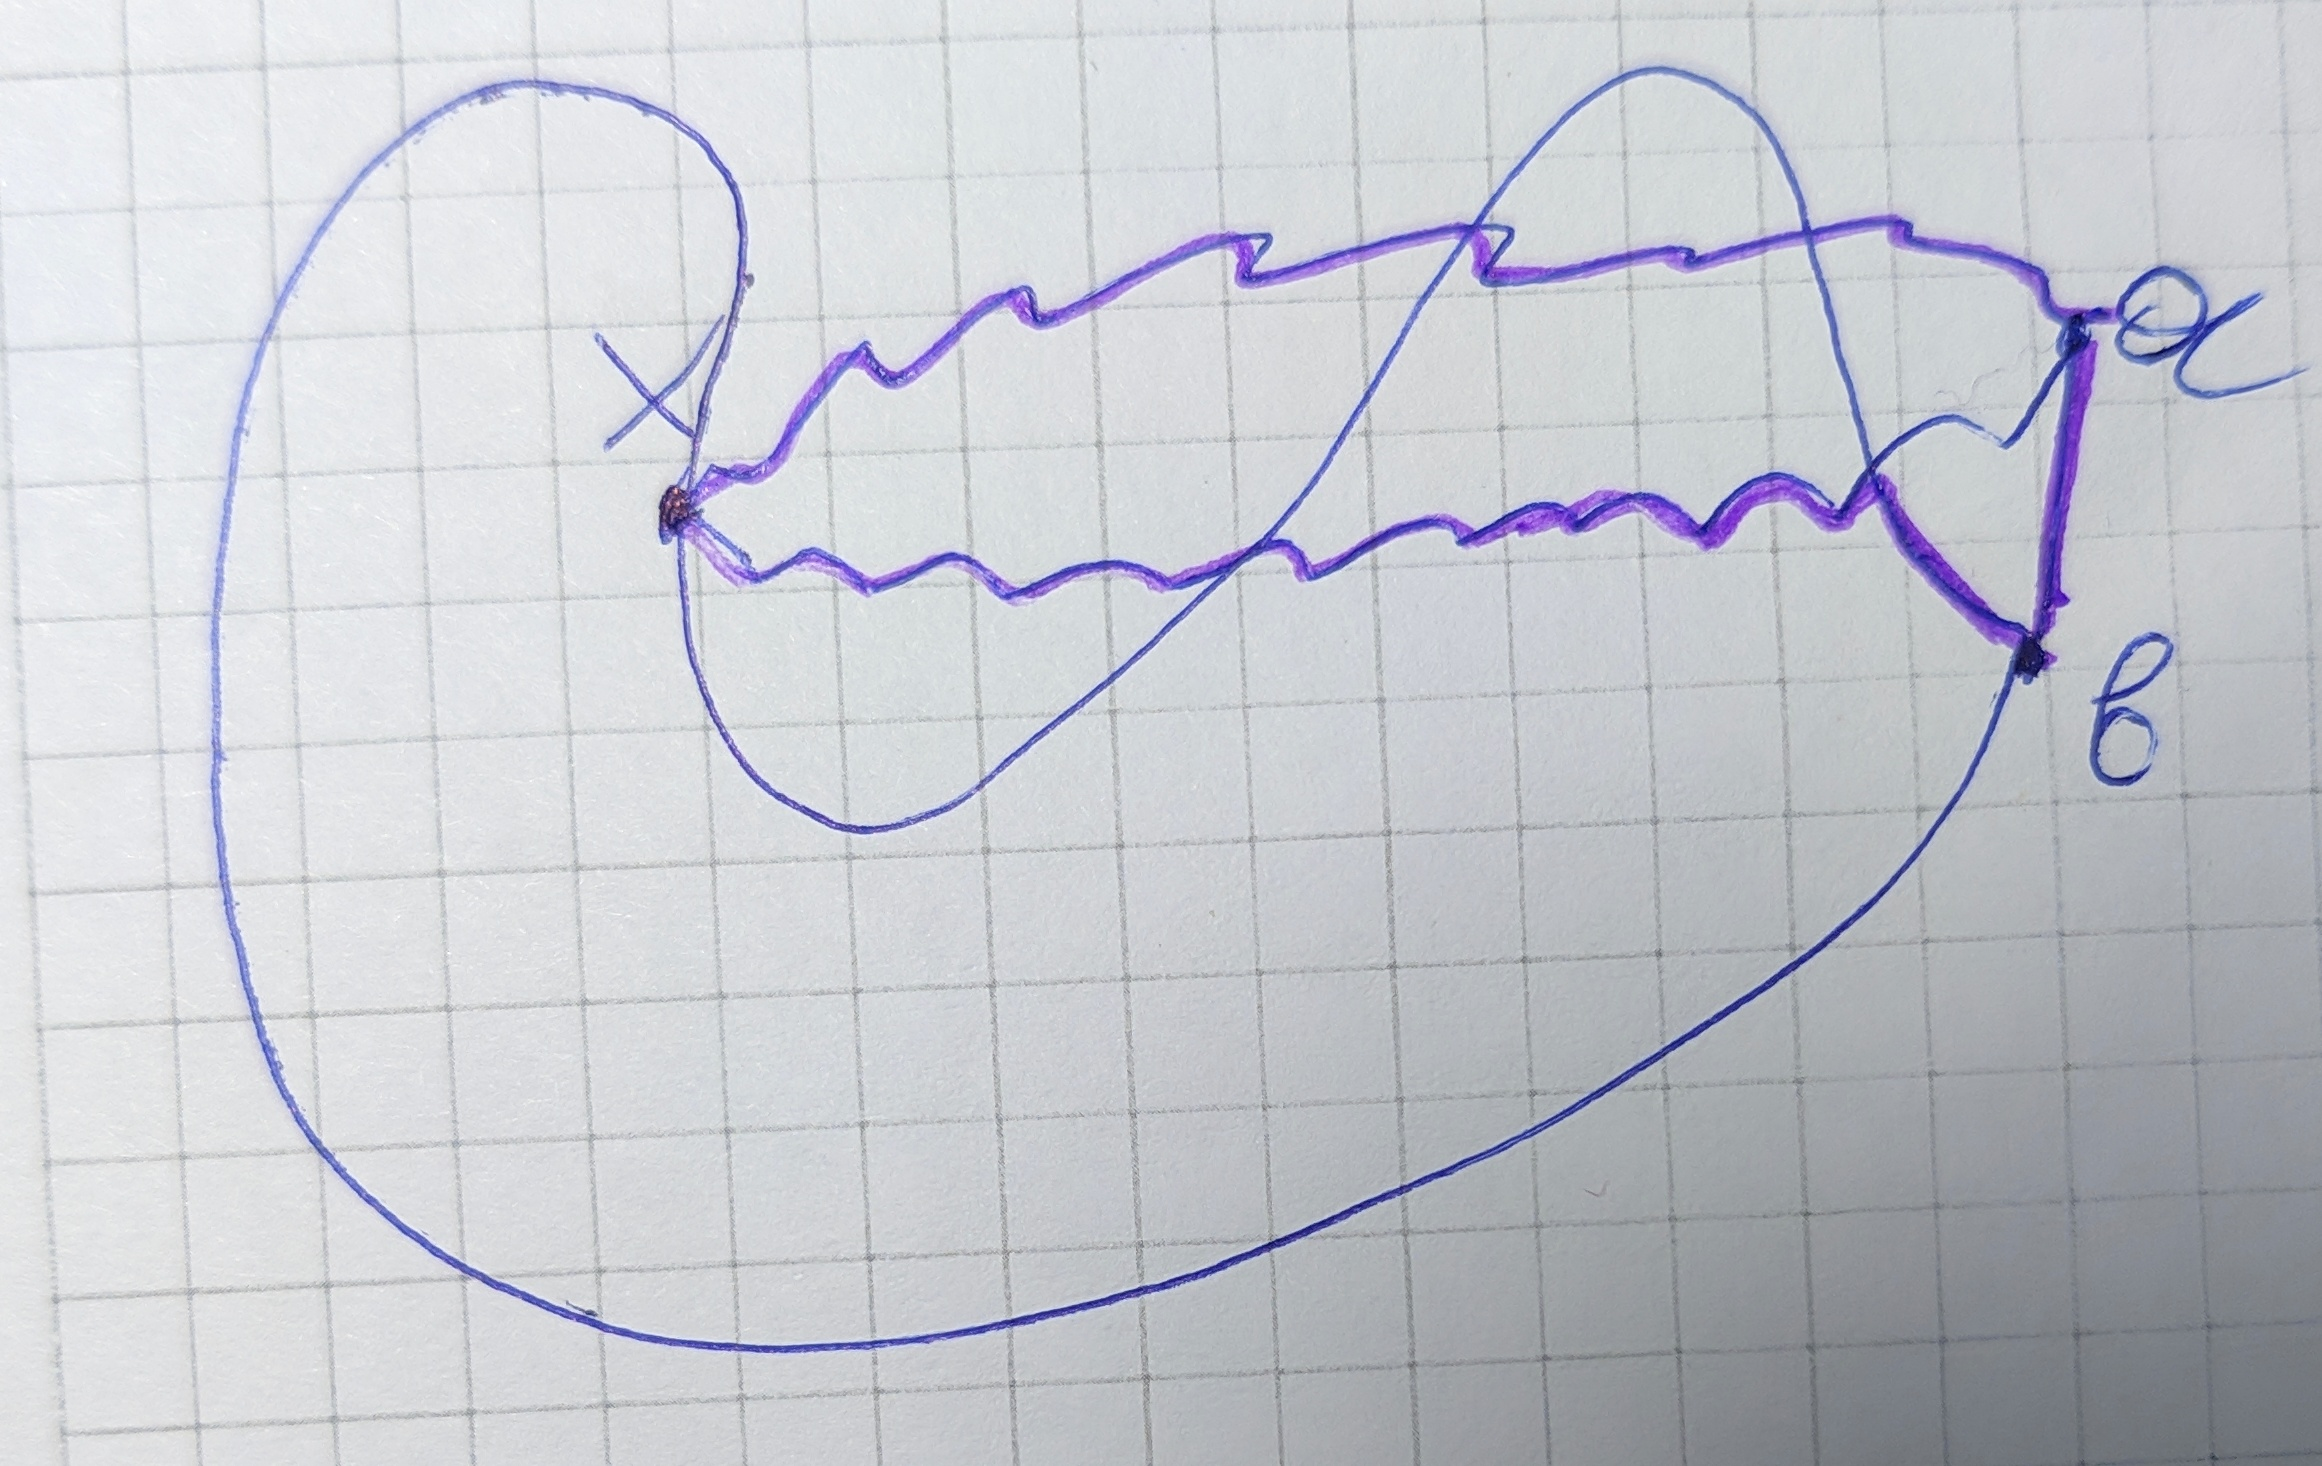
\includegraphics[width=250pt]{1}\\
		\\
		Остальное в качестве упражнения.\\
	\qedsymbol

\section{Теорема Менгера}
		Минимальное число вершин, разделяющих две несмежные вершины $u$ и $v$ равно максимальному числу попарно непересекающихся простых $(u,v)$-цепей.
	\begin{proof}
		(не вникал в доказательство, но идейно оно такое же как и на лекциях)\\
		Наибольшее число попарно непересекающихся простых $(u,v)$-цепей не больше минимального числа вершин, разделяющих $u$ и $v$ (поскольку можем удалить по вершине в каждой из этих $(u,v)$-цепей и разделить т.о. вершины u и v).\\
		Докажем, что если наименьшее число вершин, разделяющих $u$ и $v$ в графе $G$ равно $k$, то существует $k$ попарно непересекающихся простых цепей.\\
		При $k=1$ — очевидно.\\
		Пусть для некоторого $k>1$ — неверно. Пусть $t$ — наименьшее такое $k$. $F$ — граф с наименьшим числом вершин, для которого не выполненено условие
		(которое после слова ``доказать'') для $t$.\\
		Будем удалять из $F$ рёбра до тех пор, пока не получим некоторый граф $G$ такой, что $\forall e \in EG$ для разделения $u$ и $v$ в графе $G$ надо $t$ вершин,
		а в графе $G-e$ надо $t-1$ вершину.\\
		Т.о. имеется $G$ и $t$ такие, что теорема верна для
		\begin{enumerate}
			\item $\forall k < t$.
			\item $\forall$ графа с числом вершин, меньшим, чем $|VG|$.
			\item $\forall$ графа $G-e \, \forall e \in EG$.
		\end{enumerate}
		\textit{(док-во ниже)}
	\end{proof}

\subsection{Утверждение 1}
	В гарфе $G$ нет вершин, которые одновременно смежны с $u$ и $v$.
	\begin{proof}
		Пусть $w$ смежно с $u$ и $v$. Тогда в $G-w$ для разделения $u$ и $v$ достаточно $t-1$ вершины по пункту 2 в $G-w$ существует $t-1$ попарно непересекающихся
		простых $(u,v)$-цепей. Добавляем цепь $u,w,v \Rightarrow t$ попарно непересекающихся простых $(u,v)$ цепей в графе $G$. Противоречие с выбором графа $G$.
	\end{proof}
	
\subsection{Утверждение 2}
	Любое мно-во вершин $W$, разделяющих $u$ и $v$, $|W|=t$ смежно либо с $u$, либо с $v$.
	\begin{proof}
		Цепь, соединяющую $u$ с нек...
		
	\end{proof}

\begin{proof}\textit{(продолжение)}\\
	Рассмотрим некоторе $e=xy \in EG$. По условию 3 в $G-e$ существует $t-1$ вершина, разделяющая $u$ и $v$.\\
	В $(G-S_e)$ существует $(u,v)$-цепь и каждая точка цепи содержит ребро $e$.\\
	$(**)\forall e = xy: \Rightarrow $ 1) $x,y \not\in S_e$\\
	2) если $x\ne u, x \ne v$, то $S_e \cup \{x\}$ разделяет $u$ и $v$ в $G$.\\
	Рассмотрим кратчайшую $(u,v)$-цепь в графе $G$. $P=u, x_1, x_2, x_3, ..., x_m, v$.\\
	Рассмотрим $e=x_1x_2$. Из утвержджения 1 $x_2 \ne v$.\\
	$S_e = \{ y_1, ..., y_{t-1} \}$\\
	$W_1 = S_e \cup \{x_1\}$ по (**) разделяет $u$ и $v$. По утверждению 1, $x_1,v \not\in EG$. По утверждению 2, $W_1$ смежно с $u$. $\{y_1, ..., y{t-1} \}$ смежно с $u$ и не смежно с $v$.\\
	$W_2 = S_e \cup \{x_2\}$ по (**) разделяет $u$ и $v$. По утверждению 2 $x_2$ смежно с $u$. Противорчеие с выбором кратчайшей цепи
\end{proof}	

\section{Независимое множество. Оценки числа независимости. Вершинное покрытие. Связь чисел покрытия и независимости.}
\subsection{Независимое множество.}
	Мно-во вершин $W\subseteq VG$ называется \textbf{независимым}, если $\forall w, u \in W \quad uw\not\in EG$.\\
		Независимое мно-во \textbf{тупиковое (максимальное)}, если оно не является собственным подмножеством другого независимого мно-ва.\\
	Независимое мно-во наибольшей мощности - \textbf{наибольшее} назависимое мно-во. Мощность такого мно-ва называется \textbf{числом независимости} $\alpha_0(G)$
\subsection{Оценки числа независимости.}
	$ \displaystyle \forall G \quad \alpha_0(G) \ge \sum_{v \in VG} (1+ \operatorname{deg}(v))^{-1}$
	\begin{proof}
		Пусть $G = K_n$. Тогда $\alpha_0(K_n) = 1$.\\
		$ \displaystyle \sum_{v \in VG} n^{-1} = \frac{n}{n} = 1$.\\
		Индукция по числу вершин для $G\ne K_n$:\\
		$|VG| \le 2$ - всё очевидно.\\
		Пусть $|VG| = n \ge 3$, для любого графа с меньшим число вершин теорема верна, $ G \ne K_n$.\\
		Выбираем $x$ - вершинка $G$ наименьшей степени. Т.к. $ G \ne K_n$, то $x \cup N(x) \ne VG$.\\
		$G' = G - x - N(x)$. По индукционному предположению в $ \displaystyle G': \, \alpha_0(G') \ge \sum_{v \in VG'} (1+ \operatorname{deg}(v))^{-1}$.\\
		Пусть $M' \subseteq VG', \, M'$ - независимо в $G'$, $|M'| = \alpha_0(G')$.\\
		$v \cup M'$ - независимо в $G \quad  \Rightarrow  \quad \alpha_0(G) \ge |x \cup M'| = \alpha_0(G')+1$.\\
		$\forall v \in VG' \quad  \operatorname{deg}_G(v) \ge  \operatorname{deg}_{G'}(v)$\\
		$ \displaystyle \sum_{v \in VG'} (1+ \operatorname{deg}_{G'} v)^{-1} \ge\sum_{v \in VG'} (1+ \operatorname{deg}_{G} v)^{-1}$\\
		$\forall v \in N(x) \quad  \operatorname{deg}_G(v) \ge  \operatorname{deg}_G(x)$ (т.к. $x$ — вершина с наименьшей степенью в G)\\
		$ \displaystyle \sum_{v \in N(x)} (1+ \operatorname{deg}_G(v))^{-1} \le \sum_{v \in N(x)}( \operatorname{deg}_G(x)+1)^{-1} = \frac{ \operatorname{deg}_G(x)}{\operatorname{deg}_G(x)+1}$\\
		Берём неравенства 1 и 3 строчками выше и подставляем их куда-то в начало:\\
		$ \displaystyle \alpha_0(G) \ge 1 + \sum_{v \in VG'} (1+ \operatorname{deg}_G(v))^{-1} \ge \frac{ \operatorname{deg}_G(x)+1}{\operatorname{deg}_G(x)+1}+\sum_{v\in VG'}(1+ \operatorname{deg}_G(v))^{-1} = \frac{ \operatorname{deg}_G(x)}{1+\operatorname{deg}_G(x)} + (1+ \operatorname{deg}_G(x))^{-1} + \sum_{v \in VG'} (1+ \operatorname{deg}_G(v))^{-1}$
		$ \displaystyle \ge \sum_{v \in N(x)}( \operatorname{deg}_G(v)+1)^{-1} + (1+ \operatorname{deg}_G(x))^{-1} + \sum_{v \in VG'}(1 +  \operatorname{deg}_G(v))^{-1} = \sum_{v\in VG}(1+ \operatorname{deg}_G(v))^{-1}$
	\end{proof}
\subsection{Вершинное покрытие.}
	Вершина покрывет рёбра, инциндентные ей. Мно-во вершин, покрывающих все рёбра - \textbf{покрытие} (вершинное покрытие).\\
	Покрытие $W$ - тупиковое (минимальное), если $\forall V \subset W, \, V$ - не покрытие. Покрытие наименьшей мощности - наименьшее покрытие и его мощность
	Обозначается $\beta_0(G)$ - число покрытия графа $G$.
\subsection{Связь чисел покрытия и независимости.}
	Для $\forall$ G: $\alpha_0(G)+\beta_0(G)=|VG|$\\
\textbf{Доказательство:}\\
	Берём S — независимое: $|S| = \alpha_0(G)$\\
	По лемме 2.19 из лекций ($S \subseteq VG$ — независимое $\Leftrightarrow VG \setminus S$ — вершинное покрытие)\\
	$VG\setminus S$ — вершинное покрытие\\
	$\beta_0(G) \leqslant |VG \setminus S| = |VG| - \alpha_0(G)$ $\Rightarrow$ $\alpha_0(G) + \beta_0(G) \leqslant |VG|$\\\\
	Теперь, пусть $P$ — вершинное покрытие: $|P| = \beta_0(G)$\\
	По лемме 2.19 $VG \setminus P$ — независимое множество\\
	$\alpha_0(G) \geqslant |VG \setminus P| = |VG| - \beta_0(G)$ $\Rightarrow$ $\alpha_0(G) + \beta_0(G) \geqslant |VG|$\\
	$\Downarrow$\\
	$\alpha_0(G) + \beta_0(G) = |VG|$\\
	\qedsymbol

\section{Паросочетание, реберное покрытие. Теорема о связи чисел паросочетания и реберного покрытия. Совершенное паросочетание.}
	\subsection{Паросочетание, реберное покрытие.}
		$M \subseteq EG$ — паросочетание, если $\forall e,h \in M$ $e,h$ — не смежны.\\
		Наибольшее по мощности паросочетание — наибольшее паросочетание. Его мощность — число паросочетания $\alpha_1(G)$\\
		$Q \subseteq EG$ — рёберное покрытие, если оно покрывает все вершины\\
		Наименьшее по мощности рёберное покрытие — мин. рёберное покрытие. Его мощность — число рёберного покрытия $\beta_1(G)$
	\subsection{Теорема о связи чисел паросочетания и реберного покрытия.}
		$\forall$ G без изолированных вершин\\
		$\alpha_1(G) + \beta_1(G) = |VG|$\\
		\textbf{Доказательство:}\\
			Пусть $\alpha_1 = \alpha_1(G), \, \beta_1 = \beta_1(G), \, |VG|=n$\\
		Докажем: $\alpha_1 + \beta_1 \le n \quad \alpha_1 + \beta_1 \ge n$
		\begin{enumerate}
			\item Пусть $M$ - наибольшее паросочетание в $G$. Пусть $V'$ - мно-во вершин, не покрытых $M$. \\
				Либо $V'$ - пусто, либо $V'$ - независимое мно-во вершин (т.к. иначе M — не наибольшее паросочетание). Для каждой вершины из $V'$ выберем ребро, инциндентне ей. получаем $E'$. (если $V' = \varnothing  \Rightarrow E' = \varnothing$).\\
				Поскольку $V'$ - независимо, то $|E'| = |V'|$.\\
				По построению $V'$: $|V'| = n - 2 \cdot \alpha_1$\\
				$E' \cup M$ - рёберное покрытие $\beta_1 \le |E' \cup M| = |E'| + |M| = n - 2\alpha_1 + \alpha_1 = n - \alpha_1$.
			\item Пусть $P$ - наименьшее рёберное покрыти графа $G$. $G' = G[P]$. В $G'$ нет циклов (были бы, могли бы убрать одно ребро)\\
				Получаем, что $G'$ — ациклический граф, т.е. $G'$ — лес\\
				Каждая компонента связности графа $G'$ - дерево. Пусть $t$ компонент связности и число рёбер $k_1, k_2, ..., k_t$.\\
				В каждой компоненте выберем по одному ребру $ \Rightarrow $ получим паросочетания $M$. $|M| = t$.\\
				Имеем, $t \le \alpha_1$. Получаем, что $ \displaystyle n = \sum_{i=1}^t (k_i + 1) = t + \sum_{i=1}^t k_i = t + \beta_1 \le \alpha_1 + \beta_1$.
		\end{enumerate}
		\qedsymbol
	\subsection{Совершенное паросочетание.}
		Совершенное паросочитание — паросочитание, являющееся рёберным покрытием.
\section{Терема Кенига о числе паросочетания для двудольных графов. Теорема Кенига о (0,1)-матрицах.}
	\subsection{Терема Кенига о числе паросочетания для двудольных графов.}
			Для любого двудольного графа $G$: $\alpha_1(G) = \beta_0(G)$.
	\begin{proof}
		Пусть $G$ — граф. Докажем, что $\alpha_1(G) \ge \beta_0(G)$.\\
		Обозначин $\beta_0 = \beta_0(G)$\\
		Удаляем рёбра из $G$ пока не получим некоторый граф $G'$: $\beta_0(G') = \beta_0$ и $\forall e \in EG' \quad \beta_0(G'-e)=\beta_0-1$.\\
		
		Докажем утверждение, что в $G'$ нет смежных рёбер.\\
		Пусть это гон и в $\exists e,g \in EG'$: $e$ и $g$ смежны в $G'$, общая вершина $v$. В графе $G'-e$ существуют вершин. покрытие $S_e \quad |S_e|=\beta_0-1$ и
		концы ребра $e$ не лежат в $S_e$.\\
		В графе $G'-g$ существует вершинное покрытие $S_g$ и концы ребра $g$ не принадлежат $S_g$.\\
		Рассмотрим порождённый подграф графа $G'$: $G''=G'[\{v\} \cup (S_e \setminus S_g) \cup (S_g \setminus S_e)]$\\
		$|S_e \cap S_g| = t \quad |VG''|=1+\beta_0-1-t+\beta_0-1-t=1+2(\beta_0-1)-2t$\\
		$G''$ подграф графа $G \quad \Rightarrow  \quad G''$ - двудольный.\\
		Пусть $A$ - меньшая доля графа $G$.\\
		$|A| \le \frac{1}{2}|VG''| = \beta_0-1-t$. $A$ - вершинное покрытие $G''$.\\
		Покажем, что $A'=A \cup (S_e \cup S_g)$ - вершинное покрытие $G'$.\\
			Возьмём произвольное ребро. Пусть $h \in EG'$.\\
			\begin{enumerate}
				\item $h\in\{e, g\}$\\
					$e,g \in EG'' \Rightarrow e,g$ покрыты мно-ом $A$, а значит и $A'$.	
				\item $h\not\in\{e, g\}$\\
					Тогда $h$ покрывается как $S_e$, так и $S_g$.
					\begin{enumerate}
						\item $x \in S_g \quad x \in S_e \Rightarrow x \in S_g \cap S_e \Rightarrow$ покр. $A'$.
						\item один конец приндалежит $S_e \setminus S_g$, а другой: $S_g \setminus S_e \Rightarrow h \in EG'' \Rightarrow h$ покрывается $A$.
					\end{enumerate}
			\end{enumerate}
			Следовательно $\beta_0(G') \le |A'| \le |A| + |S_e \cap S_g| \le \beta_0-1-t + t = \beta_0-1$ - противоречие с выбором графа $G'$ (противоречие с тем, что
			существуют 2 смежных ребра).\\
			
	Граф $G'$ состоит из независимых рёбер. $\beta_0(G') = \alpha_1(G') \quad \beta_0(G) = \beta_0(G') = \alpha_1(G') \le \alpha_1(G)$.\\
	Из леммы 2.23($\forall G \quad \alpha_1(G) \leqslant \beta_0(G)$, это верно т.к. чтобы покрыть все рёбра, надо покрыть и все рёбра паросочетания) следует, что $\beta_0(G) = \alpha_1(G)$.
	\end{proof}
	\subsection{Теорема Кенига о (0,1)-матрицах.}
			Для любой (0, 1)-матриц максимальное число единиц, никакие 2 из которых не стоят в одном столбце и в одной строке, равно минимальному числу строк и столбцов,
	содержащих все единицы.
	\begin{proof}
		Пусть $G$ - двудольный граф, с долями $\{ v_1, v_2 ... v_n\}, \, \{ u_1 ... u_n \}$. Матрица смежности двудольного графа $G$:\\
		$A(G) = (a_{ij}) \mid a_{ij} = \begin{cases} 1,  \quad v_iu_j \in EG \\ 0, \quad else \end{cases}$. \quad
\begin{tabular}{|l|l|}
\hline
0 & $A$\\
\hline
$A^T$ & 0 \\
\hline		                                                                                                          \end{tabular}\\
		Биекция между двудольным графом с долями мощности $n$ и $m$ и множеством (0,1)-матриц размера $n\times m$.\\
		Максимальное число единиц, никакие две из которых не стоят в одной строке или столбце равно $\alpha_1(G)$ для соотв. графа $G$.\\
		Минимальное число строк и столбцов, содержащих единицы равно $\beta_0(G)$ для соотв. графа $G$.
	\end{proof}

\section{Терема Холла о паросочетаниях.}
	Пусть $G = (A, B, E)$ - двудольный граф.\\
	В $G$ существует паросочетание, покр. $A \quad \Leftrightarrow \quad \forall X \subseteq A \quad |N(X)| \ge |X|$
	\begin{proof}\hfil
		\begin{description}
			\item[$ \Rightarrow $)] Если существет $X \subseteq A:  \quad |N(X)| < |X|$, тогда паросоч., покр. $X$ не существует: не хватит рёбер. А значит нет паросч., покрывающего $A$.
			\item[$ \Leftarrow $)]Док-во индукцией по числу вершин в доле $A$:\\
				Если $|A|=1$ - очевидно верно\\
				Пусть $|A| \ge 2$. Рассмотрим 2 случая:
				\begin{enumerate}
					\item $\forall X \subset A \quad |X| < |N(X)|$\\
						Выберем ребро $uv \in E \quad v\in A, u \in B$.\\
						Рассмотрим новый граф $G' = G- v-u$. Обозначим $A' = A \setminus \{ v\}$.\\
						Пусть $X \subseteq A'$. $|X| < |N_G(X)|$, $|N_{G'}(X)| \ge |N_G(X)|-1$ ($-1$ на случай, если $y$ входит в $N(X)$)\\
						$|X| < |N_{G'}(X)|+1 \Rightarrow |X| \le |N_{G'}(X)|$.\\
						По индукционному предположению в графу $G'$ существуют паросчитания,
						покрывающие $A' \quad  \Rightarrow  \quad $ объединим его с ребром $vu \quad  \Rightarrow  \quad $ получаем паросчитание в $G$ покр. $A$.
					\item $\exists A' \subset A \quad |A'| = |N(A')|$\\
						Рассмотрим 2 порождённых подграфа:\\
						$G_1 = G[A' \cup N(A')]\\
						G_2 = G - A' - N_G(A')$\\
						Покажем, что $G_1$ и $G_2$ удовлетворяют условиям теоремы.\\
						В $G_1$: $\forall X \subseteq A' \quad N_G(X)=N_{G'}(X)$\\
						$|X| \le |N_G(X)| = |N_{G'}(X)| \quad  \Rightarrow  \quad G_1$ удовлетворяет условию теоремы.\\\\
						Пусть $X\subseteq A \setminus A'$. Рассмотрим $X \cup A'$ в $G$.\\
						$|X \cup A'| \le |N_G(X \cup A')| \le |N_{G_2}(X)| + |N_G(A')|$\\
						Вспоминаем, что $|A' \cup X| = |X| + |A'|$\\
						$|A'| = |N_G(A')|  \quad  \Rightarrow  \quad |X| \le |N_{G_2}(X)|$\\
						По индукционному предположению в $G_1$ существует паросоч., покрывающ. $A'$, в $G_2$ существует паросоч., покрывающ. $A\setminus A'$.
						Следовательно, их объединение - искомое паросоч., покр. $A$.
				\end{enumerate}
		\end{description}
	\end{proof}
\section{Теорема Фробениуса о свадьбах. Системы различных представителей, теорема Холла о СРП.}
	\subsection{Теорема Фробениуса о свадьбах.}
			Двудольный граф $G=(A,B,E)$ имеет совершенное паросочетание $ \quad \Leftrightarrow \quad |A|=|B|$ и для любого $X \subseteq A \quad |N_G(X)| \ge |X|$.\\
		\textbf{Доказательство:}\\
			В $G$ $\exists$ совершенное паросочетание $\Leftrightarrow$ $|A| = |B|$ и $\exists$ паросочетание покр. $A$ $\underset{\text{по т. Холла}}{\Leftrightarrow}$ \\$|A| = |B|$ и $\forall X \subseteq A \quad |N(X)| \leqslant |X|$\\
		\qedsymbol
	\subsection{Системы различных представителей}
		$A = \{a_1,\dotsc,a_m\}$ — некоторое множество\\
		$S = \{S_1,\dotsc,S_n\}$; $S_i \subseteq A \quad \forall i$; — семейство подмножеств множества $A$\\
		$x = (x_1,\dotsc,x_n)$ — система различных представителей для $S$ если:\\
		1) $x_i \in S_i \quad \forall i$;\\
		2) $x_i \neq x_j; \quad i \neq j$
	\subsection{теорема Холла о СРП.}
		$S = (S_1,\dotsc,S_n)$ имеет СРП $\Leftrightarrow$ $\forall k; \quad 1 \leqslant k \leqslant n \quad \forall \{i_1,\dotsc,i_k\} \subseteq\{1,\dotsc,n\} \quad |S_{i_1} \cup \dotsb \cup S_{i_k}| \leqslant k$\\
		\textbf{Доказательство:}\\
			$\Rightarrow$) Если посмотреть на определение, станет очевидно.\\
			$\Leftarrow$) Рассмотрим граф $G = (A, B, E)$\\
			$A = \{S_1,\dotsc,S_n\}$\\
			$B = \{a_1,\dotsc,a_m\}$\\
			$E = \{a_iS_j | a_i \in S_j\}$\\
			Когда $\exists$ паросочетание покрывающее A?\\
			(по т. Холлла) когда $\forall X \subseteq A \quad |N_G(X)| \leqslant |X| = k$\\
			$|N_G(X)| = |S_{i_1} \cup \dotsb \cup S_{i_k}|$\\
			Это условие выполняется $\Rightarrow$ $\exists$ паросочетание покр. $A$ $\Rightarrow$ существующее паросочетание определяет СРП\\
		\qedsymbol
\section{Теорема об увеличивающей цепи. Алгоритм построения наибольшего паросочетания в двудольном графе.}
	\subsection{Определения}
			$G$ — граф; $M$ — паросочетание\\
			цепь $x_1,\dotsc,x_t$ — $M$-чередующаяся $\Leftrightarrow$ $x_ix_{i+1} \in M$ $\Leftrightarrow$ $x_{i+1}x_{i+2} \notin M \quad \forall i$\\\\
			$M$-чередующаяся цепь $x_0,\dotsc,x_t$ — $M$-увеличивающаяся, если $x_0$ и $x_t$ не покрыты рёбрами из $M$
	\subsection{Теорема об увеличивающей цепи.}
		$M$ — паросочетание в G\\
		$M$ — наибольшее $\Leftrightarrow$ в $G$ нет $M$-увеличивающей цепи\\
	\textbf{Доказательство:}\\
		$\Rightarrow$) Пусть в $G$ существует $M$-увелич. цепь P. Тогда рассмотрим $M' = (M \setminus EP) \cup (EP \setminus M)$ – паросочетание (очевидно)\\
		$|M'| = |M| + 1$ – противоречие с тем, что M наибольшее.\\
		$\Leftarrow$) Рассмотрим $M'$ – пусть это наибольшее паросочетание в G.\\
		$G' = G[(M \setminus M') \cup (M' \setminus M )]$\\
		$\forall v \in G' \quad deg_{G'}(v) \leqslant 2 \Rightarrow$ каждая компонента связности графа G' – цикл или цепь.\\
		Если в какой-то компоненте связности $\exists$ цепь, в которой рёбер 1-го паросочетания больше рёбер другого $\Rightarrow$ $\exists$ либо $M$-увеличивающая цепь (противореч. с нач. усл.), либо $\exists$ $M'$-увеличивающая цепь (противореч. с $M'$—наиб.)\\
		$\Rightarrow$ $|M| = |M'|$ $\Rightarrow$ $M$ — наибольшее паросочетание\\
		\qedsymbol
	\subsection{Алгоритм построения наибольшего паросочетания в двудольном графе.}
		$G = (A,B,E)$
		\begin{enumerate}
			\item M — паросочетание
			\item $A_1 \subseteq A$, $B_1 \subseteq B$ — множества непокрытых M вершин; Организуем максимальный лес F в G:
			\begin{enumerate}
				\item $\forall b \in (VF \cap B) \quad deg_F(b) = 2$ и одно из этих $2$-х рёбер из M
				\item $\forall$ компонента связности леса $F$ содержит ровно 1-ну вершину из $A_1$. Добавим все оставшиеся вершины из $A_1$ в качестве одновершинных компонент связности графа $F$
			\end{enumerate}
			\item Если $\exists$ ребро между вершинами из $B_1$ и $VF$, то есть $M$—увеличивающая цепь начинающаяся с этого ребра. по пункту 32.2 строим новое паросочетание большей мощности и переходим на шаг 2)
			\item Если нет ребра, то $M$ — наибольшее паросочетание
		\end{enumerate}
\section{Эйлеров цикл, эйлеров граф. Теорема Эйлера. Алгоритм Флёри.}
	\subsection{Эйлеров цикл, эйлеров граф.}
		Цикл, содержащий все рёбра графа — эйлеров.\\
		Граф, в котором есть эйлеров цикл — эйлеров
	\subsection{Теорема Эйлера.}
		Для связного графа порядка $n \leqslant 2$ следующие условия эквивалентны:
		\begin{enumerate}
			\item G — эйлеров
			\item $\forall v \in VG \quad deg$ $v$ — чётна
			\item Множество рёбер можно разбить на циклы.
		\end{enumerate}
		\textbf{Доказательство:}\\
			1 $\Rightarrow$ 2) Эйлеров цикл проходит через $\forall$ вершину $v$ $k$ раз и содержит все рёбра $\Rightarrow$ $deg_G(v) = 2k$\\
			2 $\Rightarrow$ 3) все вершины чётные $\Rightarrow$ нет висячих вершин $\Rightarrow$ G – не дерево $\Rightarrow$ в нём есть циклы\\
			Пусть $G_1$ – максимальный подграф графа $G$, удовлетворяющий условию 3. Очевидно, что все вершины в нём имеют чётную степень.\\
			$G_2 = G-EG_1$\\
			в $G_2$ все вершины имеют чётную степень (т.к. чёт$-$чёт$=$чёт).\\
			Если $G_2$ пуст, то всё доказали, иначе в нём есть рёбра.\\
			Очевидно, что он не дерево, а значит в нём есть цикл. Противоречие с максимальностью $G_1$.\\
			3 $\Rightarrow$ 1) Рассмотрим разбиение рёбер графа G на наименьшее число циклов: $c_1,\dotsc,c_s$.\\
			Покажем, что s = 1:\\
			Пусть не так ($s > 1$). $\Rightarrow$ $\exists i \neq j$ | $c_i$ и $c_j$ имеют общую вершину, но не имеют общих рёбер. Склеим их в один цикл. Противоречие с выбором наименьшего числа циклов $\Rightarrow$ $s = 1$. Это и есть Эйлеров цикл.\\
		\qedsymbol

\subsection{Алгоритм Флёри.}
	Нахождение эйлерова цикла\\
		0. выбираем произвольную вершину $\delta$ в графе $G$; $G' = G$\\
		1. Выбираем ребро $e$ в графе $G'$ инцидентное $\delta$ и не мост (если это возможно).\\
		$G' = G' - e$ и переходим во второй конец $e$
\section{Гамильтонов цикл, гамильтонов граф. Теорема Оре. Теорема Дирака.}
\subsection{Гамильтонов цикл, гамильтонов граф.}
	Простой цикл, содержащий все врешины графа, называется \textbf{Гамильтоновым циклом}.\\
	Граф, содержащий Гамильтонов цикл, называется \textbf{Гамильтоновым}.\\
\subsection{Теорема Оре.}
	Если для любых двух несмежных вершин v, u верно $deg(v) + deg(u) \geqslant |VG|$, то G – гамильтонов.\\
	\textbf{Доказательство теоремы:}\\\\
		\textit{Утверждение:}\\
		Если в связном графе длина максимальной простой цепи равна $k$ и в нём существует простой цикл длины $k + 1$, то этот простой цикл является гамильтоновым.\\
	\textit{Доказательство утверждения:}\\
		Рассмотрим наш цикл $C_{k+1}$. Если C – не гамильтонов, G – связный $\Rightarrow$ $\exists$ $u$, $v$: $u \in C, v \notin C, uv \in EG$.\\ Пусть $e \in C$, $e$ инцидентноно $u$.\\
		$C - e + uv$ – простая цепь длины $k + 1$ – противоречие с максимальной длиной цепи.\\
		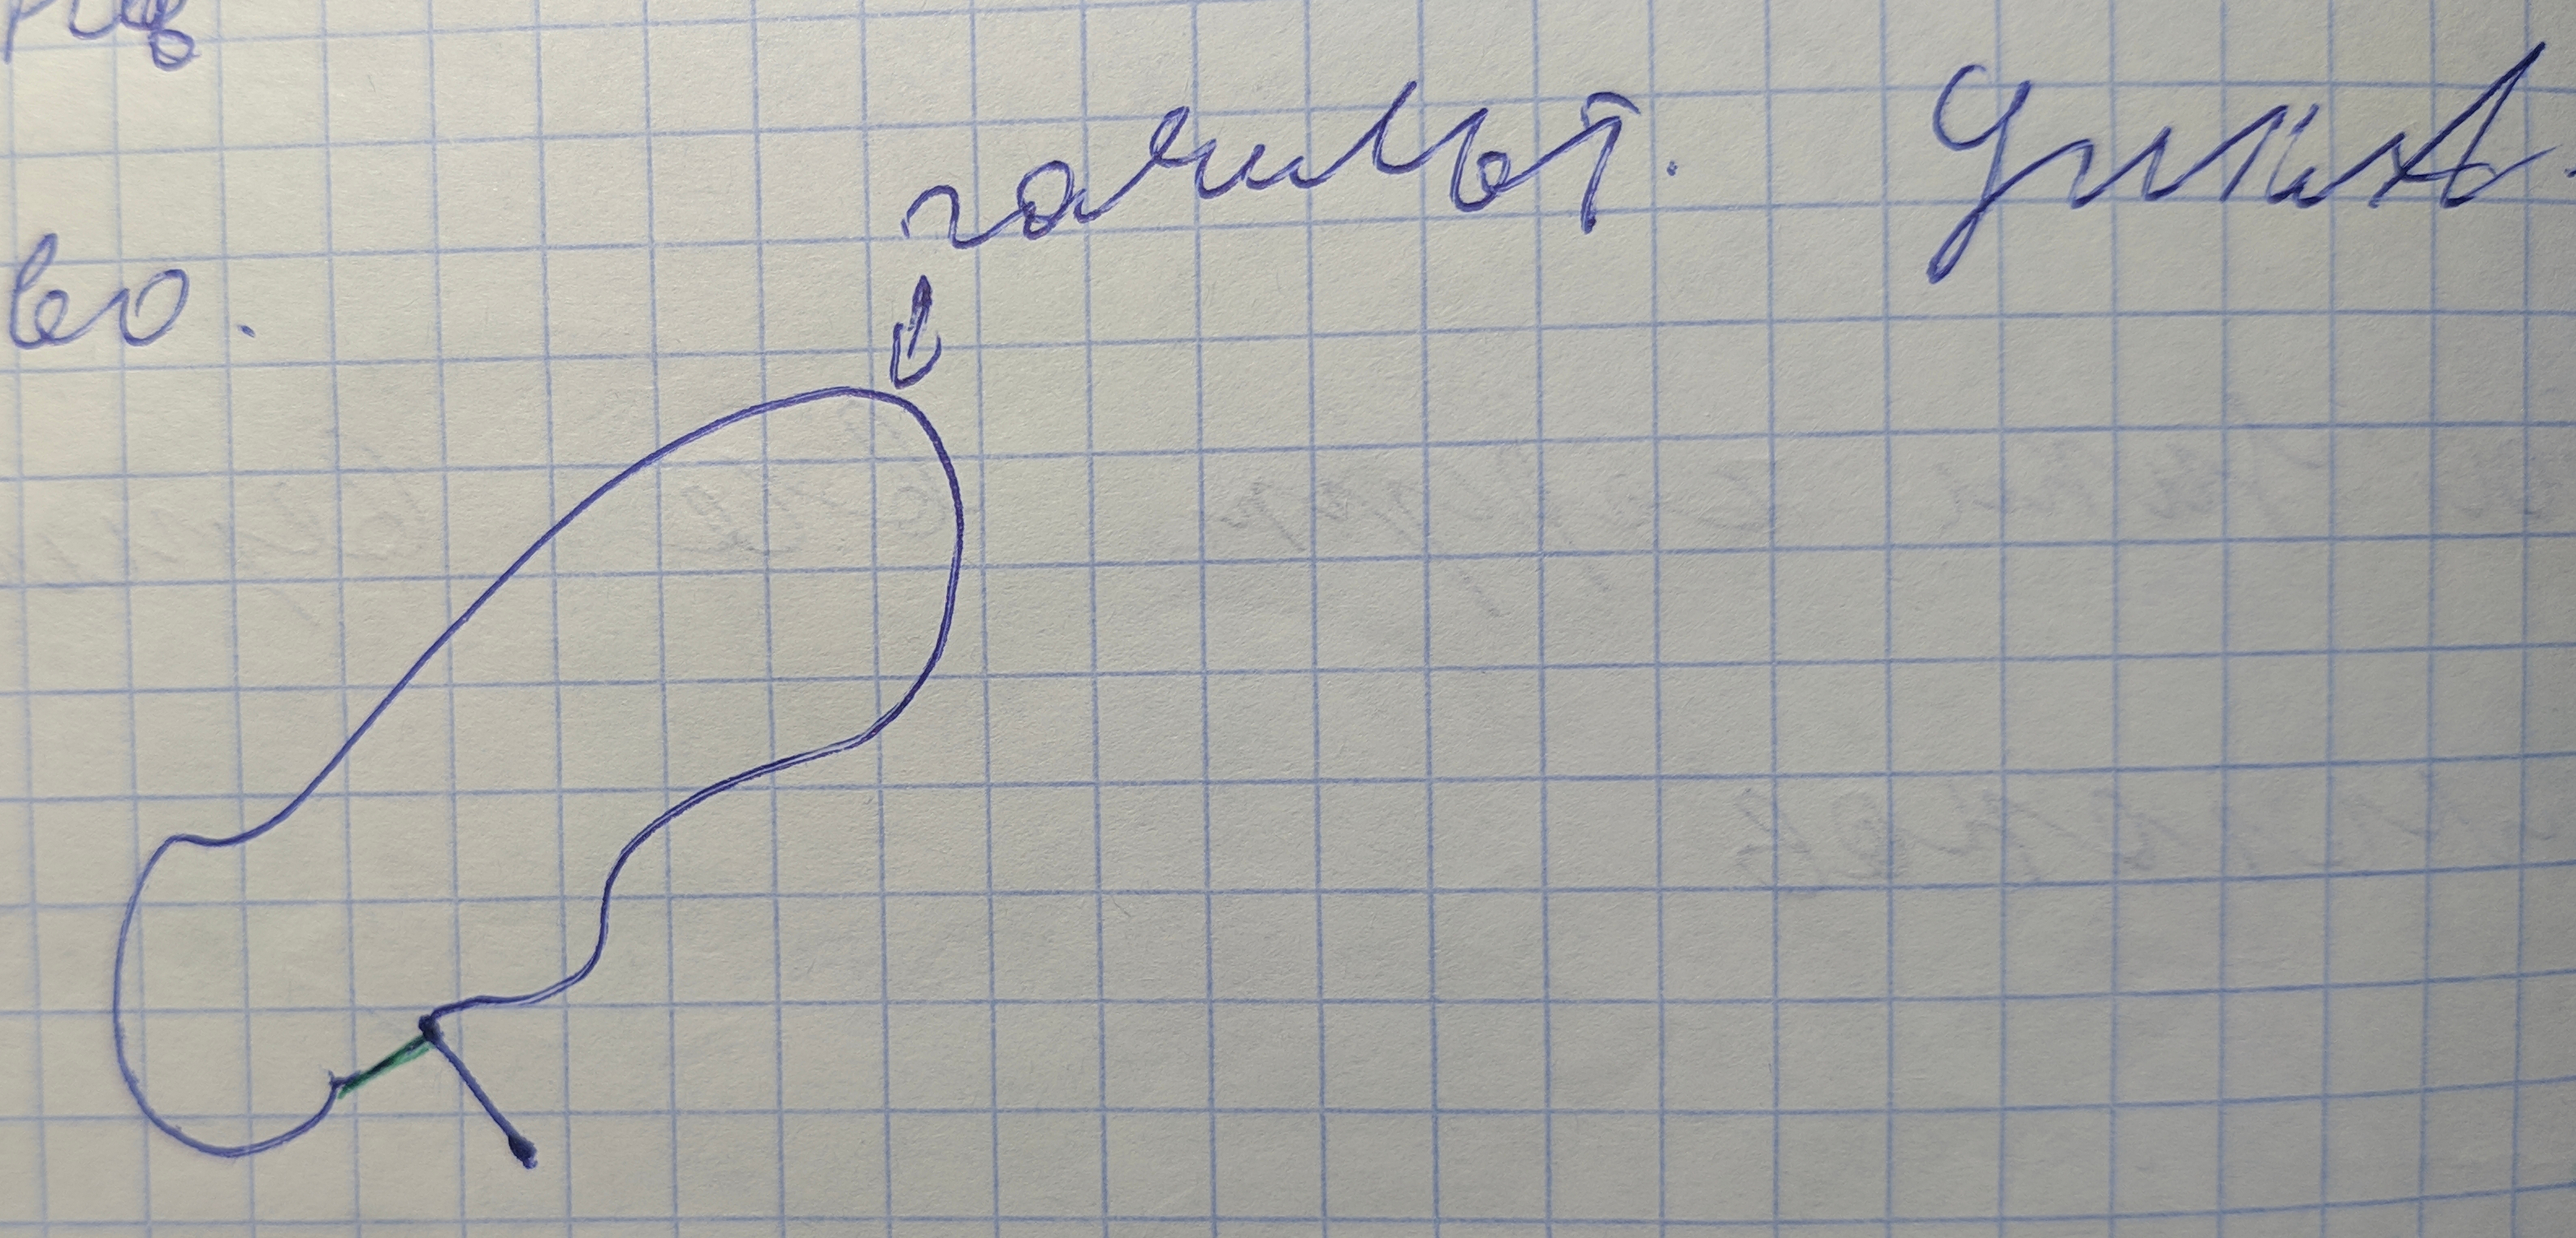
\includegraphics[width=250pt]{2}\\
	\qedsymbol\\\\
		Вернёмся к доказательству теоремы\\
		Рассмотрим самую длинну просутю цепь в графе $G$\\
		$v = x_0,\dotsc,x_t = u$\\
		Если $ub \in EG$, то получим цикл длины $t+1$ и он гамильтонов по утверждению\\
		Если $ub \notin EG$\\
		Знаем что $deg(u) + deg(v) \geqslant |VG|$\\
		Необходимо доказать что возможна ситуация как на изображениии:\\
		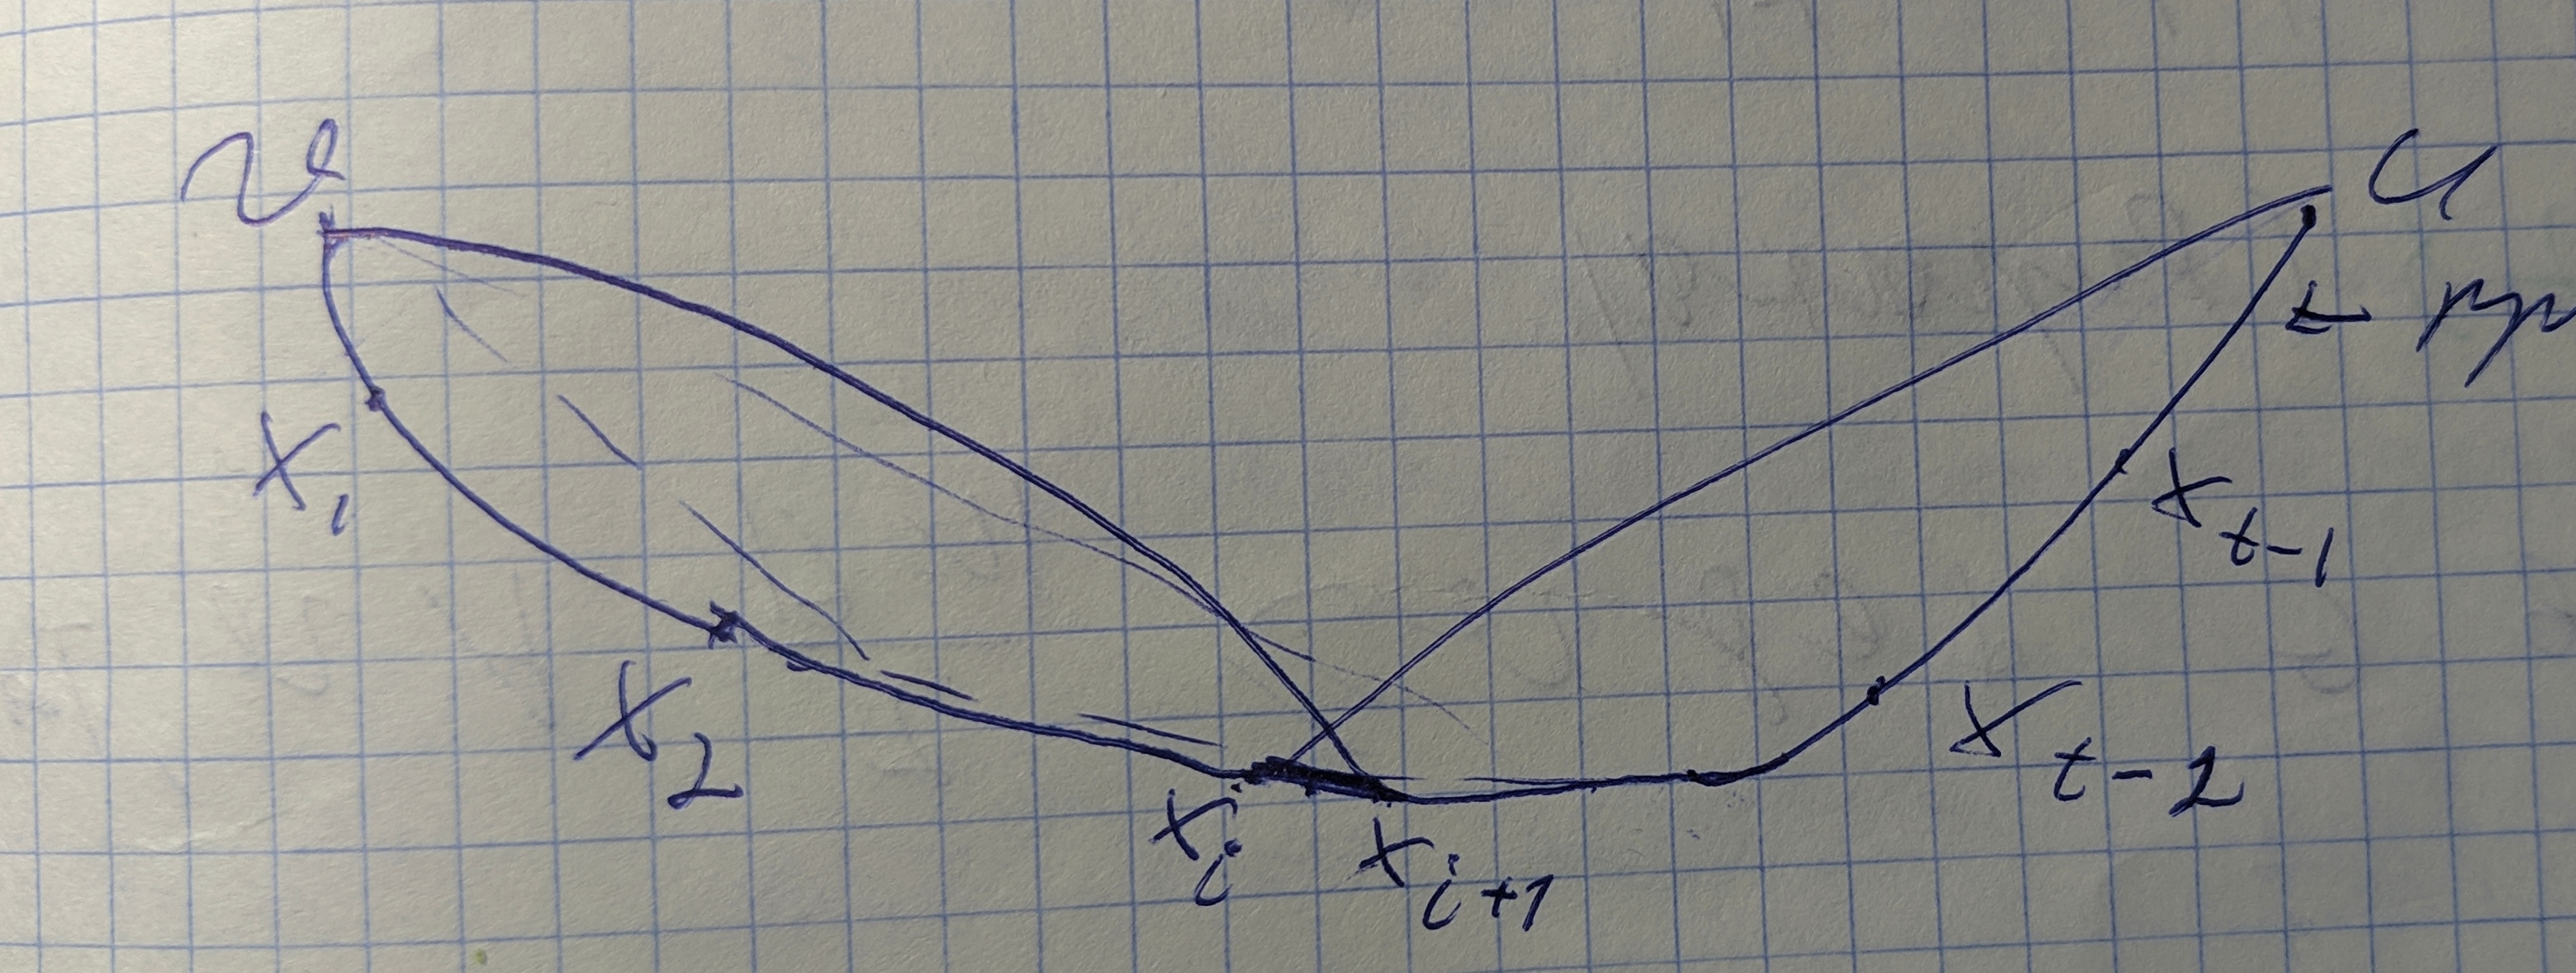
\includegraphics[width=250pt]{3}\\
		А именно: $\exists x_i,x_{i+1}$ т.ч. $x_i$ — смежна c $u$ и $x_{i+1}$ смежна с $v$\\
		Поскольку наша цепь длиннейшая, то все вершины, смежные с $v$ и смежные с $u$ лежат на этой цепи\\
		$I = \{i | x_iv \in EG, \quad 2 \leqslant i \leqslant t-1\}$\\
		$|I| = deg(v) - 1$\\
		$Y = \{j | x_{j-1}u \in EG, \quad 2 \leqslant j \leqslant t-1\}$\\
		$|Y| = deg(u) - 1$\\
		$|Y \cup I| \leqslant t-2$\\
		$|Y| + |I| = deg(v) + deg(u) - 2 \geqslant |VG| - 2 \geqslant t + 1 - 2 = t-1$\\
		т.е. $|Y \cup I| < |I| + |Y|$ $\Rightarrow$ $Y \cap I \neq \emptyset$ $\Rightarrow$\\
		$\exists i$: $vx_i,ux_{i-1} \in EG$\\
		Удаляем из цепи ребро между $x_{i-1}$ и $x_{i}$, добавляем рёбра $vx_i,ux_{i-1}$ и получаем цикл длины $t+1$\\
		Согласно утверждению, этот цикл являетя гамильтоновым.\\
		\qedsymbol

\section{Гамильтонов цикл, гамильтонов граф. Теорема Хватала-Эрдеша}
\subsection{Гамильтонов цикл, гамильтонов граф.}
	Простой цикл, содержащий все вершины графа — гамильтонов\\
	Граф, содержащий гамильтонов цикл — гамильтонов
\subsection{Теорема Хватала-Эрдеша}
	Пусть $G$ — связный граф порядка $n \geqslant 3$. Если $æ(G) \geqslant \alpha_0(G)$, то $G$ — гамильтонов\\
	\textbf{Доказательство:}\\
		Если $G$ нет циклов, то $G$ — дерево $\overset{n \geqslant 3}{\Rightarrow}$ $æ(G) = 1$; $\alpha_0(G) \geqslant 2$. Противоречие.
		$\Rightarrow$ в $G$  есть циклы\\
		Пусть C — самый длинный простой цикл\\
		Если $VC = VG$ — \qedsymbol\\
		Если $VG \setminus VC \neq \emptyset$\\
		Рассмотрим $G' = G - VC$\\
		Пусть $H$ — компонента связности $G'$\\
		$N_G(H) = \{x \in VG \setminus VH | \exists y \in H: xy \in EG\}$\\
		$N_G(H) \subseteq C$\\
		(*) Все вершины из $N_G(H)$ — попарно несмежные по циклу (иначе, есть простой цикл большей длины)\\
		$G - N_G(H)$ — несвязный граф (поскольку есть компонента H и остальное)\\
		$\Downarrow$\\
		$æ(G) \leqslant |N_H(H)|$\\
		S — множество правых соседей по циклу $C$ вершин из $N_G(H)$\\
		$|S| = |N_G(H)|$\\
		Покажем что $S$ — независимое множество в $G$\\
		Допустим что нет $\Rightarrow$ есть ребро между двумя вершинами из $S$ $\Rightarrow$ есть более длинный цикл (см. рисунок)\\
		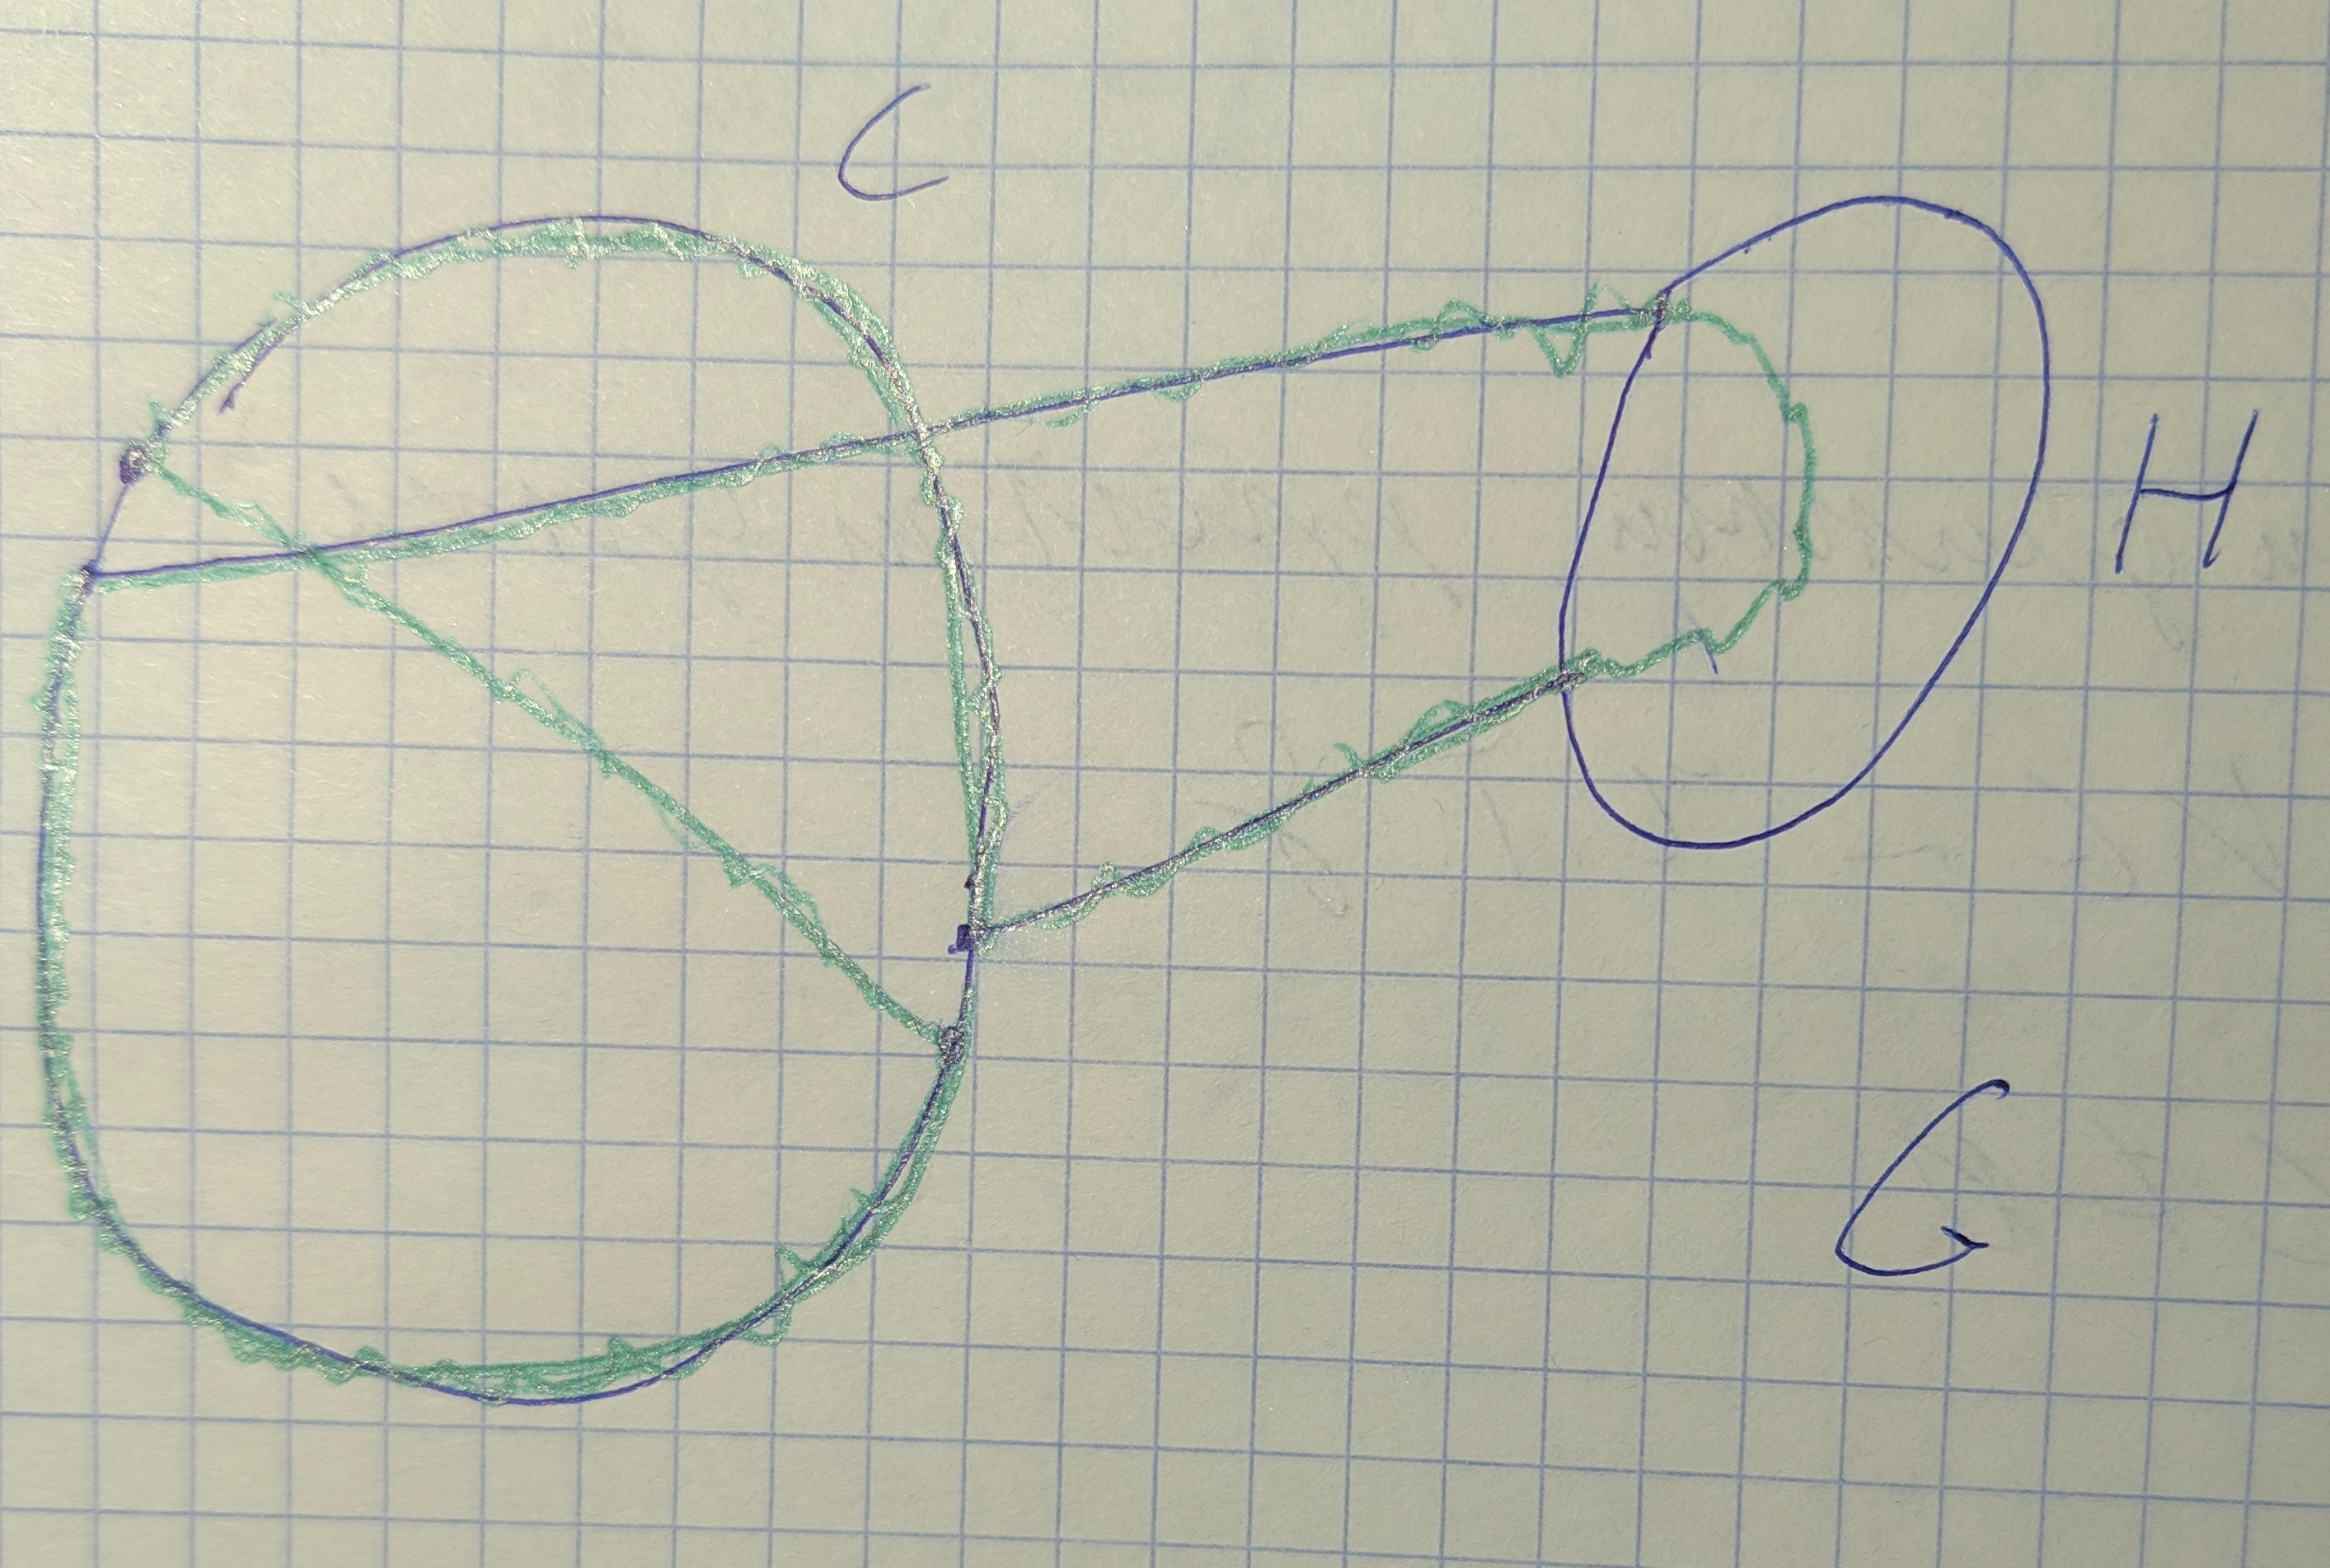
\includegraphics[width=250pt]{4}\\
		(*) $\Rightarrow$ $S \cap N_G(H) = \emptyset$ (иначе бы какая-то вершина из $N_G(H)$ являлась бы соседом др. вершине из $N_G(H)$ по циклу) $\Rightarrow$ $S \cup \{x\}$ — независимое множество $\Rightarrow$ $\alpha_0(G) \geqslant |S \cup \{x\}| = |N_G(H)| + 1 \geqslant æ(G) + 1$\\
		Противоречие с условием теоремы\\
		\qedsymbol

\section{Укладка графа в пространство. Планарный граф, плоский граф, укладка на сфере.}
	\subsection{Укладка графа в пространство.}
		Граф $G$ укладывается в про-во $\alpha$, если он изоморфен некоторому графу, вершинами которого являются точки этого пространства, а рёбра — кривые без самопересечений, соединяющие соответствующие вершины, при чём выполнены след. усл.:
		\begin{enumerate}
			\item кривая-ребро не содержит др. вршин графа кроме своих концов.
			\item 2 кривые-ребра пересекаются только в вершине инцидентной обоим рёбрам
		\end{enumerate}
	\subsection{Планарный граф, плоский граф, укладка на сфере.}
		Граф укладывающийся на плоскость — планарный\\
		Укладка планарного графа на плоскость — плоский граф\\\\
		Граф укладывается на плоскость $\Leftrightarrow$ он планарный\\
		\textbf{Доказательство:}\\
			Стереографическая проекция\\
			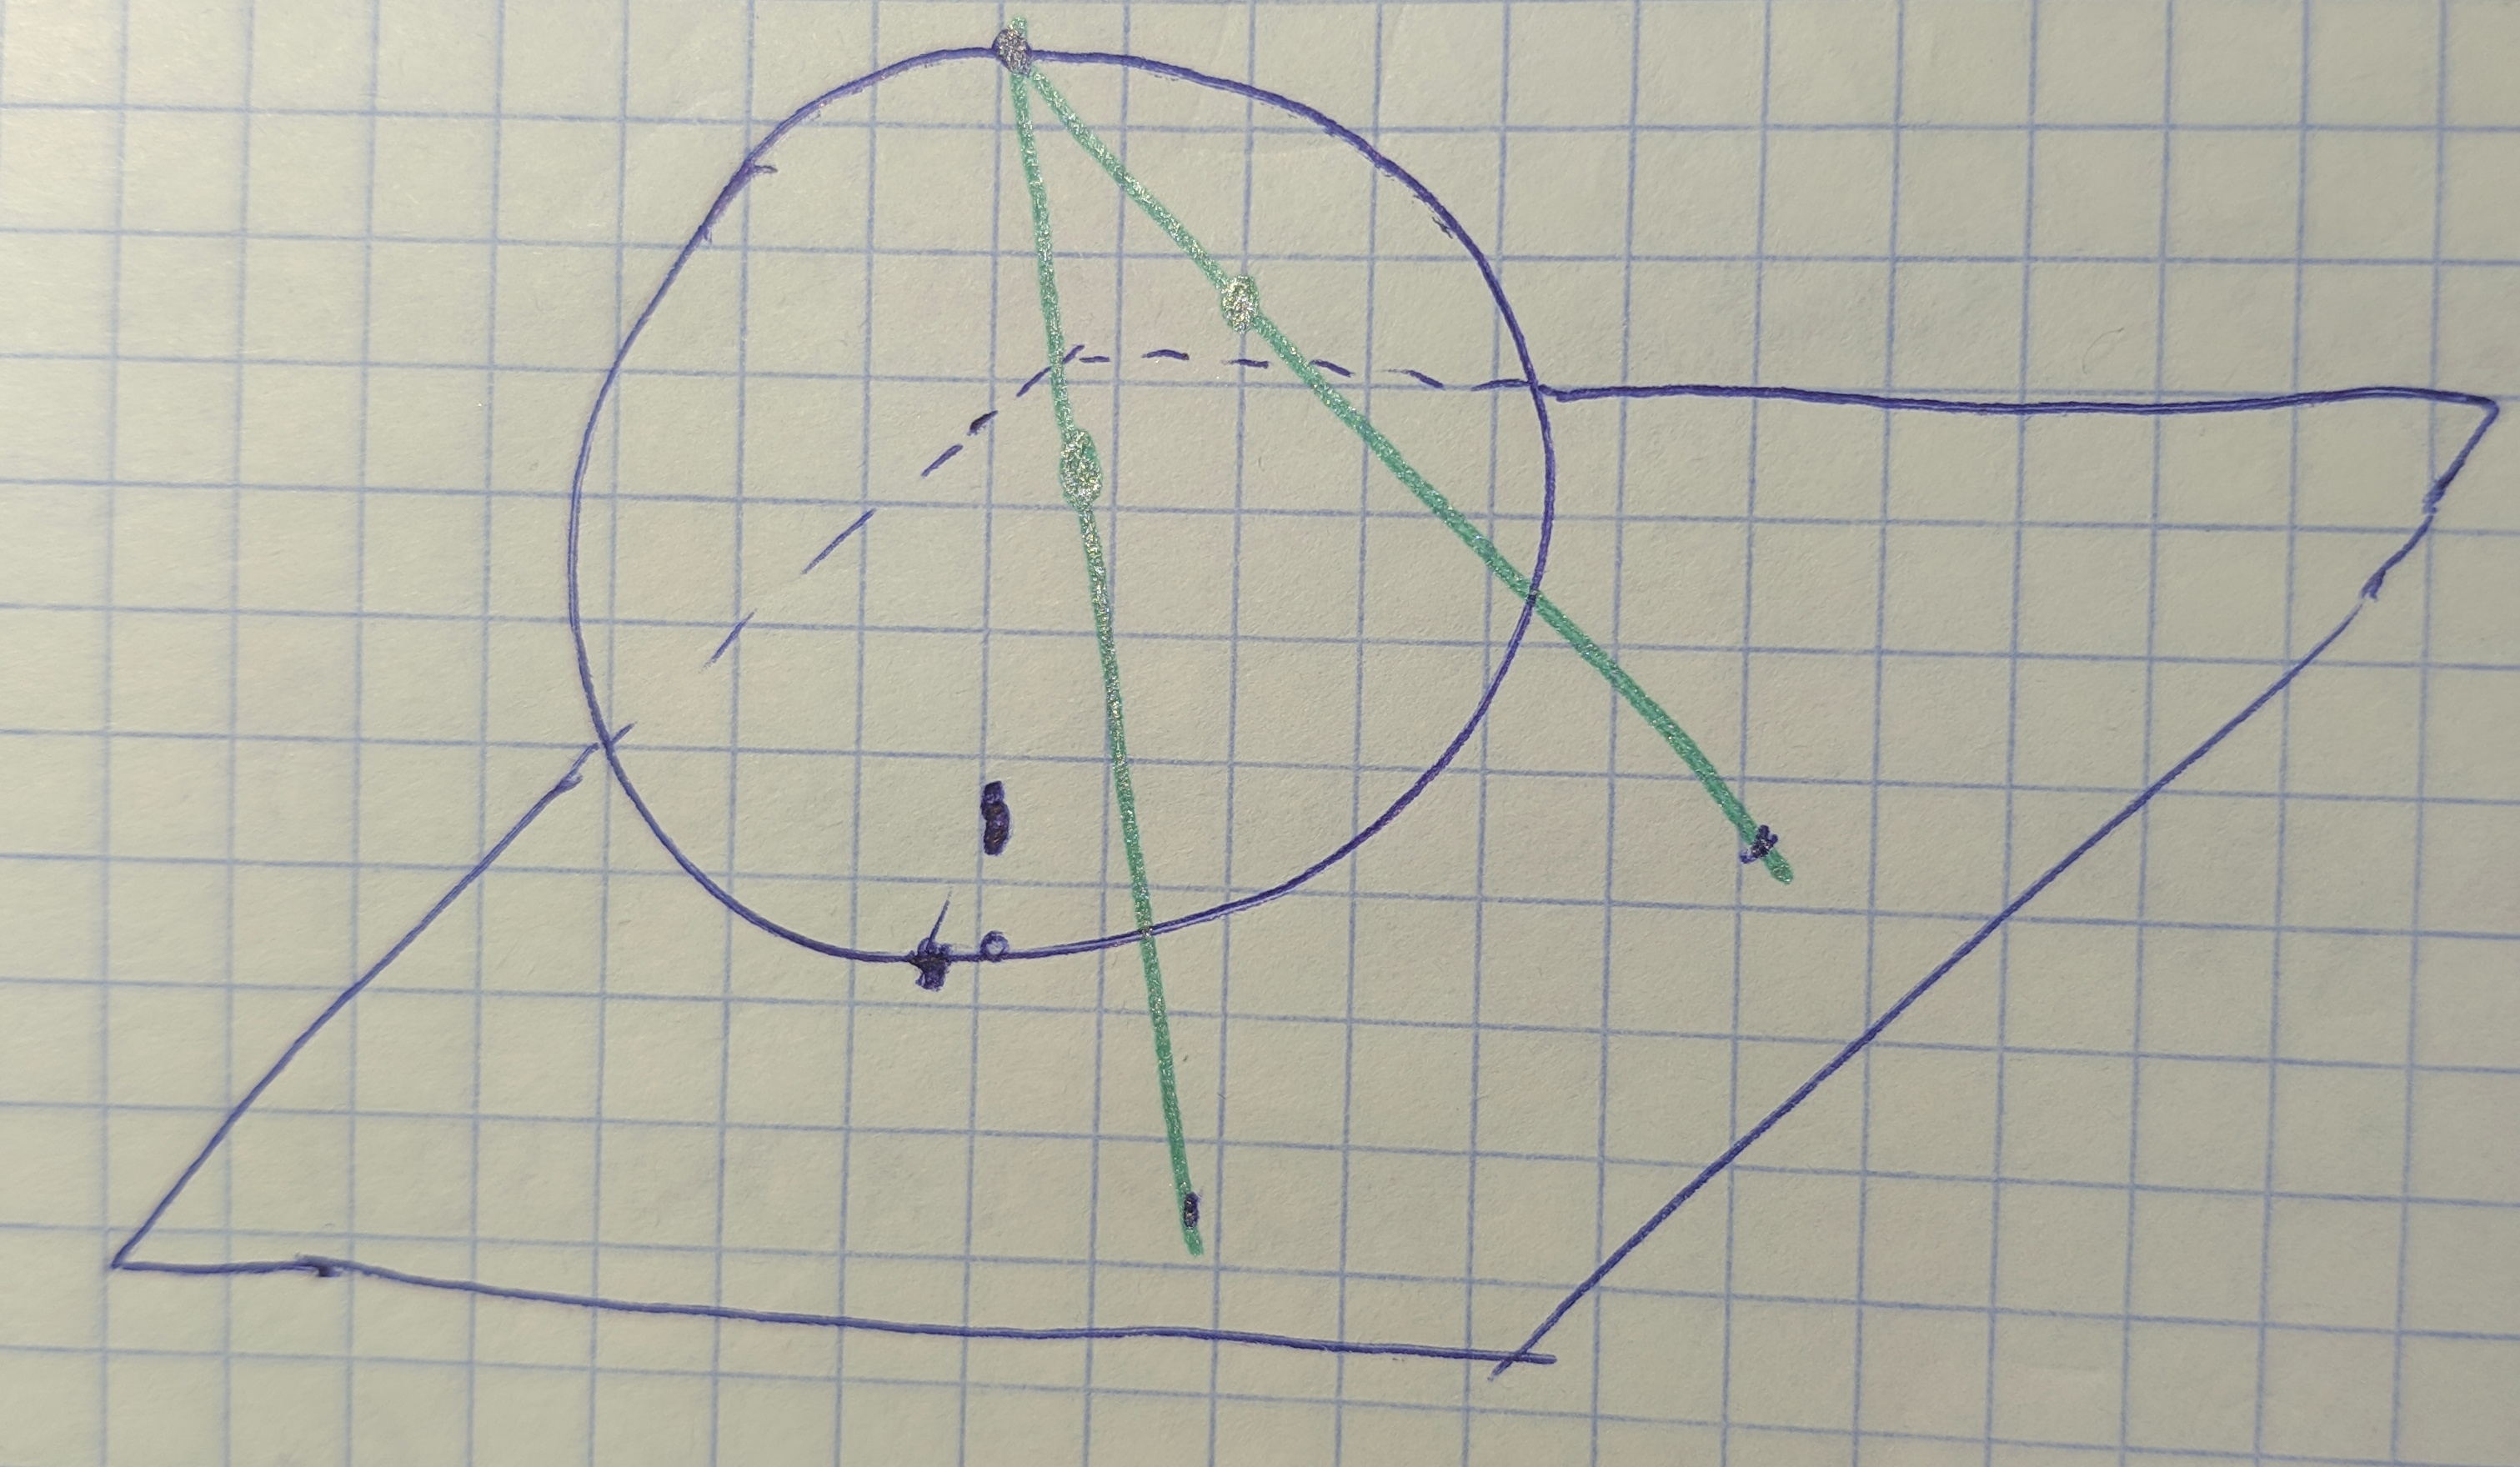
\includegraphics[width=250pt]{5}\\
		\qedsymbol

\section{Формула Эйлера. Непланарность $K_5$ и $K_{3,3}$. Критерии планарности.}
\subsection{Формула Эйлера.}
	$G$ — связный плоский граф $(n,m)$-граф с $f$ гранями, тогда $n - m + f = 2$\\
	\textbf{Доказательство:}\\
		Рассмотрим остовное дерево $T$ для $G$\\
		В $T$ n вершин, $n-1$ ребро, 1 грань\\
		$n - (n - 1) + 1 = 2$\\ т.е. ф-ла верна\\
		Добавление ребра грань на 2 грани\\
		+1 к грани и граням $\Rightarrow$ ф-лы остаётся верной\\
		т.о. мы можем приёти к графу $G$ и сохранить ф-лу\\
	\qedsymbol
\subsection{Непланарность $K_5$ и $K_{3,3}$.}
	$K_5$ и $K_{3,3}$ не планарны.\\
	\textbf{Доказательство:}\\
	1) Непланарность $K_5$\\
	Для $\forall$ связного планарного $(n,m)$-графа имеет место неравенство:\\
	$m \leqslant 3n - 6$\\
	Для $K_5$ $m = 10, n = 5$\\
	$10 \leqslant 3 * 5 - 6$ неверно\\
	2) Непланарность $K_{3,3}$\\
	Для  $K_{3,3}$ $n=6; m=9$\\
	Для связного планарного \textbf{двудольного} графа имеет место неравенство:\\
	$m \leqslant 2n - 4$\\
	$9 \leqslant 2*6 - 4$ неверно\\
	\qedsymbol
\subsection{Критерии планарности.}
\subsubsection{Критерий планарности Понтрягина-Куратовского}
	Граф планарен $\Leftrightarrow$ в нём нет подграфа гомеоморфного к $K_5$ или $K_{3,3}$\\
	\textbf{Доказательство:}\\
		$\Rightarrow$) $G$ — планарен $\Rightarrow$ $\forall$ его подграф планарен $\forall$ гомеоморфные графы для $\forall$ подграфа планарны $\Rightarrow$ $K_{5}$ и $K_{3,3}$ не могут быть гомеоморфны подграфу\\
		$\Leftarrow$) б/д\\
	\qedsymbol
\subsubsection{Критерий планарности Вагнера}
		Граф планарен $\Leftrightarrow$ в нём нет подграфа стягиваемого к $K_5$ или $K_{3,3}$\\
		\textbf{Доказательство:}\\
			Аналогично критерию Понтрягина-Куратовского\\
		\qedsymbol

\section{Алгоритм укладки графа на плоскость.}
		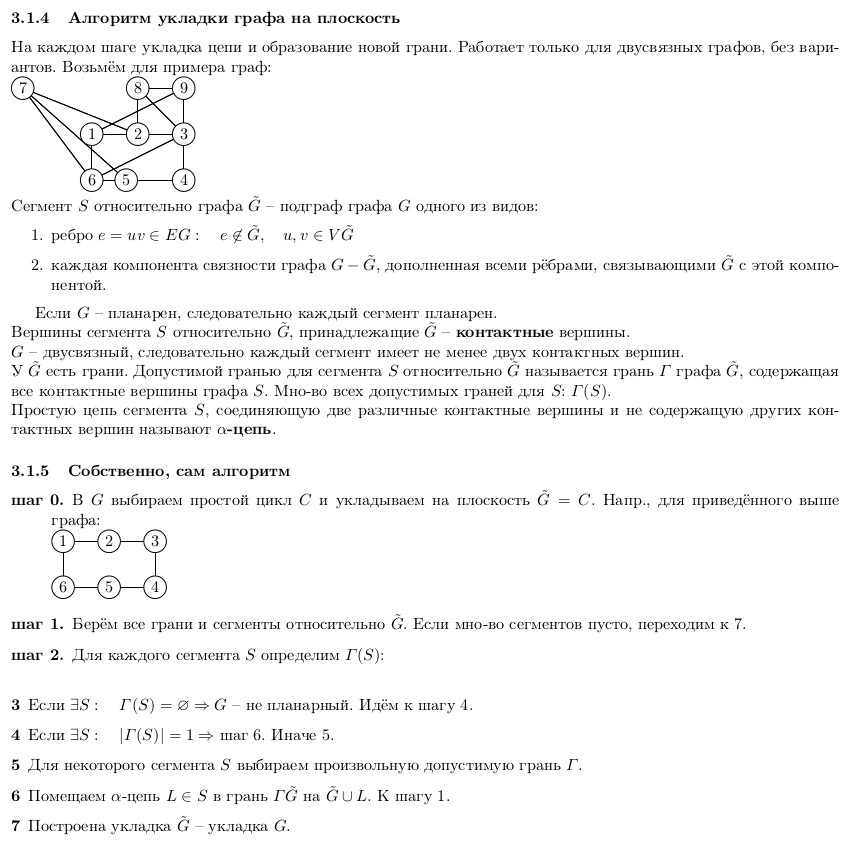
\includegraphics[width=600pt]{6}\\\\\\\\\\\\\\\\\\\\
		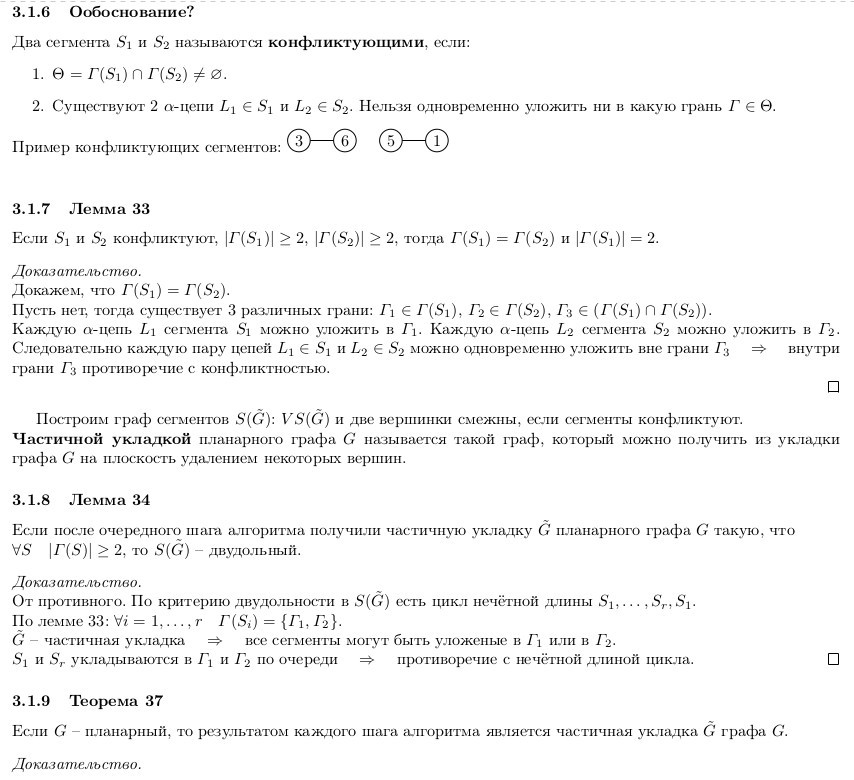
\includegraphics[width=600pt]{7}\\
		инд. по числу шагов:\\
		Шаг 0 — укладка цикла\\
		...\\
		...\\
		Шаг $n$ — $\widetilde{G}$ — частичная укладка; если $\exists$ $Г(S)$ = $\emptyset$ $\Rightarrow$ $G$ не планарен\\
		Если $\exists S:$ $|Г(S)| = 1$\\
		В исходной укладке $G$ S уложен в $Г:$ $Г(S) = \{Г\}$\\ $\Rightarrow$ укладка $\alpha$-цепи из $S$ в $Г$ $\Rightarrow$ получим частичную укладку\\
		Теперь пусть $Г(S) \geqslant 2$ $\forall S$\\
		Рассм. $S(\widetilde{G})$ — он двудольный. Берём произвольную вершину $S$. Если $S$ изолированная вершина, то $S$ ни с кем не конфликтует $\Rightarrow$ укладка $\alpha$-цепи из $S$ не мешает частичной укладке $\Rightarrow$ всё хорошо\\
		Если $S$ не изолированная вершина $\Rightarrow$ $S$ лежит в непустой компоненте связности графа S($\widetilde{G}$). В этой к.с. все сегменты содержат 2 одинаковые грани.\\
		$S_1,\dotsc,S_t$ — вершины этой к.с.\\
		По лемме 33 $\forall i$ $Г(S) = \{Г_1, Г_2\}$\\
		По лемме 34 $S(\widetilde{G})$ — двудольный\\
		И получается в исходной укладке $G$ на плоскость сегменты из 1-ой доли уложены в $Г_1$, из др. доли в $Г_2$\\
		И если в ней поменять местами $Г_1$ и $Г_2$ то получим укладку $G$ на плоскости\\
	\qedsymbol
\section{Правильная раскраска вершин графа. Верхние оценки хроматического числа. Теорема Брукса }
\subsection{Правильная раскраска вершин графа.}
	$G = (V,E)$\\
	$\varphi:V \to \{c_1,\dotsc,c_t\}$ — раскраска вершин разбиения $V = V_1 \sqcup \dotsb \sqcup V_t$; $V_i$ — мн-во вершин цвета $c_i$\\
	Раскраска $\varphi$ правильная, если:\\
	$xy \in E \Rightarrow \varphi(x) \neq \varphi(y) \Rightarrow \forall i \quad V_i$ — независимое мн-во
\subsection{Верхние оценки хроматического числа.}
\subsubsection{Оценка 1}
	$G$ — $(n,m)$-граф $\Rightarrow$ $\chi(G) \leqslant \frac{1}{2} + \sqrt{2m + \frac{1}{4}}$\\
	\textbf{Доказательство:}\\
		$\forall$ пары цветов $\exists$ ребро на концах которого вершины этих цветов (из леммы о том, что в правильной раскраске для $\forall$ цвета $\exists$ вершина этого цвета, в окружении которой есть вершины всех остальных цветов)	
		$\Rightarrow$ $m \geqslant \binom{\chi(G)}{2}$\\
	\qedsymbol
\subsubsection{Оценка 2}
	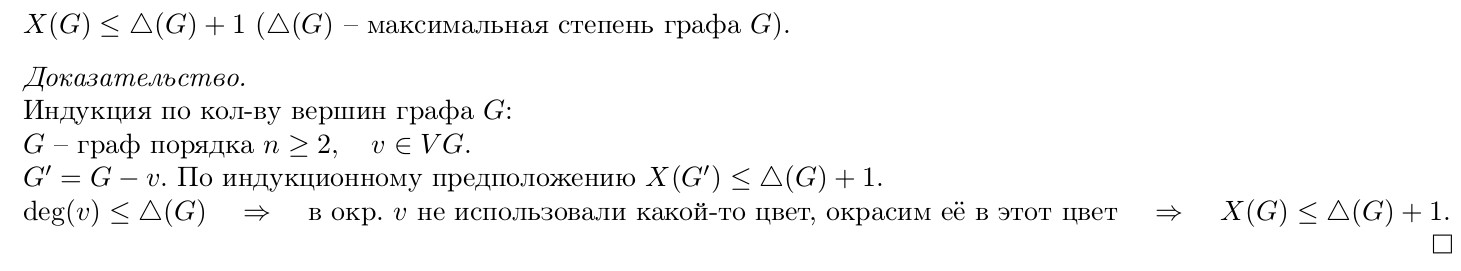
\includegraphics[width=550pt]{8}
\subsection{Теорема Брукса}
	$\forall$ связного графа, не явл. $K_n, C_{2n + 1} \quad \chi(G) \leqslant \Delta(G)$\\
	\textbf{Доказательство:}\\
		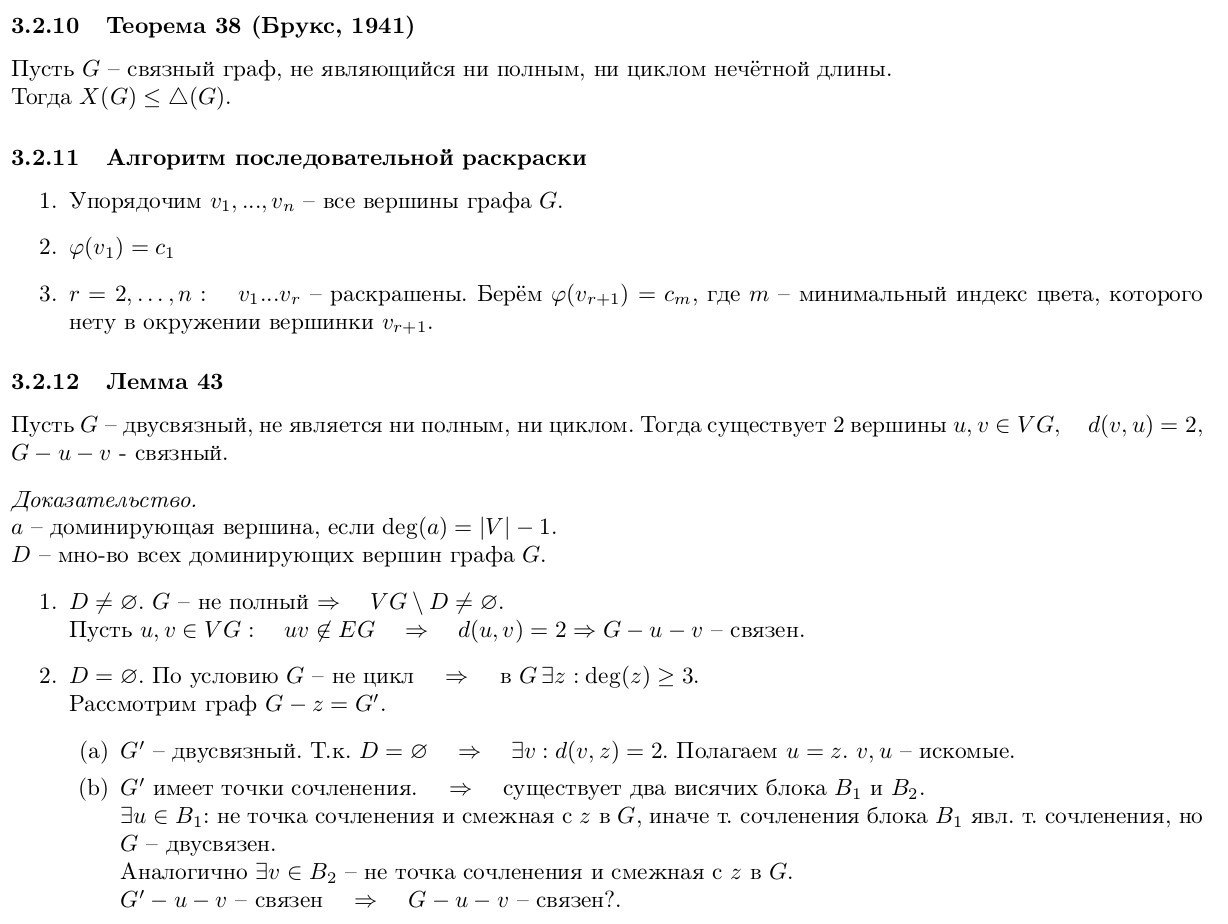
\includegraphics[width=600pt]{9}\\
		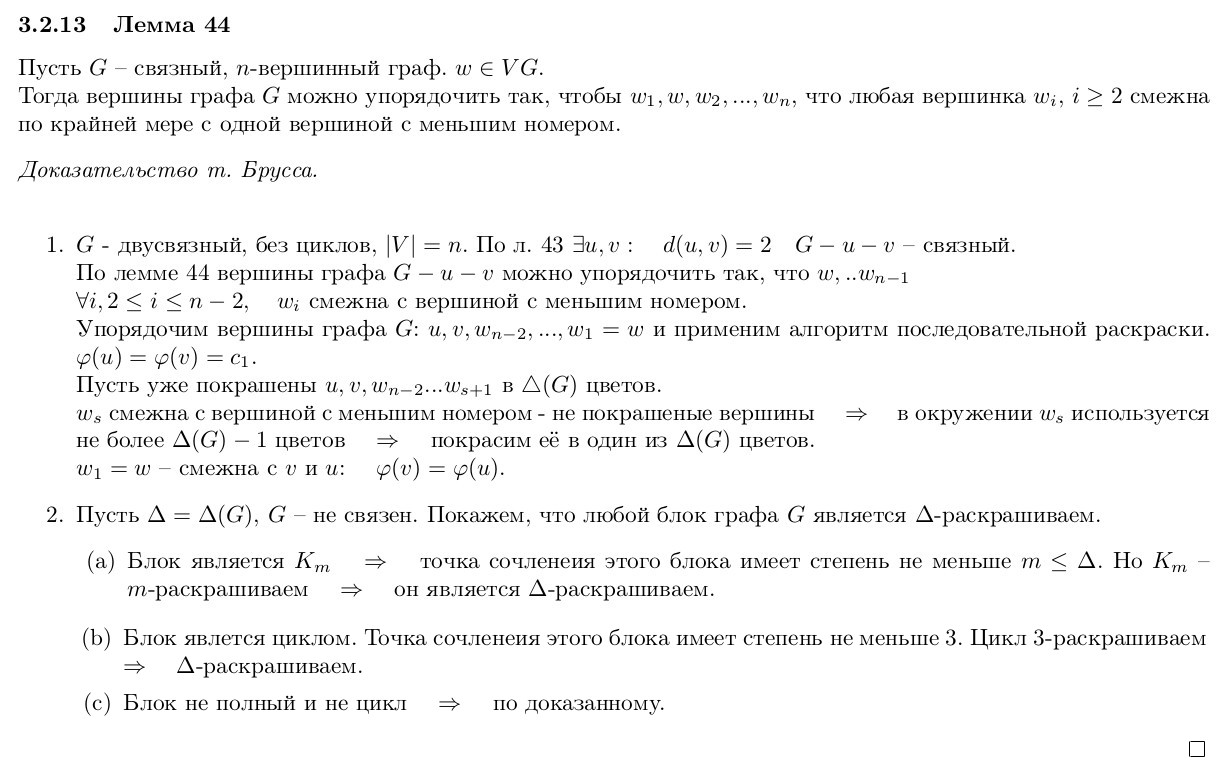
\includegraphics[width=600pt]{10}
	\qedsymbol

\section{Правильная раскраска вершин графа. Нижние оценки хроматического числа. Теорема о существовании графов без треугольников с большим хроматическим числом.}
\subsection{Правильная раскраска вершин графа.}
	$G = (V,E)$\\
	$\varphi:V \to \{c_1,\dotsc,c_t\}$ — раскраска вершин разбиения $V = V_1 \sqcup \dotsb \sqcup V_t$; $V_i$ — мн-во вершин цвета $c_i$\\
	Раскраска $\varphi$ правильная, если:\\
	$xy \in E \Rightarrow \varphi(x) \neq \varphi(y) \Rightarrow \forall i \quad V_i$ — независимое мн-во
\subsection{Нижние оценки хроматического числа.}
	1) $\chi(G) = \chi$\\
	$G = (V, E)$\\
	$V = V_1 \sqcup \dotsb, \sqcup V_\chi$\\
	$V_i$ — независимое мн-во $\forall i$\\
	$|V_i| < \alpha_0(G) \quad \forall i$\\
	$|VG| = \sum|V_i| \leqslant \alpha_0(G) * \chi(G)$\\
	$\Downarrow$\\
	$\chi(G) \geqslant \frac{|VG|}{\alpha_0(G)}$\\
	2) $\chi(G) \geqslant \alpha_0(\bar{G})$\\
	3) $\chi(G) \geqslant t$\\
	$t$ — мощность наиб. клики в G\\
\subsection{Теорема о существовании графов без треугольников с большим хроматическим числом.}
%	Существуют примеры графов $G_2,G_3,G_4,\dotsc$ т.ч.:
%	1) В $G_i$ нет треугольников\\
%	2) $\chi(G_i) = i$\\
%	поиск:\\
%	$G_2 = K_2$\\
%	$G_i = (V_i,E_i)$\\
%	$G_{i+1}$: берём $G_i$ и дубоируем каждую вершину. Т.е. если есть вершина смежная с $v1,\dotsc,v_k$, то создаём вершину тоже смежную с $v_1,\dotsc,v_k$\\
%	$V_i'$ — множество дублей; $w_i$ — новая: $N_{G_{i+1}}(w_i) = V_i'$\\
	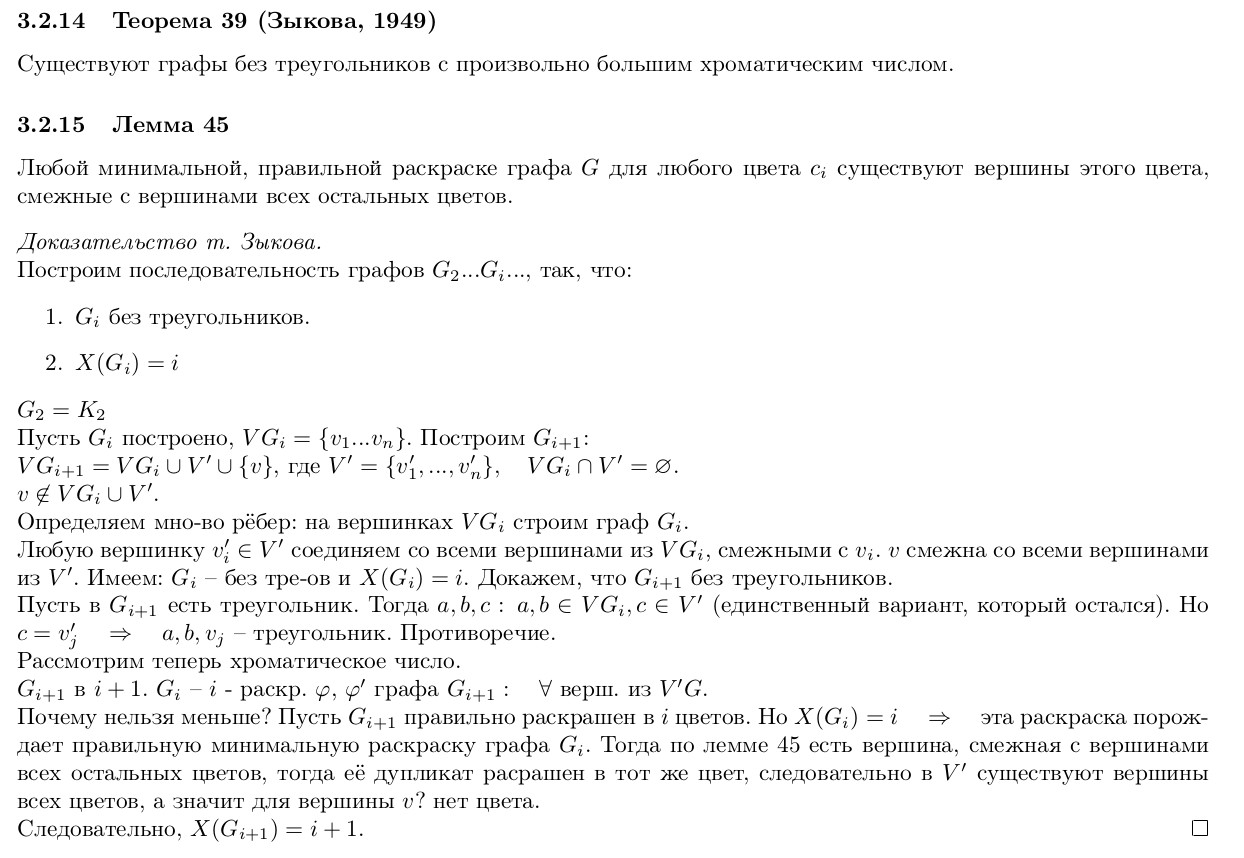
\includegraphics[width=600pt]{11}
\section{Раскраски планарных графов. Теорема о четырех красках. Теорема Хивуда.}
\subsection{Теорема о четырех красках.}
	$\forall$ планарный граф 4-раскрашиваем\\
	\textbf{Доказательство:}\\
	б/д\\
	\qedsymbol
\subsection{Теорема Хивуда.}
	$\forall$ планарный граф 5-раскрашиваем\\
	\textbf{Доказательствой:}\\
		Индукция по числу вершин $n = |VG|$\\
		При $n \leqslant 5$ теор. верна\\
		переход\\
		G — планарный граф на $n > 5$ вершинах\\
		В $G$ $\exists$ вершина $x$ т.ч. $deg x \leqslant 5$ (иначе, в графе был бы подграф $K_{3,3}$)\\
		$G' = G - x$; по инд. предположению $\exists$ прав. раскр. $\varphi$ в 5 цветов\\
		Возвращаем вершину $x$\\
		Если $deg x < 5$, то всё хорошо, перекрашиваем в свободный цвет\\
		Если $deg x = 5$ и в окр. $x$ есть одинаковые цвета, то всё хорошо\\
		Если $deg x = 5$  и в окр. $x$ есть все 5 цветов\\
		$c_i, c_j$ — 2 цвета. рассмотрим вершины этих цветов\\
		$G_{i,j}$ — подграф графа $G$ порождённый вершинами $c_i$ и $c_j$\\
		Рассмотрим $G_{1,3}$. Если $y_1$ и $y_3$ в разных к. с. $G_{1,3}$, то 1 к. с. графа $G_{1,3}$ перекрашиваем и освобождаем цвет для $x$\\
		Если $y_1$ и $y_3$ в одной к.с. графа $G_{1,3}$, то $\exists$ $(y_1,y_3)-$цепь из вершин цвета $с_1$ и $c_3$. Тогда рассмотрим вершины $y_2$ и $y_4$. Они в разных к.с. графа $G_{2,4}$ т.к. граф $G$ плоский и $(y_2,y_4)$-цепь должна пересекать $(y_1,y_3)$-цепь\\
		\qedsymbol 
\section{Правильная раскраска ребер графа. Хроматический индекс. Теорема Кёнига о хроматическом индексе двудольных графов.}
\subsection{Правильная раскраска ребер графа.}
	$\varphi: EG \to \{c_1,\dotsc,c_t\}$ — раскраска рёбер в $t$ цветов\\
	$\varphi$ 	— правильная рёберная раскраска, если $e$ и $h$ смежны $\Rightarrow$ $\varphi(e) \neq \varphi(h)$\\
\subsection{Хроматический индекс.}
	$G$ — рёберно $t$-хроматический, если $G$ рёберно $t$-раскрашиваемый и не является рёберно\\$(t-1)$-раскрашиваемым.\\
	$G$ — рёберно $t$-хроматический $\Rightarrow$ t — рёберное хроматическое число (хроматический индекс) $\chi'(G)$
\subsection{Теорема Кёнига о хроматическом индексе двудольных графов.}
	$\forall$ двудольного графа $G$: $\chi'(G) = \Delta(G)$\\
	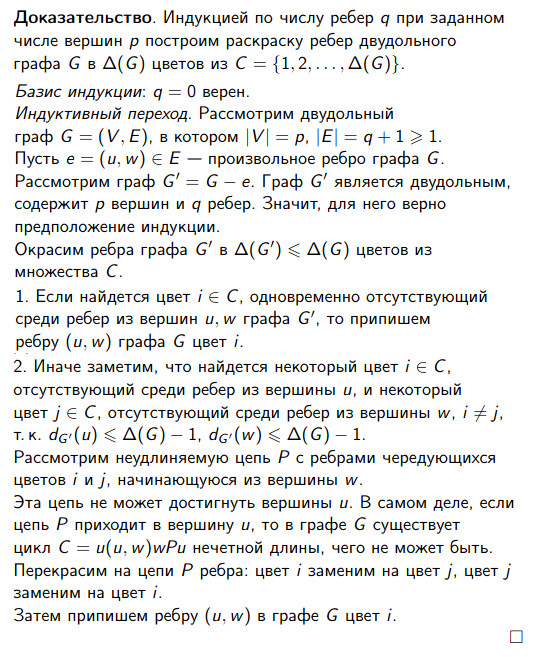
\includegraphics[width=400pt]{12}\\

\section{Теорема Визинга о хроматическом индексе графа (без доказательства). Хроматический индекс полного графа.}
\subsection{Теорема Визинга о хроматическом индексе графа (без доказательства).}
	$\forall$ графа $G$: $\Delta(G) \leqslant \chi'(G) \leqslant \Delta(G) + 1$
\subsection{Хроматический индекс полного графа.}
	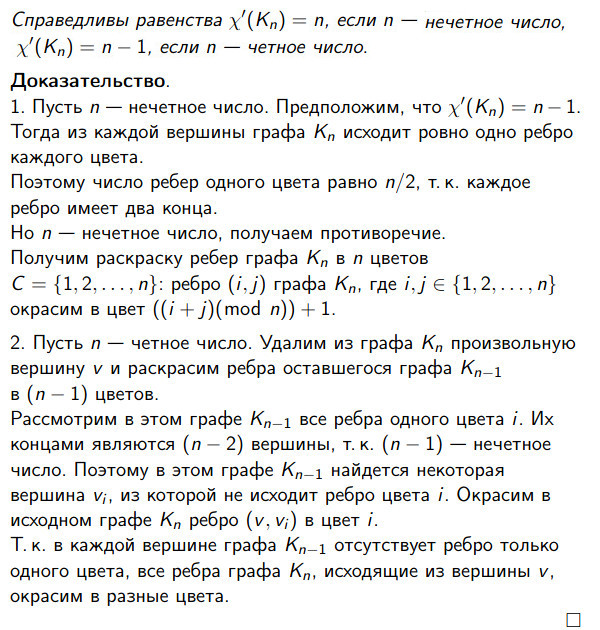
\includegraphics[width=400pt]{13}

\section{Теорема Рамсея для графов.}
	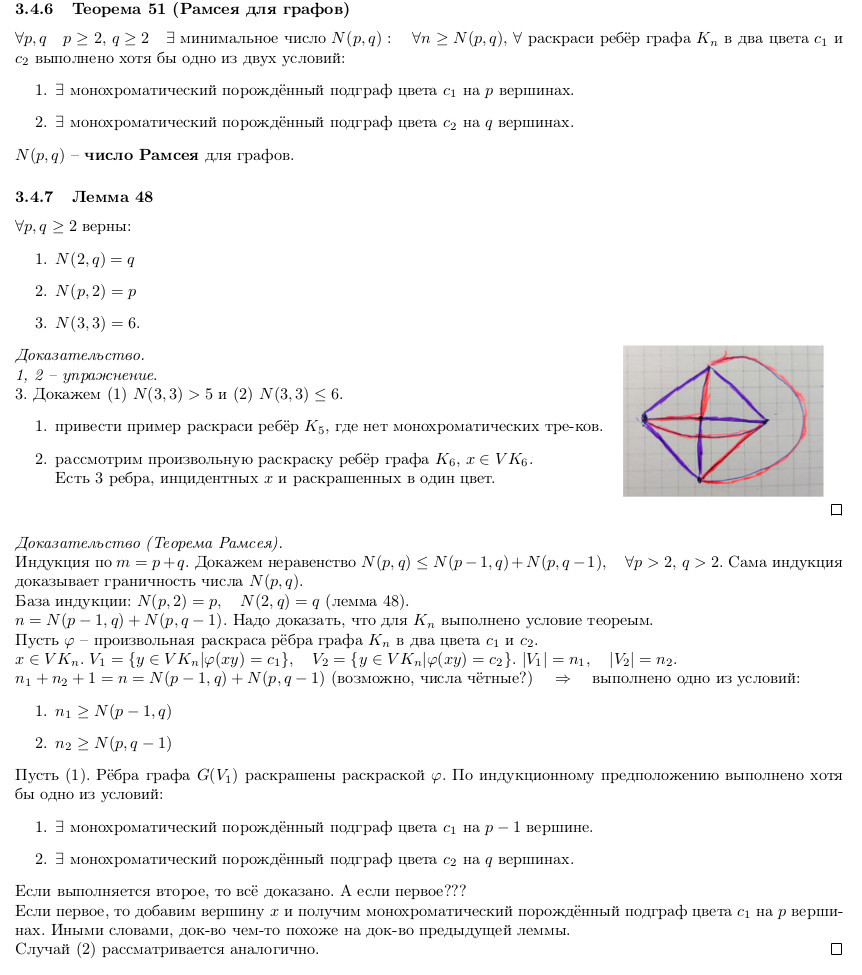
\includegraphics[width=500pt]{14}

\section{Правильная раскраска ребер графа. Хроматический индекс. Теорема о хроматическом индексе полного графа.}
	\subsection{Правильная раскраска ребер графа.}
	$\varphi: EG \to \{c_1,\dotsc,c_t\}$ — раскраска рёбер в $t$ цветов\\
	$\varphi$ 	— правильная рёберная раскраска, если $e$ и $h$ смежны $\Rightarrow$ $\varphi(e) \neq \varphi(h)$\\
\subsection{Хроматический индекс.}
	$G$ — рёберно $t$-хроматический, если $G$ рёберно $t$-раскрашиваемый и не является рёберно\\$(t-1)$-раскрашиваемым.\\
	$G$ — рёберно $t$-хроматический $\Rightarrow$ t — рёберное хроматическое число (хроматический индекс) $\chi'(G)$
\subsection{Теорема о хроматическом индексе полного графа.}
	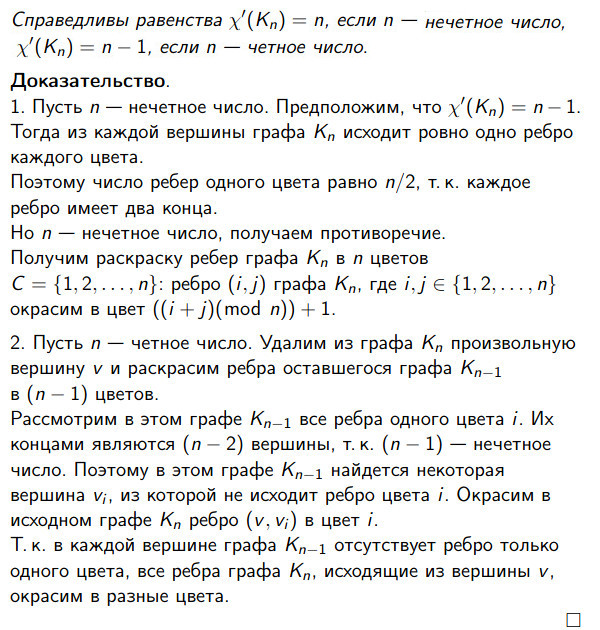
\includegraphics[width=400pt]{13}

\section{Булева функция. Существенные и фиктивные переменные. Теорема о числе булевых функций, существенно зависящих от n переменных.}
\subsection{Булева функция.}
	Фуекция вида $f: \{0,1\}^n \to \{0,1\}$ — булева
\subsection{Существенные и фиктивные переменные.}
	Переменная $x_i$ функции $f(x_1,\dotsc,x_n)$ — существенная, если $\exists \text{ набор переменных } \alpha_1,\dotsc,\alpha_n$ т.ч.\\ $f(\alpha_1,\dotsc,\alpha_n) \neq f(\alpha_1,\dotsc,\bar{\alpha_i},\dotsc,\alpha_n)$\\
	иначе — фиктивная
\subsection{Теорема о числе булевых функций, существенно зависящих от n переменных.}
	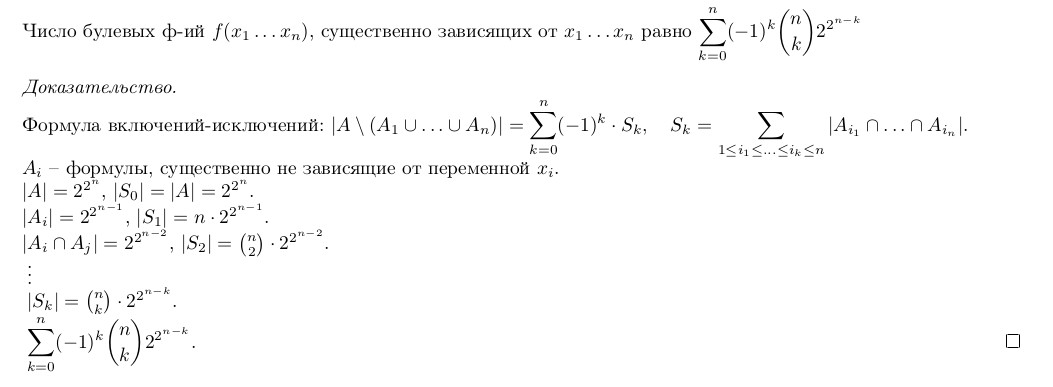
\includegraphics[width=560pt]{15}

\section{Формула. Функция, которую реализует формула. Эквивалентные формулы. Основные эквивалентности.}
\subsection{Формула.}
	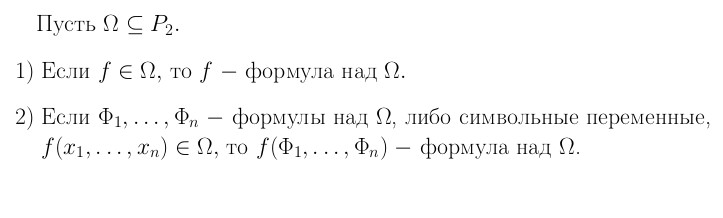
\includegraphics[width=500pt]{16}
\subsection{Функция, которую реализует формула.}
	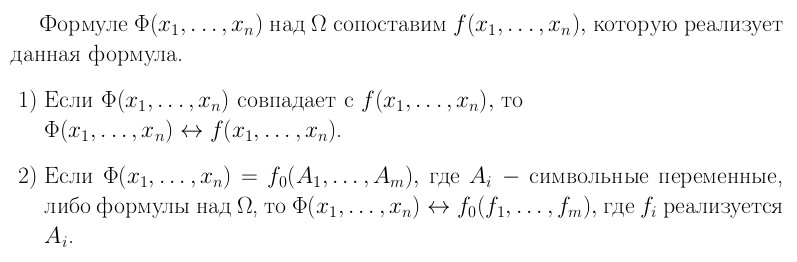
\includegraphics[width=500pt]{17}
\subsection{Эквивалентные формулы.}
	Формулы эквивалентны, если они реализуют равные функции
\subsection{Основные эквивалентности.}
	$x_1 \circ x_2$ — любая из ф-ций $x_1 \	 x_2$; $x_1 \vee x_2$; $x_1 \oplus x_2$
	\begin{enumerate}
		\item $x_1 \circ x_2 = x_2 \circ x_1$
		\item $x_1 \circ (x_2 \circ x_3) = (x_1 \circ x_2) \circ x_3$
		\item $(x_1 \vee x_2) \& x_3 = (x_1 \& x_3) \vee (x_2 \& x_3)$
		\item $(x_1 \& x_2) \vee x_3 = (x_1 \vee x_3) \& (x_2 \vee x_3)$
		\item $(x_1 \oplus x_2) \& x_3 = (x_1 \& x_3) \oplus (x_2 \& x_3)$
		\item $\bar{\bar{x}} = x$
		\item $\bar{x_1 \& x_2} = \bar{x_1} \vee \bar{x_2}$
		\item $\bar{x_1 \vee x_2} = \bar{x_1} \& \bar{x_2}$
		\item $x_1 \& (x_1 \vee x_2) = x_1$
		\item $x_1 \vee (x_1 \& x_2) = x_1$
		\item $x \& \bar{x} = 0$
		\item $x \vee \bar{x} = 1$
		\item $x \& x = x$
		\item $x \vee x = x$
		\item $x \oplus x = 0$
		\item $x \oplus 1 = \bar{x}$
		\item $x \oplus \bar{x} = 1$
		\item $x \oplus 0 = x$
		\item $x \& 0 = 0$
		\item $x \vee 0 = x$
		\item $x \& 1 = x$
		\item $x \vee 1 = 1$
	\end{enumerate}
	\textbf{Доказательство:}\\
	Нарисовать таблицы для левых и правых частей\\
	\qedsymbol
\section{Теорема о разложении функций по переменным. Совершенная дизъюнктивная нормальная форма. Совершенная конъюнктивная нормальная форма. Двойственная функция. Принцип двойственности.}
\subsection{Теорема о разложении функций по переменным.}
	Пусть $f(x_1,\dotsc,x_n) \in P_2, \quad 1 \leqslant k \leqslant n$\\
	Тогда $f(x_1,\dotsc,x_n) = \displaystyle\bigvee_{\sigma_1,\dotsc,\sigma_k \in \{0,1\}^k}x_1^{\sigma_1}\dotsm x_k^{\sigma_k} f(\sigma_1, \dotsc, \sigma_k, x_{k+1}, \dotsc, x_{n})$ (*)\\
	\textbf{Доказательство:}\\
		Если подставить конкретные значения, то в правой части останется только одна конъюнкция, и оставшаяся конъюнкция совпадёт с левой частью\\ 
	\qedsymbol
\subsection{Совершенная дизъюнктивная нормальная форма.}
	Разложение ф-ции отличной от $0$ вида (*) при $k=n$ называется СДНФ (совершенная дизъюнктивная нормальная форма)
\subsection{Совершенная конъюнктивная нормальная форма.}
	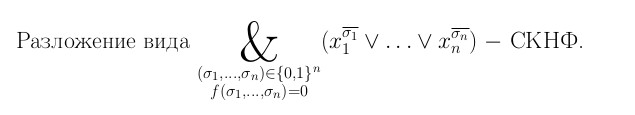
\includegraphics[width=400pt]{18}
\subsection{Двойственная функция.}
	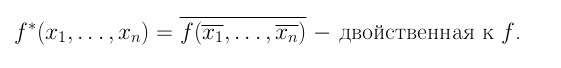
\includegraphics[width=400pt]{19}
\subsection{Принцип двойственности.}
	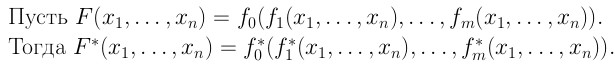
\includegraphics[width=400pt]{20}

\section{Замкнутое, полное множества булевых функций. Теорема о полноте двух систем.}
\subsection{Замкнутое, полное множества булевых функций.}
	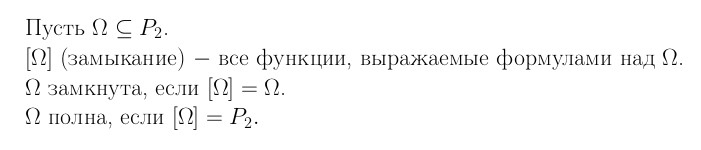
\includegraphics[width=400pt]{21}
\subsection{Теорема о полноте двух систем.}
	$\Omega_1, \Omega_2 \subseteq P_2$\\
	$\Omega_1$ — полна, и $\forall$ ф-я из $\Omega_1$ выражается ф-лой над $\Omega_2$, тогда $\Omega_2$ — полна\\
	\textbf{Доказательство:}\\
		$[\Omega_1] = P_2 \quad \Omega_1 \subset [\Omega_2]$\\
		$P_2 = [\Omega_1] \subseteq [[\Omega_2]] = [\Omega_2] \subseteq P_2$\\
		$\Downarrow$\\
		$[\Omega_2] = P_2$\\
	\qedsymbol

\section{Полином Жегалкина. Теорема Жегалкина. Способы построения полинома Жегалкина.}
\subsection{Полином Жегалкина.}
	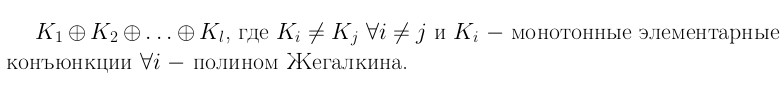
\includegraphics[width=500pt]{22}
\subsection{Теорема Жегалкина.}
	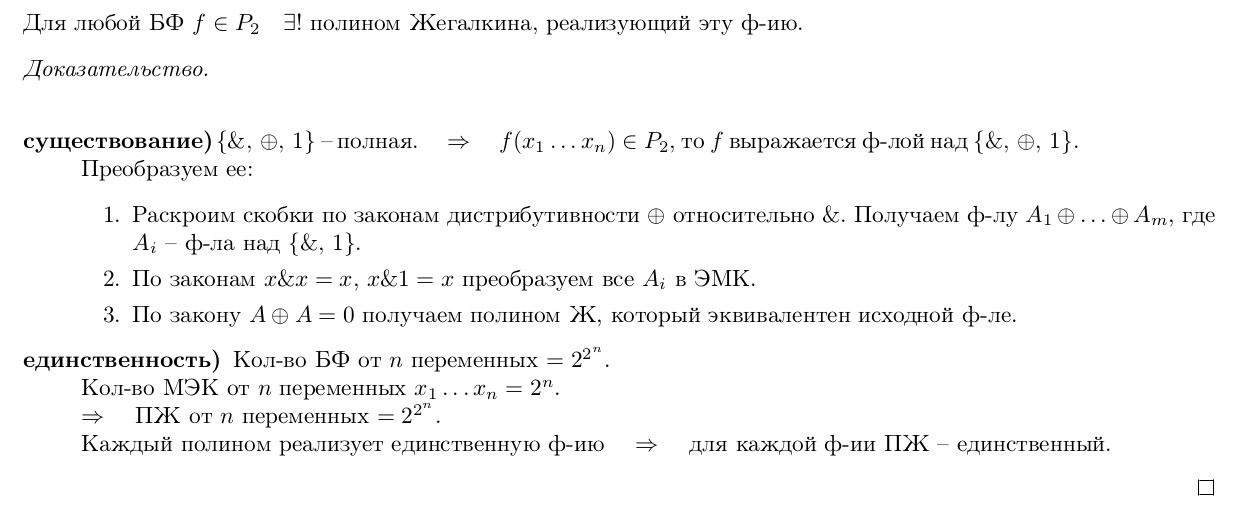
\includegraphics[width=550pt]{23}
\subsection{Способы построения полинома Жегалкина.}
	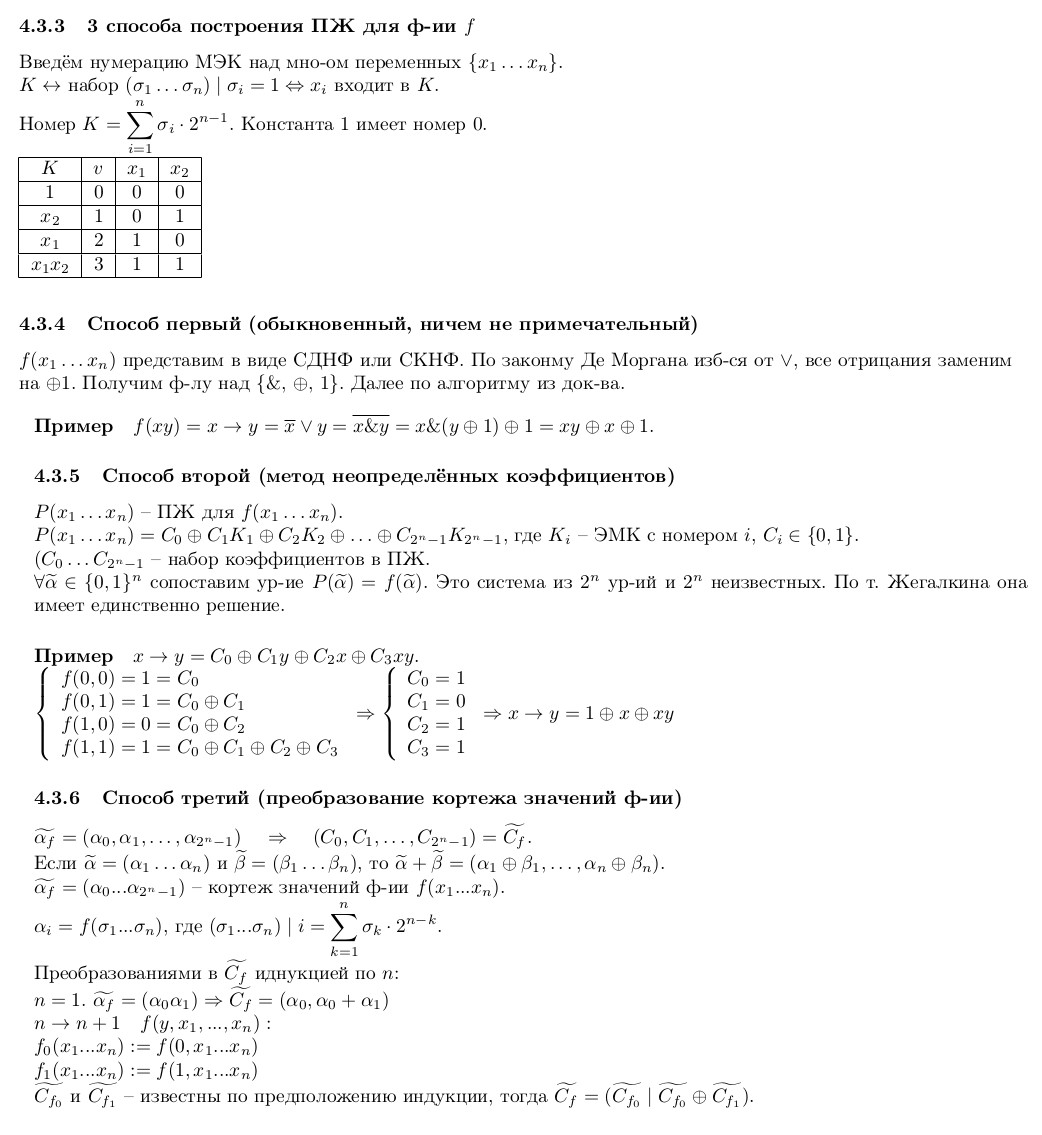
\includegraphics[width=550pt]{24}

\section{Основные замкнутые классы булевых функций. Предполные классы.}
\subsection{Основные замкнутые классы булевых функций.}
	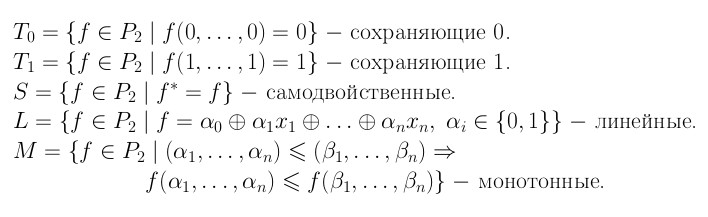
\includegraphics[width=370pt]{25}\\
	$T_0, T_1, S, L, M$ — замкнуты\\
	\textbf{Доказательство:}\\
		1. $f_0, \dotsc, f_m \in T_0$\\
		Рассм. $F(0,\dotsc,0) = f_0(f_1(0,\dotsc,0),\dotsc f_m(0,\dotsc,0)) = f_0(0,\dotsc,0) = 0$\\
		2. $f_0, \dotsc, f_m \in T_1$\\
		Аналогично\\
		3. $f_0, \dotsc, f_m \in S$\\
		$F^*(x_1,\dotsc,x_n) \underset{\text{принцип двойственности}}{=} f_0^*(f_1^*(x_1,\dotsc,x_n),\dotsc f_m^*(x_1,\dotsc,x_n)) = f_0(f_1(x_1,\dotsc,x_n),\dotsc f_m(x_1,\dotsc,x_n)) = F(x_1,\dotsc,x_n)$\\
		4. $f_0, \dotsc, f_m \in L$\\
		$L = [\{\oplus, 1\}]$ $\Rightarrow$ L замкнуто\\
		5. $f_0, \dotsc, f_m \in M$\\
		$(\alpha_1,\dotsc,\alpha_n) \leqslant (\beta_1,\dotsc,\beta_n) \quad 1 \leqslant i \leqslant m$\\
		$\Downarrow$\\
		$(f_1(\alpha_1,\dotsc,\alpha_n),\dotsc,f_m(\alpha_1,\dotsc,\alpha_n)) \leqslant (f_1(\beta_1,\dotsc,\beta_n),\dotsc,f_m(\beta_1,\dotsc,\beta_n))$\\
		$\Downarrow$ ($f_0 \in M$)\\
		$f_0(f_1(\alpha_1,\dotsc,\alpha_n),\dotsc,f_m(\alpha_1,\dotsc,\alpha_n)) \leqslant f_0(f_1(\beta_1,\dotsc,\beta_n),\dotsc,f_m(\beta_1,\dotsc,\beta_n))$\\
		$\Downarrow$\\
		$F(\alpha_1,\dotsc,\alpha_n) \leqslant F(\beta_1,\dotsc,\beta_n)$\\
	\qedsymbol
\subsection{Предполные классы.}
	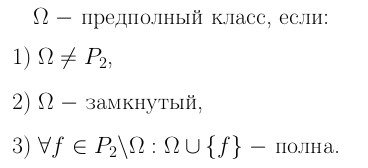
\includegraphics[width=250pt]{26}
\section{Теорема Поста.}
Леммы, необходимые для доказательства теоремы:
\subsection{Лемма о несамодвойственной ф-ции}
	$f \notin S$ $\Leftrightarrow$ $0,1 \in [\{f, \bar{x}\}]$\\
	\textbf{Доказательство:}\\
		$\Rightarrow$) $f \in S$ $\Leftrightarrow$ $\forall$ ($\alpha_1,\dotsc,\alpha_n$) $\quad$ $f(\alpha_1,\dotsc,\alpha_n) = \overline{f(\overline{\alpha_1},\dotsc,\overline{\alpha_n})}$\\
		$g(x) = f(x^{\alpha_1},\dotsc,x^{\alpha_n})$\\
		$g(0) = f(0^{\alpha_1},\dotsc,0^{\alpha_n}) = f(\overline{\alpha_1},\dotsc,\overline{\alpha_n}) = \*f(\alpha_1,\dotsc,\alpha_n) = f(1^{\alpha_1},\dotsc,1^{\alpha_n}) = g(1)$\\
		$\Downarrow$\\
		$g(x)$	— const\\
		$\Leftarrow$) Дано $0,1 \in [\{f, \bar{x}\}]$\\
		От противного\\
		Пусть $f \in S$ $\Rightarrow$ $\{f, \bar{x}\} \subseteq S$ $\overset{\text{S — замкнут}}{\Rightarrow}$ $[\{f, \bar{x}\}] \subseteq S$\\
		Но $0,1 \notin S$\\
		Противоречие\\
	\qedsymbol
\subsection{Лемма о немонотонной ф-ции}
	$f \notin M$ $\Leftrightarrow$ $\bar{x} \in [\{f, 0,1\}]$\\
	\textbf{Доказательство:}\\
		$\Leftarrow$) Аналогично прошлой лемме\\
		$\Rightarrow$)
		Пусть $f(x_1,\dotsc,x_n) \notin M$\\
		$\Downarrow$\\
		$\exists (\alpha_1,\dotsc,\alpha_n) \leqslant (\beta_1,\dotsc,\beta_n)$ т.ч.$f(\alpha_1,\dotsc,\alpha_n) > f(\beta_1,\dotsc,\beta_n)$\\
		$\Downarrow$\\
		$f(\alpha_1,\dotsc,\alpha_n) = 1$\\
		$f(\beta_1,\dotsc,\beta_n) = 0$\\
		Рассм. $g(x)$ получаемая из $f(x_1,\dotsc,x_n)$ подставлением на место $x_i$:
		$\begin{cases}
			0; \text{ если } \alpha_i = \beta_i = 0\\
			1; \text{ если } \alpha_i = \beta_i = 1\\
			x_i; \text{ если } \alpha_i \neq \beta_i = 1 \Leftrightarrow \alpha_1=0, \beta_i=1
		\end{cases}$\\
		$g(0) = f(\alpha_1,\dotsc,\alpha_n) = 1$\\
		$g(1) = f(\beta_1,\dotsc,\beta_n) = 0$\\
		$\Downarrow$\\
		$g(x) = \overline{x}$\\
	\qedsymbol
\subsection{Лемма о нелинейной ф-ции}
	$f \notin L$ $\Leftrightarrow$ $x \& y \in [\{f, \overline{x},0, 1\}]$\\
	\textbf{Доказательство:}\\
		$\Leftarrow$) Аналогично прошлой лемме\\
		$\Rightarrow$)
		Пусть $f(x_1,\dotsc,x_n) \notin L$\\
		$K = x_1\dotsm x_r$\\
		Если что, переменные перенумеруем. Но выберем такое $r$, что
		у $f(x_1,\dotsc,x_r,0,\dotsc,0)$ в полиноме Жегалкина ровно одно слагаемое имеет ранг больше 1\\
		$f(x_1,x_2,1\dotsc,1,0,\dotsc,0) = x_1x_2 \oplus \alpha x_1 \oplus \beta x_2 \oplus \gamma$\\
		$f(x_1 \oplus \beta,x_2 \oplus \alpha,1\dotsc,1,0,\dotsc,0) = (x_1 \oplus \beta)(x_2 \oplus \alpha) \oplus \alpha (x_1 \oplus \beta) \oplus \beta (x_2 \oplus \alpha) \oplus \gamma = x_1x_2 \oplus \alpha \beta \oplus \gamma \in \{x_1x_2, \overline{x_1x_2}\}$\\
		Если получили $\overline{x_1x_2}$, то $\overline{\overline{x_1x_2}} = x_1x_2$\\
	\qedsymbol
\subsection{Теорема Поста.}
	Сист. б.ф. $\Omega \subseteq P_2$ полна $\Leftrightarrow$ она не лежит целиком ни в из классов $T_0, T_1, S, L, M$\\
	\textbf{Доказательство:}\\
		$\Rightarrow$) $\Omega$ — полна $\Rightarrow$ функциями из $\Omega$ можно выразить штрих Шеффера.\\
		Т. к. классы $T_0, T_1, L, S, M$ замкнуты и штрих шеффера не принадлежит ни одному из этих классов. То Штрих шеффера выражается функциями не из этих классов $\Rightarrow$ $\Omega$ не может лежать целиком ни в одном из этих классов\\
		$\Leftarrow$) $\Omega \nsubseteq T_0 \Rightarrow \exists f_0 \in \Omega \setminus T_0$\\
		аналогично:\\
		$\exists f_1 \in \Omega \setminus T_1$\\
		$\exists f_S \in \Omega \setminus S$\\
		$\exists f_L \in \Omega \setminus L$\\
		$\exists f_M \in \Omega \setminus M$\\
		Рассм. $\Omega' = \{f_0, f_1, f_S, f_L, f_M\}$\\
		Хотим показать, что $x \& y, \overline{x} \in [\Omega']$\\
		Шаг 1. Покажем что $0,1,\overline{x} \in [\Omega']$\\
		$\varphi_1(x) = f_0(x,\dotsc,x)$\\
		$\varphi_2(x) = f_1(x,\dotsc,x)$\\
		$\varphi_1(0) = f_0(0,\dotsc,0) = 1 \Rightarrow \varphi_1 \in \{1, \overline{x}\}$\\
		$\varphi_2(1) = f_1(1,\dotsc,1) = 0 \Rightarrow \varphi_2 \in \{0, \overline{x}\}$\\
		Если $\varphi_1(x) \neq \overline{x}$ и $\varphi_2(x) \neq \overline{x}$. Тогда $\varphi_1(x) = 1, \varphi_2(x) = 0$\\
		Тогда по лемме о немонотонной ф-ции $\overline{x} \in [f_m, 0, 1]$\\
		В противном случае $\overline{x} \in \{\varphi_1, \varphi_2\}$\\
		Т.о. $\overline{x}$ получили\\
		По лемме о несамодвойственной ф-ции $0,1 \in [\{f_s, \overline{x}\}]$\\
		Показали\\
		Шаг 2\\
		По лемме о нелинейной ф-ции\\
		$x_1, x_2 \in [\{f_L, 0, 1, \overline{x}\}]$\\
		В итоге мы получили\\
		$x \& y \in [\Omega']$\\
		$\Downarrow$ по теореме о полноте двух систем\\
		$\Omega' полна$ $\Rightarrow$ $\Omega$ полна\\
	\qedsymbol

\section{Минимизация ДНФ. Способы построения сокращенной ДНФ.}
\subsection{Минимизация ДНФ.}
\subsubsection{Элементарная конъюнкция}
	элементарная конъюнкция ранаг r\\
	$K = x_{i_1}^{\sigma_{i_1}} \dotsb x_{i_r}^{\sigma_{i_r}}$\\
	Эл. конъюнкция ранга $0$ 	— $K = 1$ 
\subsubsection{ДНФ}
	$K_1 \vee \dotsb \vee K_s$; $K_i \neq K_j$ $i \neq j$\\
	$\forall 1 \leqslant i \leqslant s$ $K_i$ — элементарная конъюнкция
\subsection{Мин. ДНФ}
	ДНФ $D$ наз-ся минимальным ДНФ ф-ции $f$, если она имеет мин. сумму рангов вход. в неё эл. конъюнкций среди всех ДНФ реализующих ф-цию $f$
\subsection{Теорема}
	Сокращённая ДНФ монотонрой ф-ции $f$ не содержит отрицаний переменных и явл. её ед. мин. ДНФ\\
	\textbf{Доказательство:}\\
		$f \in M$\\
		$f = K_1 \vee \dotsb \vee K_s$ — сокр. ДНФ\\
		$K_i = x_{i_1}x_{i_2}\dotsm x_{i_t}\overline{x_{i_t + 1}}\dotsm \overline{x_{i_r}}$\\
		$f$ принимает значение 1 на всех кортежах (наборах):
		$(\alpha_1,\dotsc,\alpha_n): \alpha_{i_1} = \alpha_{i_2} = \dotsc = \alpha_{i_t} = 1$\\
		$\alpha_{i_t + 1} = \dotsc = \alpha_{i_r} = 1$\\
		из монотонности\\
		$\Rightarrow$ и на всех кортежах $(\beta_1,\dotsc,\beta_n)$: $\beta_{i_1} = \dotsc, = \beta_{i_t} = 1$\\
		$K' = x_{i_1}\dotsm x_{i_t}$ — импликанта ф-ции\\
		$K < K' \leqslant f$ $\Rightarrow$ K не простая\\
		Противоречие\\
	\qedsymbol
\subsection{Способы построения сокращенной ДНФ.}
	3 операции:
	\begin{enumerate}
		\item склеивание $xK \vee \overline{x}K = K$
		\item поглощение $K_1 \vee K_1K2 = K_1$
		\item обощ. склеивание $xK_1 \vee \overline{x}K_2 = xK_1 \vee \overline{x}K_2 \vee K_1K_2$
	\end{enumerate}
	Алгоритмы:
	\textbf{метод Нельсона} (из КНФ)\\
	раскрываем все скобки, поглощение, убираем дублирование\\
	\textbf{Метод Квайна} (из СДНФ)\\
	все пары проверяем на склейк $\Rightarrow$ все пары рёбер проверяем на склейку $\Rightarrow$ получаем грани размерности 2 и т.д. пока можем $\Rightarrow$ Поглощение\\
	\textbf{Метод Блейка}\\
	Пока можем обобщ. склеивание, потом поглощение\\

\section{Схема из функциональных элементов. Система функций, реализуемая схемой из функциональных элементов.}
\subsection{Схема из функциональных элементов.}
	СФЭ в базисе $\{\&, \vee, \overline{x}\}$ — орграф без контуров (ор. циклов) $G = (V, A)$; $V = V_1 \sqcup V_2 \sqcup V_3$\\
	$V_1 = \{v \in V | \deg v = 0\}$\\
	$V_2 = \{v \in V | \deg v = 1\}$\\
	$V_3 = \{v \in V | \deg v = 2\}$\\
	$\forall v \in V_1$ приписана переменна $x_i$; разным — разные\\
	$\forall v \in V_2$ приписано $\overline{x}$\\
	$\forall v \in V_3$ приписано $\vee$ или $\&$\\
	Выделено $V^* \subseteq V$\\
	$V_1$ — выходы схемы; $V_2 \cup V_3$ — функциональные элементы\\
	$v \in V_2$ — инвертор\\
	$v \in V_3$ — конъюнктор или дизъюнктор\\
	$v \in V^*$ — выход схемы\\
	нумерация вершин — монотонная, если $\forall$ $\overrightarrow{\mkern -3mu xy\mkern 3mu} \in A$ номер $x$ меньше номера $y$\\
	упорядовачиваем монотонно вершины схемы\\
	$v_1,v_2,\dotsc,v_t \quad v_i \in V_1 \Rightarrow$ $v_i$ $\leftrightarrow$ переменная\\
	$v_i \in V_2 \Rightarrow$ есть дуга из $y$ в $v_i$\\
	$y \leftrightarrow f$ $\Rightarrow$ $v_i \leftrightarrow \overline{f}$\\
	$v_i \in V_3$ $\Rightarrow$ есть две дуги $\overrightarrow{\mkern -3mu yv_i\mkern 3mu}, \overrightarrow{\mkern -3mu zv_i\mkern 3mu}$\\
	$y \leftrightarrow f$, $z \leftrightarrow g$\\
	$v_i \leftrightarrow$ либо $f \& g$, либо $f \vee g$\\
\subsection{Система функций, реализуемая схемой из функциональных элементов.}
	СФЭ реализует систему б. ф., сопоставляет $x$ выходам схемы\\
	Булевые ф-ции, реализуемые в вершинах схемы не зависят от выбора монотонной нумерации\\
	\textbf{Доказательство:}\\
		инд. по числу функциональн. элементов в графе $G$\\
		$n = 1$\\
		1 функциональный элемент реализует 1-ну ф-ю независимо от нумерации\\
		$n > 1$\\
		$S_1, S_2$ — разные нумерации\\
		Возьмём 1-ый функциональный элемент из $S_1$. Вместо него вставим новый вход $y$. По инд. предположению нумерации $S_1$ и $S_2$ реализуют одинаковые булевые ф-ции. И если обратно вернуть вместо $y$ функциональный элемент, ничего не изменится\\
	\qedsymbol

\section{Сложность схемы из функциональных элементов. Реализация сумматора. Функция Шеннона для СФЭ. Метод Шеннона.}
\subsection{Сложность схемы из функциональных элементов.}
	$L(S)$ — сложность схемы, число функциональных элементов в ней\\
\subsection{Реализация сумматора.}
	$l_n = x_1 \oplus \dotsb x_n$\\
	$L(l_n) \leqslant 4n - 4$\\
	\textbf{Доказательство:}\\
	$l_2 = x_1 \oplus x_2 = (x_1 \vee x_2)(\overline{x_1x_2}) \*= (x_1 \vee x_2)(\overline{x_1} \vee \overline{x_2}) \*= x_1\overline{x_2} \vee \overline{x_1}x_2$\\
	$l_3 = l_2 \oplus x_3$\\
	$\dotsc$\\
	$\dotsc$\\
	$l_n = l_{n-1} \oplus x_n$\\
	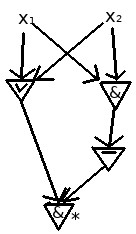
\includegraphics[height=150pt]{27} \quad\quad\quad\quad\quad\quad\quad\quad\quad\quad\quad\quad 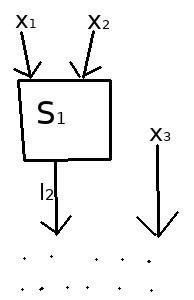
\includegraphics[height=150pt]{28}\\
\subsection{Функция Шеннона для СФЭ.}
	$L(n) = \underset{f(x_1,\dotsc,x_n) \in P_2}{\max}(L(f))$ — ф-я Шеннона
\subsection{Метод Шеннона.}
	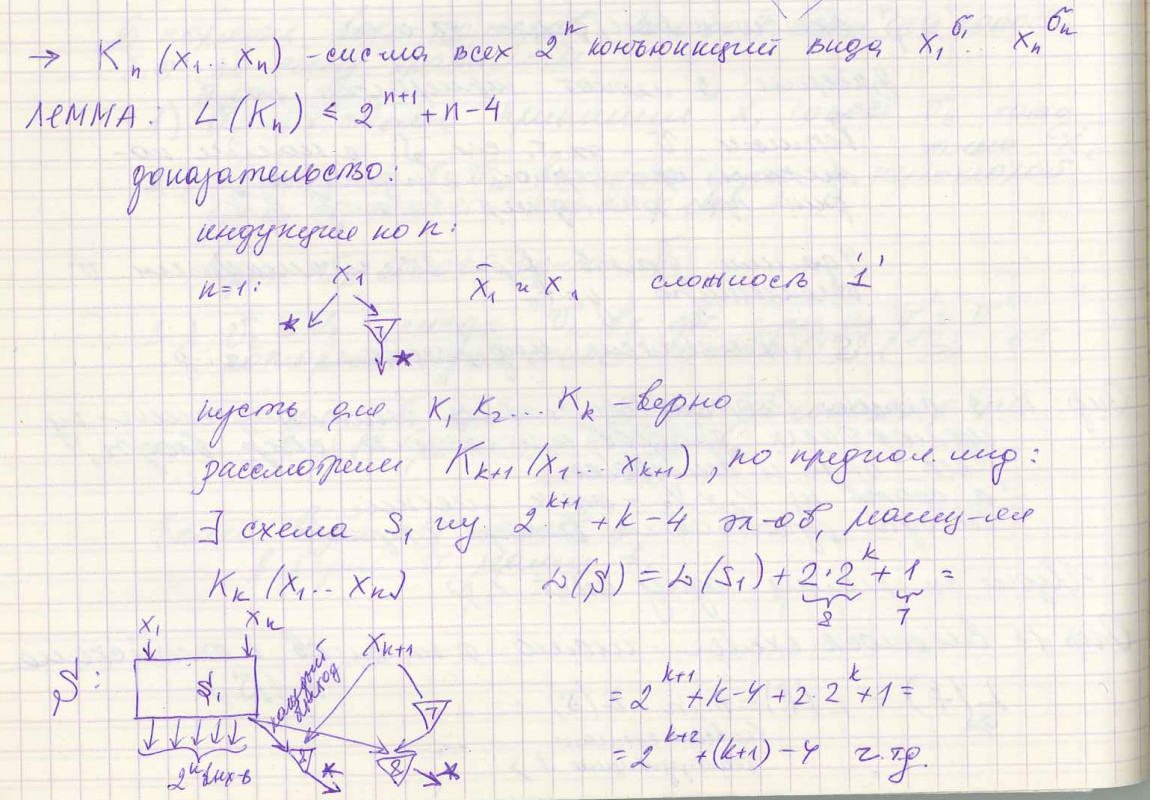
\includegraphics[width=450pt]{29}\\\\
	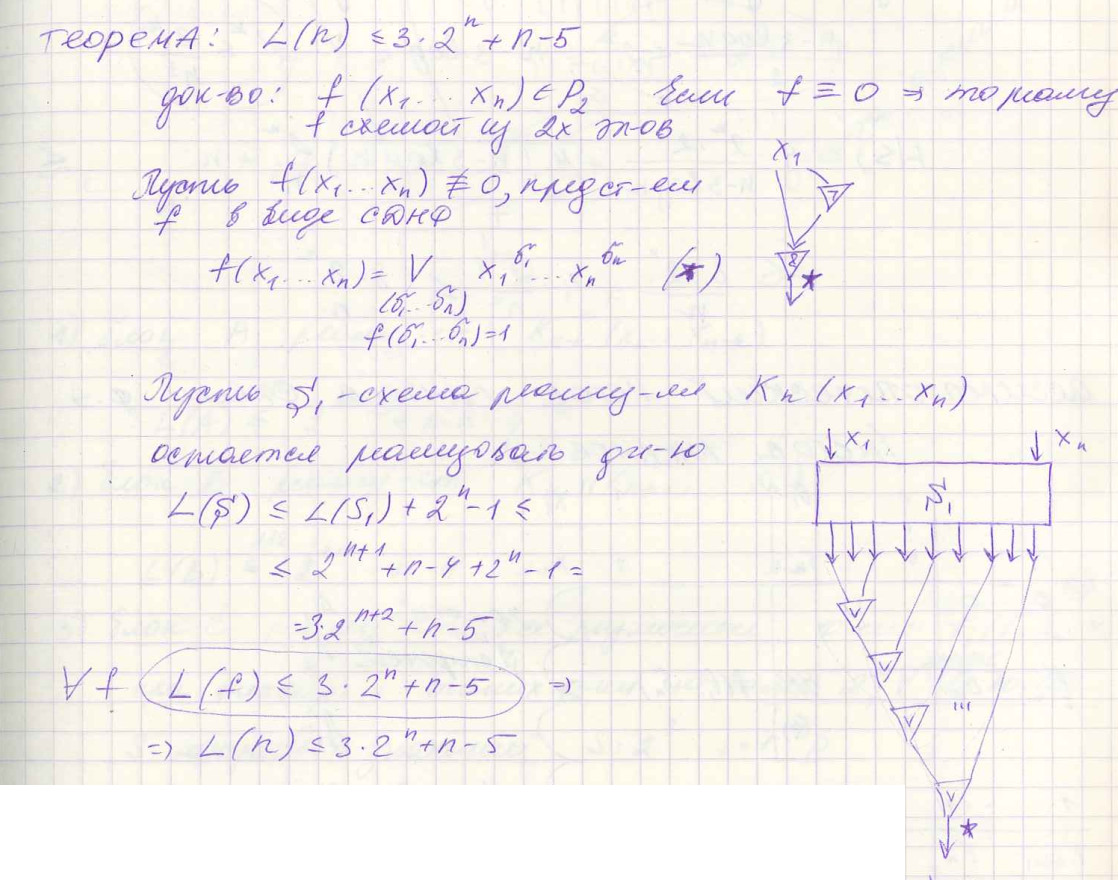
\includegraphics[width=400pt]{30}\\
	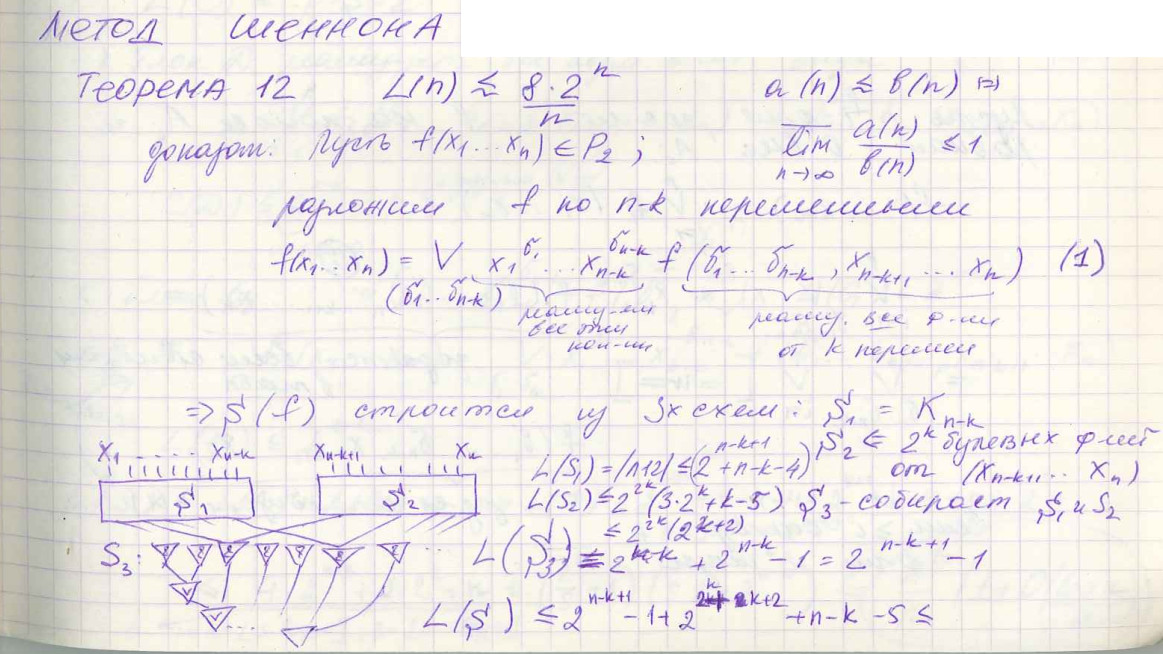
\includegraphics[width=400pt]{31}\\
	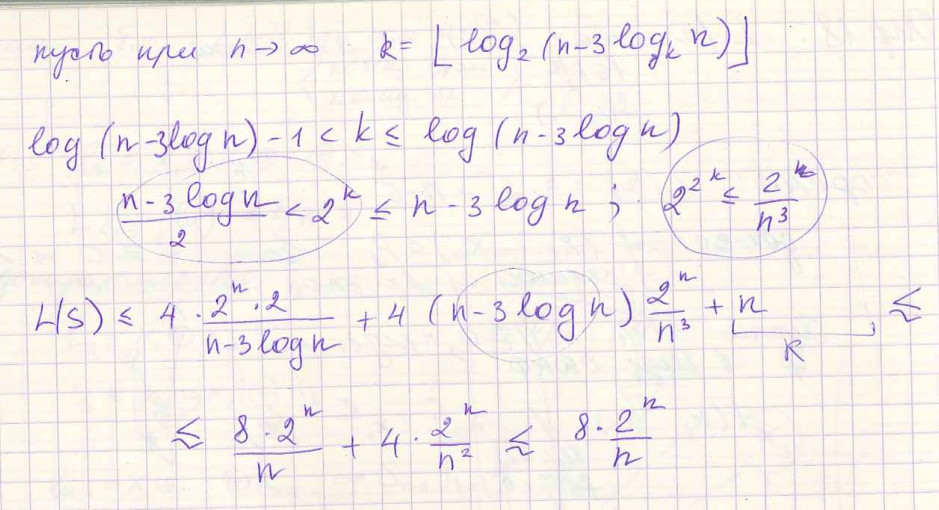
\includegraphics[width=400pt]{32}\\

\section{Лемма о нижней оценке сложности схем.}
	$N(k, n) \leqslant (32(n+k))^{n+k+3}$\\
	\textbf{Доказательство:}\\
		(в доказательстве ниже у функции N аргумены на других местах)\\
		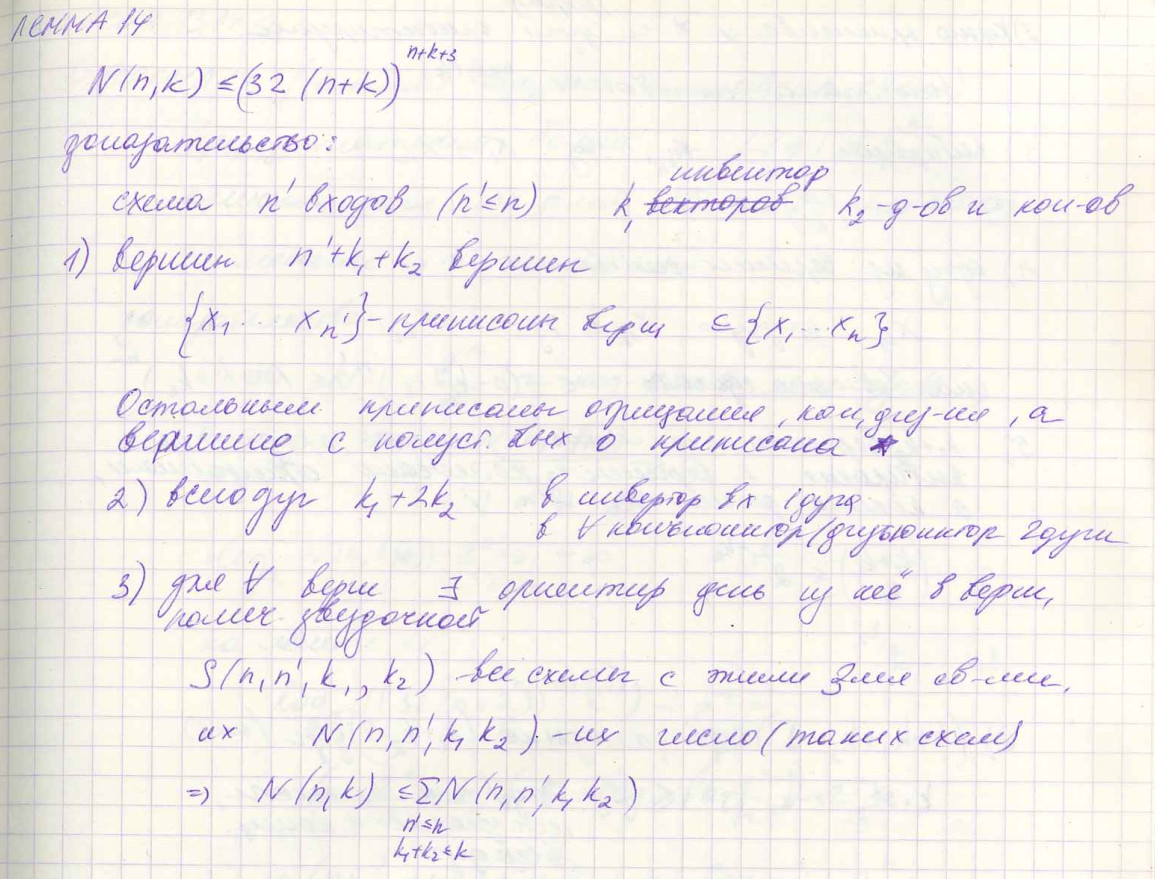
\includegraphics[width=500pt]{33}\\
		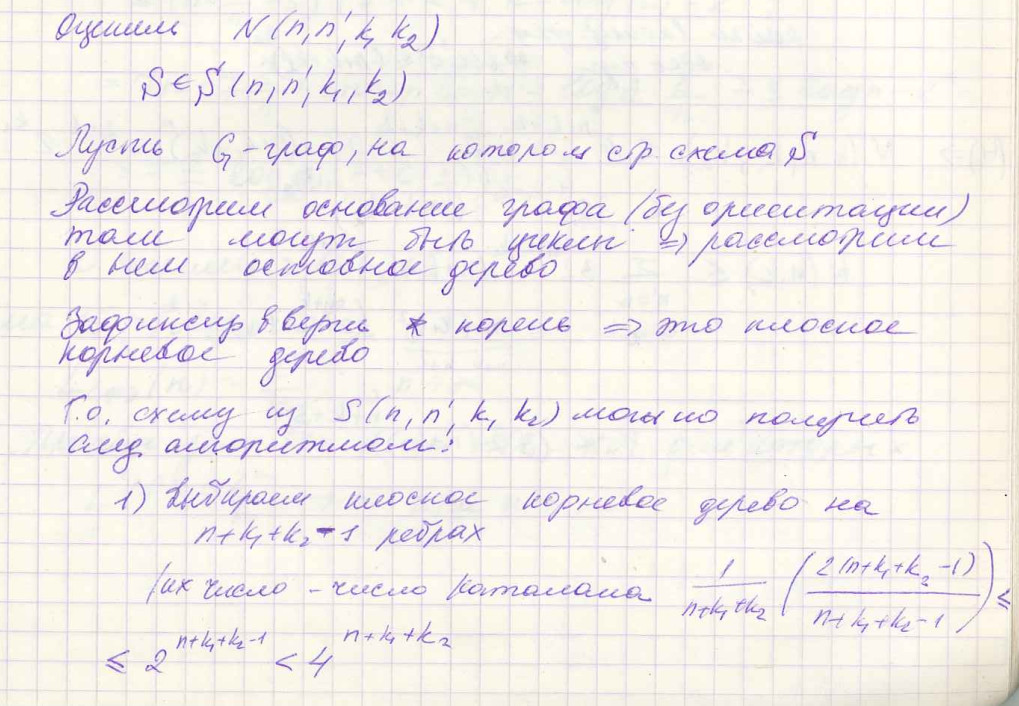
\includegraphics[width=500pt]{34}\\
		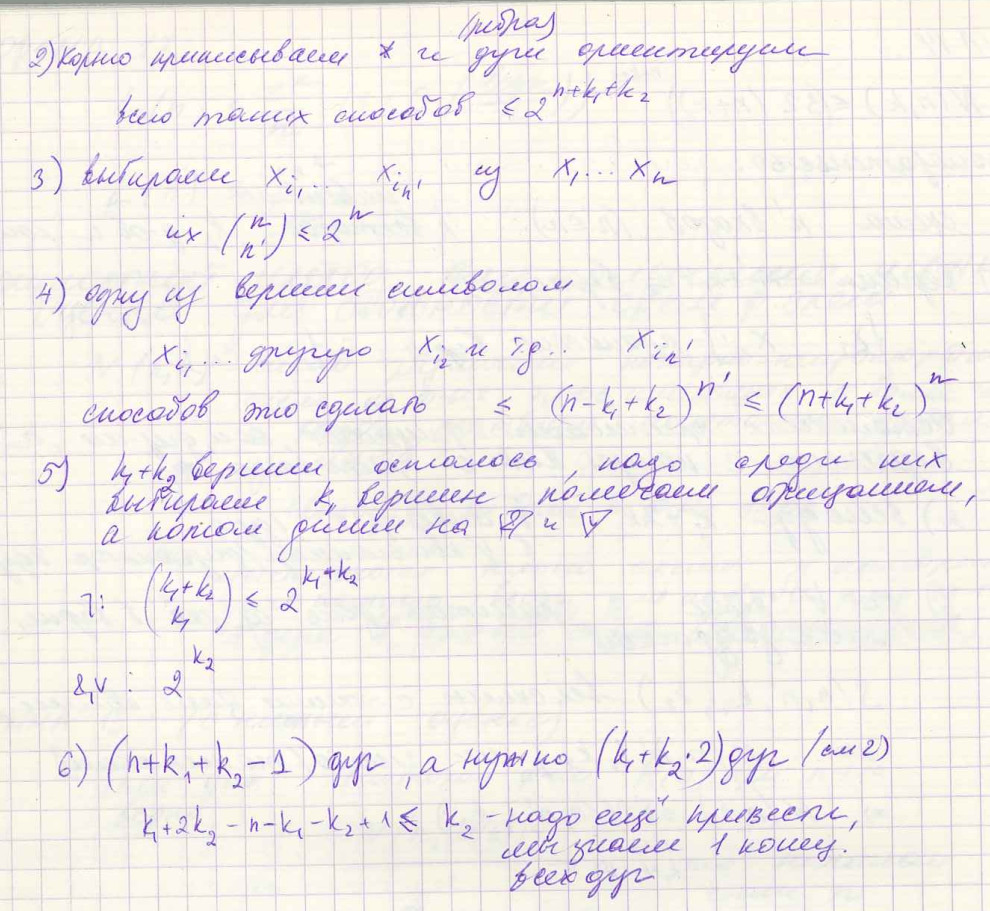
\includegraphics[width=400pt]{35}\\
		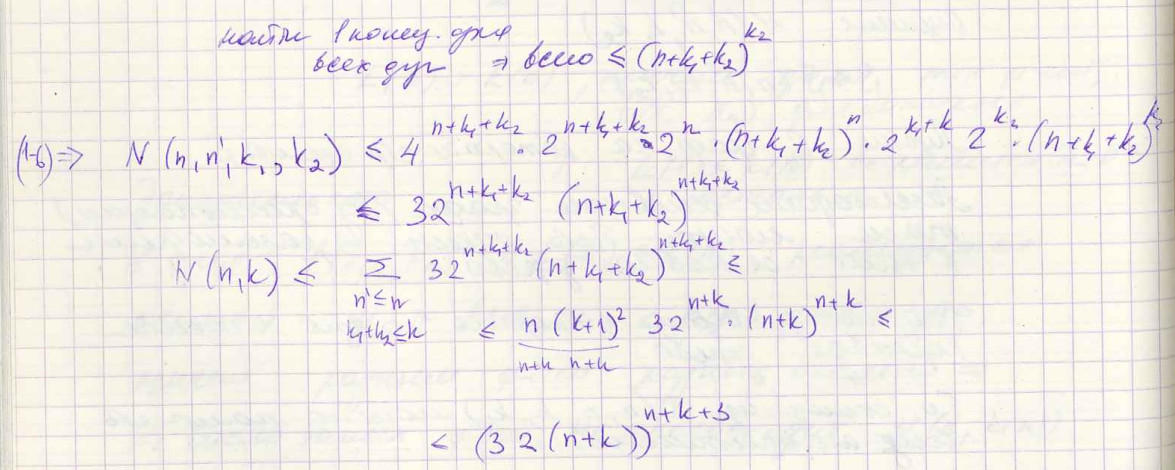
\includegraphics[width=500pt]{36}\\
	\qedsymbol

\section{Мощностной метод получения нижней оценки функции Шеннона для СФЭ}
?\\
	Для достаточно больших $n$\\
	L(n) > $\frac{2^n}{n}$ и доля тех, ф-ций $f(x_1,\dotsc,x_n)$, для которых $L(f) \leqslant \frac{2^n}{n}$ стремится к $0$ при $n \to \infty$\\
	\textbf{Доказательство:}\\
		Надо показать:\\
		$\frac{N(\frac{2^n}{n}, n)}{2^{2^n}} \underset{n \to \infty}{\to} 0$\\
		Из леммы о нижней оценке\\
		$\log_2 N(\frac{2^n}{n}, n) - 2^n \underset{n \to \infty}{\to} 0$\\
		$(n+\frac{2^n}{n}+3)\log_2(32(n+\frac{2^n}{n})) - 2^n \leqslant (n+\frac{2^n}{n}+3)(5 + \log_2(\frac{2^{n+2}}{n})) - 2^n = (n+\frac{2^n}{n}+3)(7 + n - \log_2n) - 2^n = 7n + n^2 - n\log_2n + 7 \cdot \frac{2^n}{n} + 2^n - \frac{2^n}{n} \log_2n + 21 + 3n - 3\log_2n - 2^n \underset{n \to \infty}{\to} -\infty$\\
	\qedsymbol

\section{Ограниченно-детерминированные функции. Способы их задания.}
\subsection{Ограниченно-детерминированные функцииции}
	Информационные деревья эквивалентны, если они задают одинаковую функцию\\
	$f(x)$ — ограниченно детерминированная ф-я, если в её информационном дереве конечное число попарно не эквивалентных поддеревьев
\subsection{Способы их задания.}
\subsubsection{Определение}
	Рассмотрим $f(x)$ — о.д.ф веса $r$; $v_0, \dotsc, v_{r-1: T_{v_0}, \dotsc, T_{v_{r-1}}}$ попарно неэквивалентны\\
	Пометим все вершины дерева $T_{v_0}$ числами $q_0, \dotsc, q_{r-1}$\\
	Т.о. дерево $T_u$ имеет метку $q_j$ $\Leftrightarrow$ $T_u ~ T_{v_j}$
\subsubsection{Определение}
	$\{q_0, \dotsc, q_{r-1}\} = Q$ — мн-во состояний о.д.ф. $f$
\subsubsection{1. Усечённое информационное дерево}
	Усечённое информационное дерево — поддерево $T_{v_0}$ т. ч. $\forall$ орцепь из $v_0$ в лист содержит ровно $2$ вершины с $1$-ой меткойи никакое поддерево этим св-вом не обладает
\subsubsection{2. Диаграмма Мура}
	Отождествим все вершины с одинаковыми метками в усечённом информационном дереве, получим диаграмму о.д.ф.\\
	Также необходимо задать начальную вершину
\subsubsection{3. Канонические уравнения}
	$\delta: Q \times A \to Q$ 	— ф-я переходов\\
	$\lambda: Q \times A \to B$	— ф-я выходов
	\\
	$\begin{cases}
		y(t) = \lambda(q(t), x(t))\\
		q(t+1) = \delta(q(t), x(t))\\
		q(q) = q_0
	\end{cases}$

\section{Конечный детерминированный автомат с выходом. Автоматные функции, связь с ограниченно-детерминированными функциями. Лемма о периодической функции.}
\subsection{Конечный детерминированный автомат с выходом.}
	Он же автомат Мили: система $V = (A, B, Q, \delta, \lambda)$:\\
	$A = \{a_1, \dotsc, a_n\}$ — входной алфавит\\
	$B = \{b_1, \dotsc, b_m\}$ — выходной алфавит\\
	$Q = \{q_1, \dotsc, q_k\}$ — выходной алфавит\\
	$\delta: Q \times A \to Q$ — ф-я переходов\\
	$\lambda: Q \times A \to B$ — ф-я выходов\\
\subsection{Автоматные функции, связь с ограниченно-детерминированными функциями.}
	Ф-я $f: A^{\inf} \to B^{\inf}$ — автоматная, если $\exists$ конечн. детерм. автомат её реализующий\\
	\textbf{Лемма:}\\
		ф-я автоматная $\Leftrightarrow$ она ограниченно детерминированная\\
\subsection{Лемма о периодической функции}
	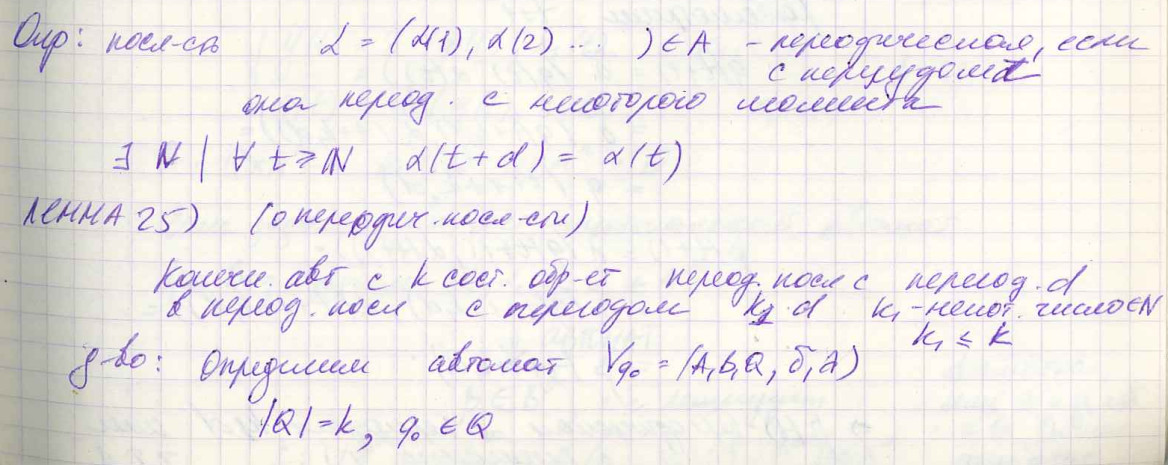
\includegraphics[width=500pt]{37}\\
	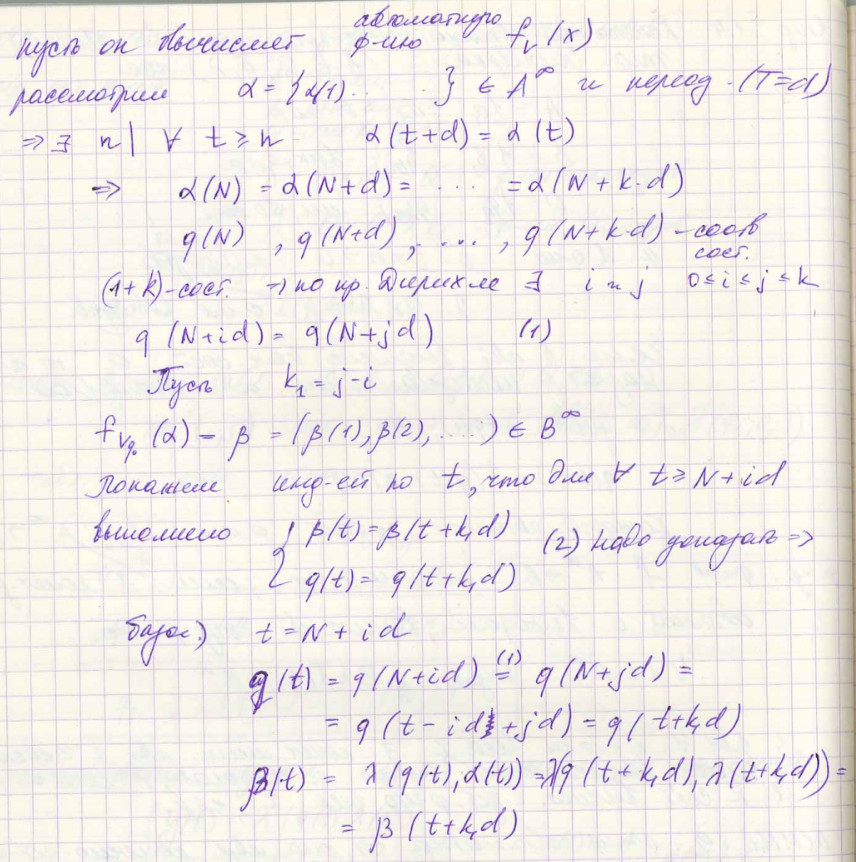
\includegraphics[width=500pt]{38}\\
	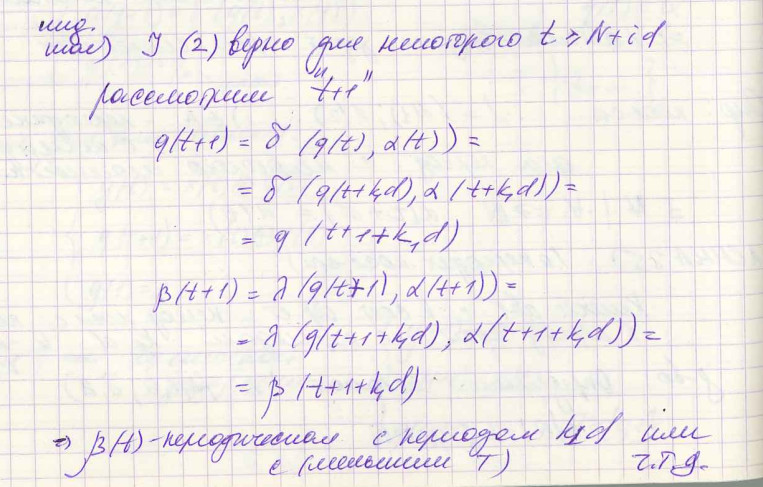
\includegraphics[width=500pt]{39}

\section{Схема из автоматных элементов. Теорема о не существовании конечных полных систем автоматных функций.}
\subsection{Схема из автоматных элементов.}
	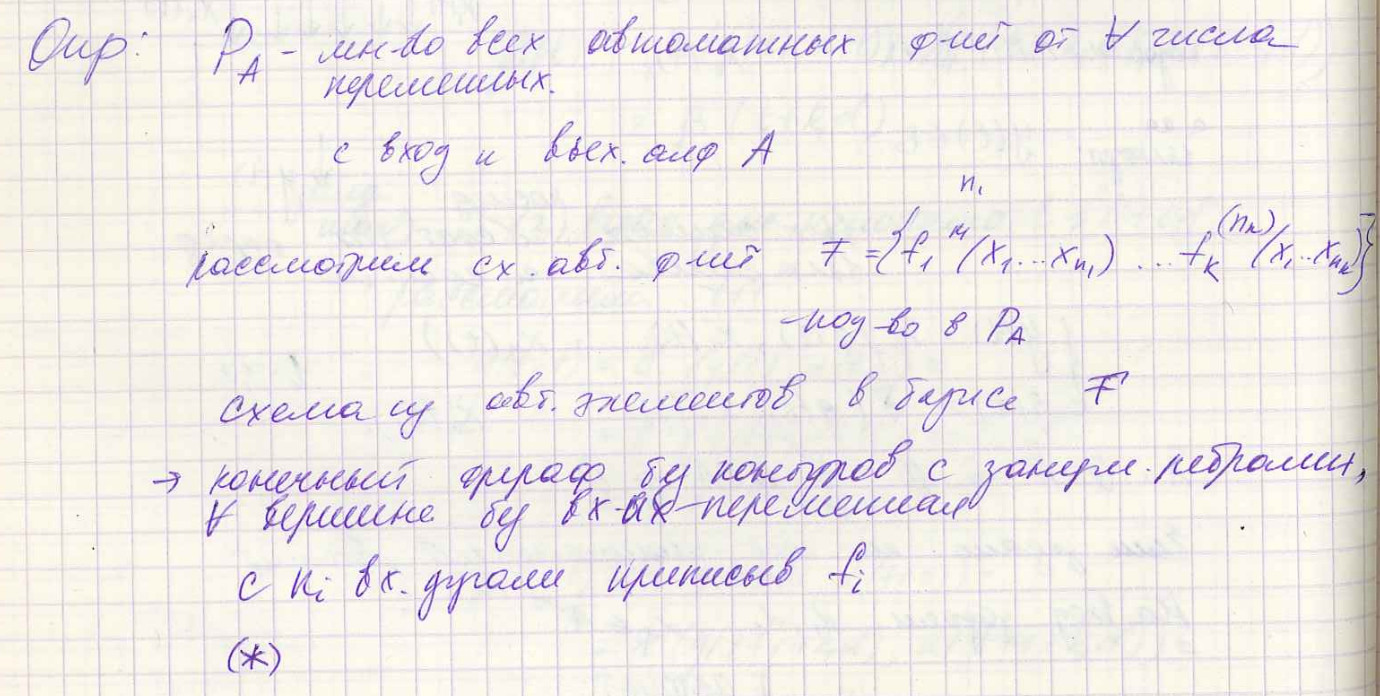
\includegraphics[width=500pt]{44}
\subsection{Теорема о не существовании конечных полных систем автоматных функций.}
	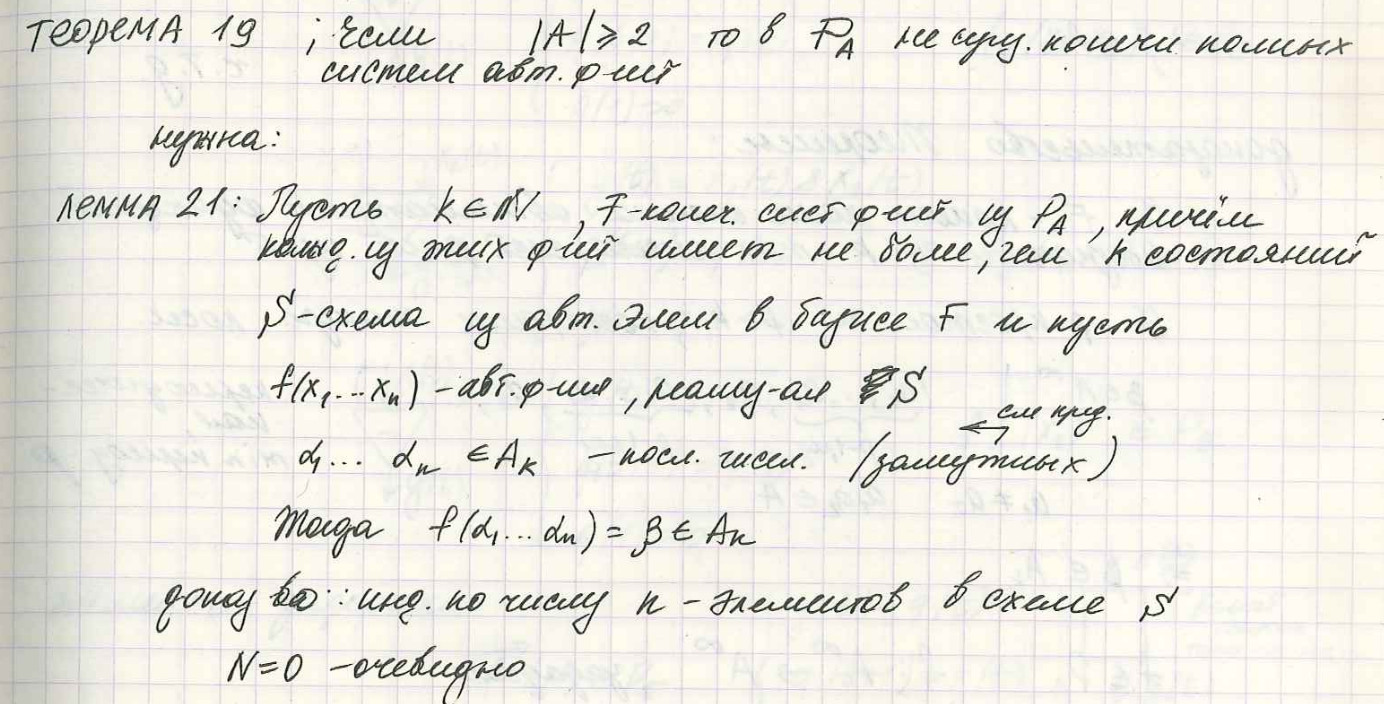
\includegraphics[width=500pt]{40}\\
	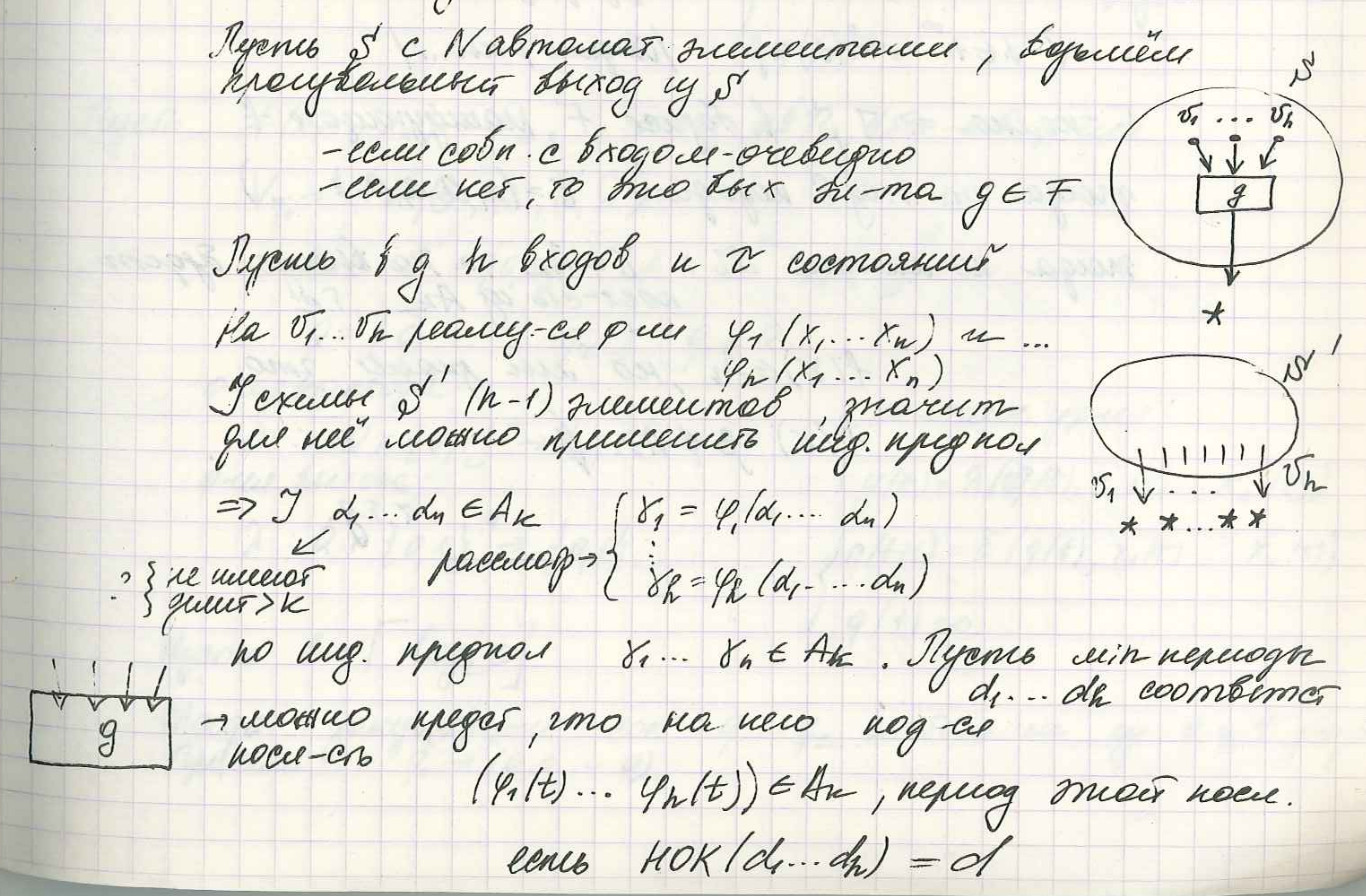
\includegraphics[width=500pt]{41}\\
	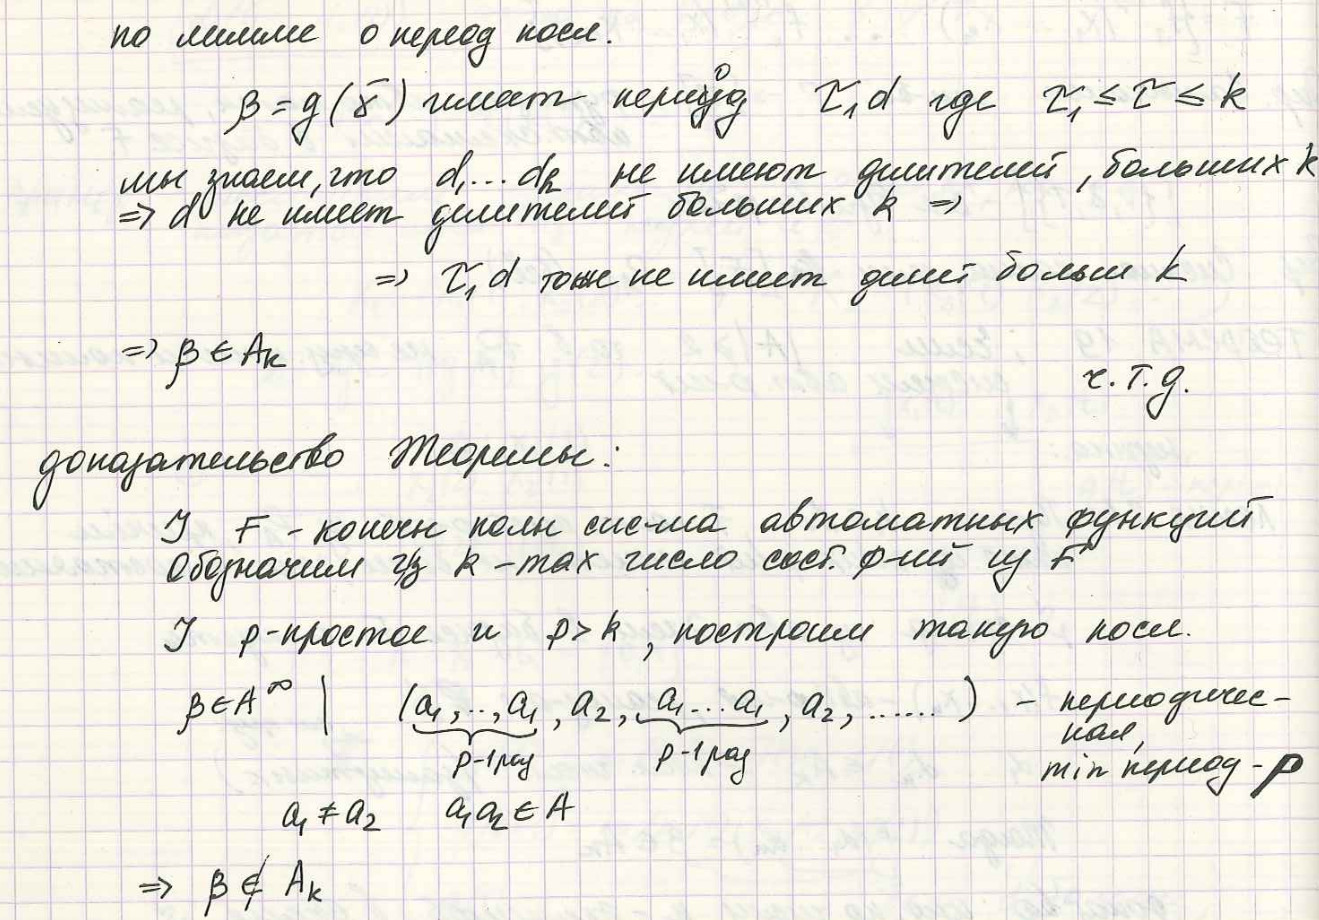
\includegraphics[width=500pt]{42}\\
	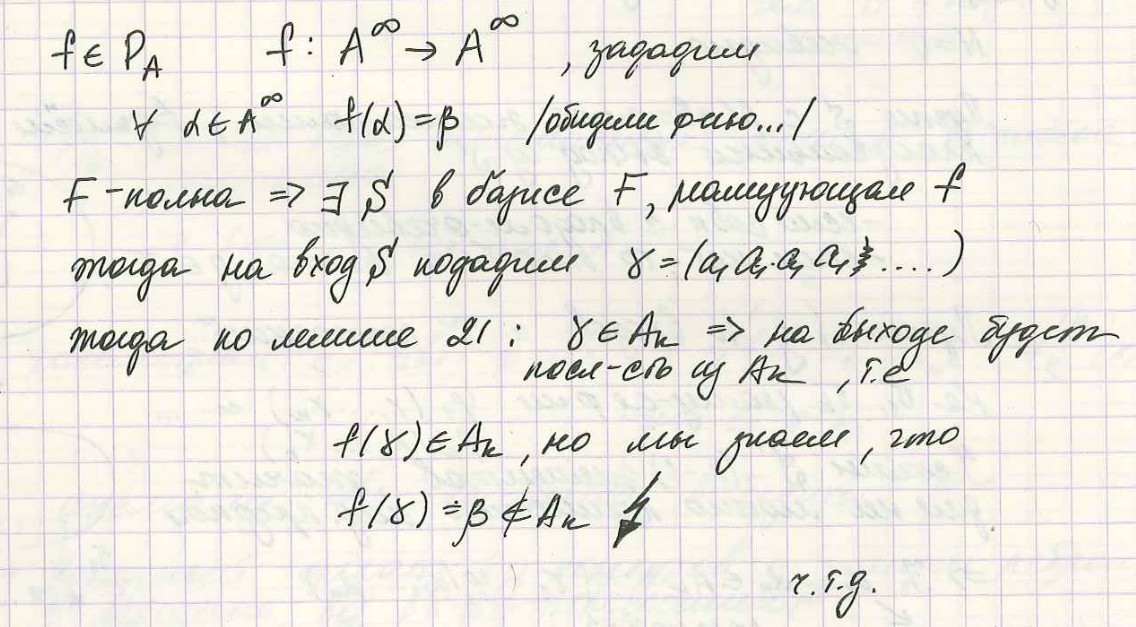
\includegraphics[width=500pt]{43}

\section{Схемы из автоматных элементов с использованием операции обратной связи. Реализация произвольной автоматной функции.}
\subsection{Схемы из автоматных элементов с использованием операции обратной связи.}
	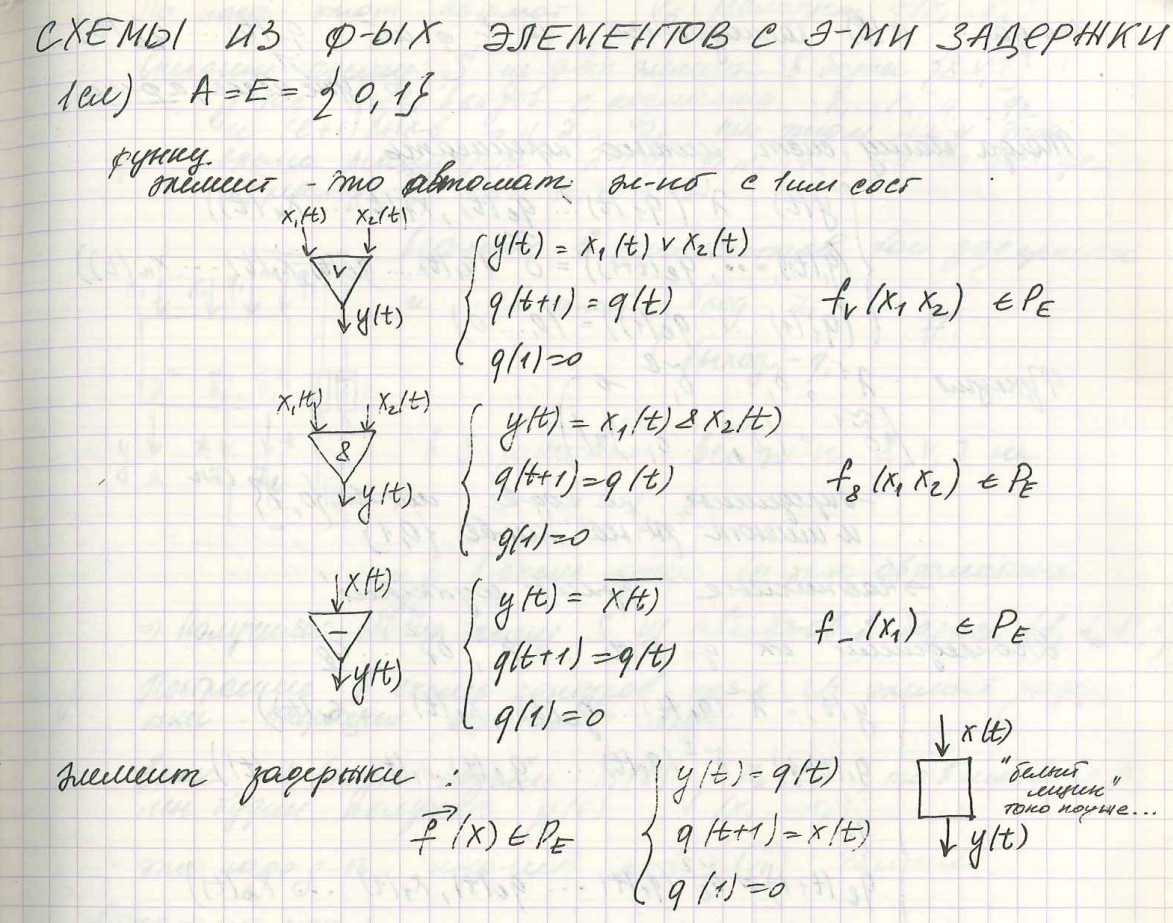
\includegraphics[width=450pt]{45}\\
	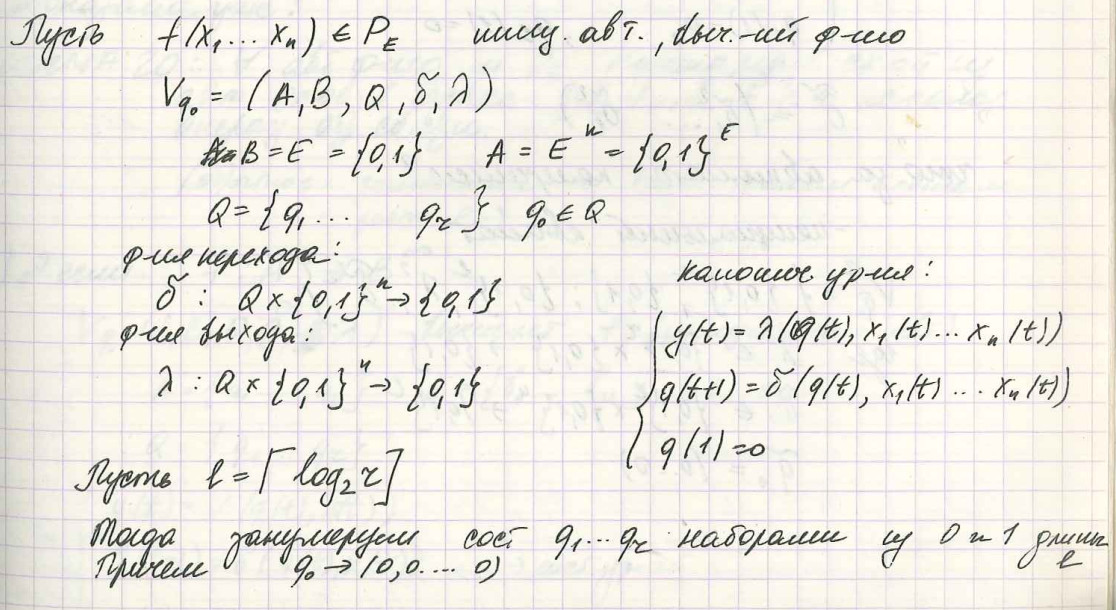
\includegraphics[width=450pt]{46}\\
	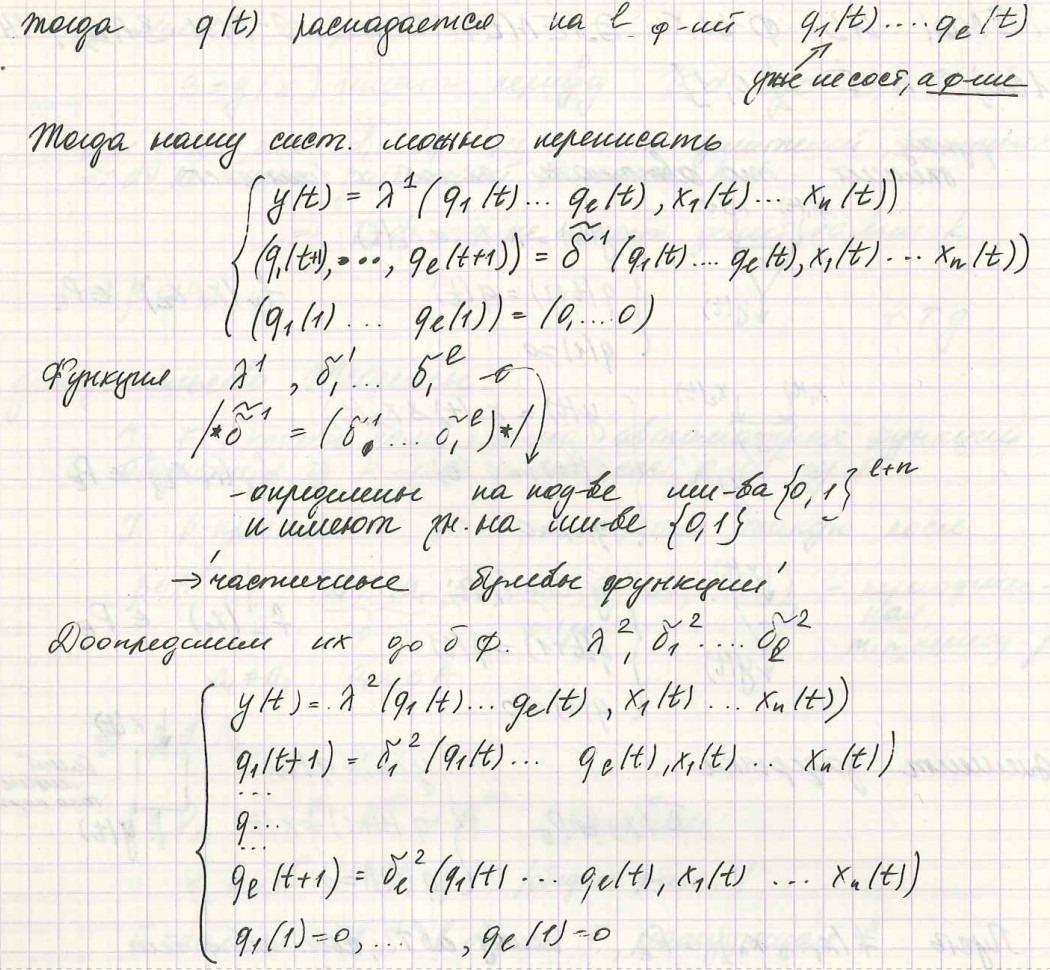
\includegraphics[width=450pt]{47}\\
	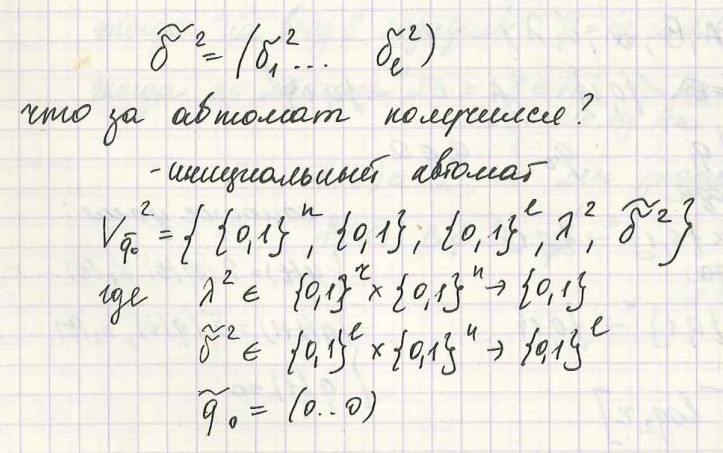
\includegraphics[width=450pt]{48}\\
	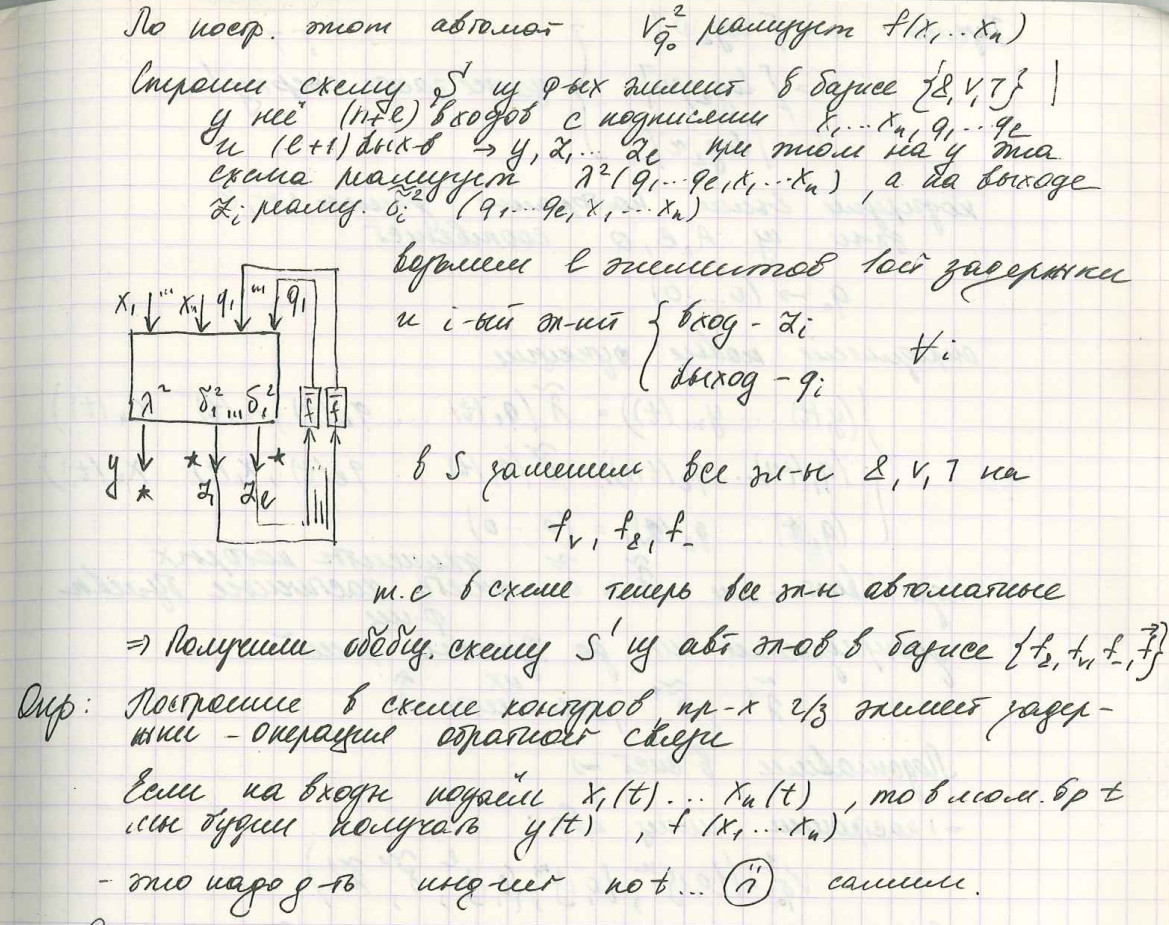
\includegraphics[width=450pt]{49}\\
	\includegraphics[width=450pt]{50}
\subsection{Реализация произвольной автоматной функции.}
	Для $\forall$ автоматной ф-ции $f \in P_A$ можно построить схему из автоматных элементов в базисе ${f_{\&}, f_{\vee}, f_{\bar{}}, \overrightarrow{\mkern -3mu f\mkern 3mu}}$ с использованием операции обр. связи, реализующую систему б.ф. $f_1,\dotsc,f_m \in P_E$ ($m = \lceil \log_2|B| \rceil$) значения которых однозначно опр. значение $f$

\section{Конечные автоматы Мили и Мура, их эквивалентность.}
\subsection{Конечный автоматы Мили}
	Система $V = (A, B, Q, \delta, \lambda)$:\\
	$A = \{a_1, \dotsc, a_n\}$ — входной алфавит\\
	$B = \{b_1, \dotsc, b_m\}$ — выходной алфавит\\
	$Q = \{q_1, \dotsc, q_k\}$ — выходной алфавит\\
	$\delta: Q \times A \to Q$ — ф-я переходов\\
	$\lambda: Q \times A \to B$ — ф-я выходов\\
\subsection{Конечный автомат Мура}
	Конечный детерминированный автомат — автомат Мура, если $\forall$ состояния $q$ значение выходного символа на всех входящих в $q$ дугах одинаково
\subsection{эквивалентность автоматов Мили и Мура}
	$\forall$ автомата Мили, $\exists$ эквивалентный ему автомат Мура\\
	\textbf{Доказательство:}\\
	Дан произвольный автомат Мили: $(A, B, Q, \delta, \lambda)$\\
	$A = (a_1, \dotsc, a_n)$\\
	$Q = (q_1, \dotsc, q_k)$\\
	Определим автомат Мура: $V_M = (A, B, Q_M, \delta_M, \mu)$\\
	$Q_M = \{q_{ij} | i = 1,\dotsc,k; j = 1, \dotsc, n\} \cup \{q_{i0} | i = 1,\dotsc,k\}$\\
	$q_{i0}$ — исх. состояния\\
	$q_{ij} (j > 1)$ — исх. дуги\\
	$\delta_M:$ $\delta_M(q_{i0}, a_r) = q_{ir}; i = 1,\dotsc,k$\\
				$\delta_M(q_{ij}, a_r) = q_{lr}; l: \delta(q_i,a_j) = q_l$\\
	$\mu:$ $\mu(q_{io})$ — произвольные значения\\
	$\mu:$ $\mu(q_{ij}) = \lambda(q_i, a_j)$\\
	Автомат построили, теперь необходимо обосновать:\\
	1) $\forall i = 1, \dotsc, k \quad q_i \in Q$ автомата $V$ неотличимо от $q_{i0} \in Q_M$ автомата $V_M$\\ 
	2) $\forall i = 1, \dotsc, k; \forall j = 1, \dotsc, n \quad q_{ij} \in Q_M$ неотличимо от $q_{r0} \in Q_M\ \quad r: \delta(q_i, a_j) = q_r$\\
	Обоснование:\\
	1) В автомате $V$ при состоянии $q_i$ подадим на вход $a_r$, на выходе получим $\lambda(q_i, a_r)$\\
	В автомате $V_M$ при состоянии $q_{i0}$ подадим на вход $a_r$\\
	$\lambda_M(q_{i0}, a_r) = \mu(\delta_M(q_{io}, a_r)) = \mu(q_{ir}) = \lambda(q_i, a_r)$\\
	2) б/д\\ 
	\qedsymbol

\section{Конечный детерминированный инициальный автомат без выходов. Пример языка, не распознаваемого конечным автоматом.}
\subsection{Конечный детерминированный инициальный автомат без выходов.}
	$V = (A, Q, \delta, q_0, F)$\\
	$A$ — входной алфавит\\
	$Q = \{q_1, \dotsc, q_k\}$ — мн-во состояний\\
	$\delta: Q \times A \to Q$ — ф-я переходов\\
	$q_0$ — нач. состояние\\
	$F \subset Q$ — мн-во конечных состояний
\subsection{Пример языка, не распознаваемого конечным автоматом.}
%	Мн-во всех префиксов бесконечной непериодической последовательности не распознаётся конечным автоматом\\
%	\textbf{Доказательство:}\\
%		$x_1x_2\dotsc$ — беск. непериодич. послед\\
%		$V$ — автомат Мура, распознающий $E = \{x_1,x_1x_2,x_1x_2x_3,\dotsc\}$\\
%		1) $\forall k = 1,\dotsc \quad$ $\delta(q_0, x_1\dotsc x_n) \in F$\\
%		2) $\forall \alpha \quad$ $\delta(q_0, \alpha) \in F \Rightarrow \alpha = x_1\dotsc x_{|\alpha|}$\\
%		Т. к. последовательность непериодическая, то $\exists s, j:$ $\delta(q_0, x_1\dotsc x_j) = \delta(q_0, x_1 \dotsc x_{j + s}) $
%	\qedsymbol
	\includegraphics[width=500pt]{51}\\
	\includegraphics[width=500pt]{52}

\section{Конечные автоматы без выходов. Регулярные языки. Теорема о детерминизации.}
\subsection{Конечные автоматы без выходов.}
\subsubsection{Конечный детерминированный инициальный автомат без выходов}
	$V = (A, Q, \delta, q_0, F)$\\
	$A$ — входной алфавит\\
	$Q = \{q_1, \dotsc, q_k\}$ — мн-во состояний\\
	$\delta: Q \times A \to Q$ — ф-я переходов\\
	$q_0$ — нач. состояние\\
	$F \subset Q$ — мн-во конечных состояний
\subsubsection{Конечный недетерминированный автомат без выходов}
	$V = (A, Q, \delta, q_0, F)$\\
	$\delta: Q \times (A \cup \{e\}) \to 2^Q$\\
	$2^Q = \{S | S \subseteq Q\}$ — множество всех подмножеств $Q$
\subsection{Регулярные языки.}
	\begin{enumerate}
		\item $E_1 + E_2 = E_1 \cup E_2$ — объединение
		\item $E_1 \cdot E_2 = \{\alpha_1\alpha_2 | \alpha_1 \in E_1; \alpha_2 \in E_2\}$ — конкатенация
		\item $E^* = \{e\} \cup E \cup E^2 \cup \dotsc = \displaystyle\bigcup_{i=0}^\infty E^i$ — итерация
	\end{enumerate}
	$A = \{a_1, \dotsc, a_n\}$\\
	языки $\{e\}, \{a_1\}, \dotsc, \{a_n\}$ — элементарные языки\\

	Язык $E \subseteq A^*$ — регулярный, если он может быть получен из элементарных языков конечным числом операций объединения, конкатенации и итерации\\

\subsection{Теорема о детерминизации.}
	Введём подобные обозначения\\
	\includegraphics[width=400pt]{53}\\
	\includegraphics[width=400pt]{54}\\
	\includegraphics[width=400pt]{55}\\
	\includegraphics[width=400pt]{56}\\
	\includegraphics[width=400pt]{57}

\section{Конечные автоматы без выходов. Регулярные языки. Теорема анализа автоматов}
\subsection{Конечные автоматы без выходов.}
	См. пункт 64.1
\subsection{Регулярные языки.}
	См. пункт 64.2
\subsection{Теорема анализа автоматов}
	$Событие = слово$\\
	\includegraphics[width=550pt]{61}\\
	\includegraphics[width=550pt]{62}
	\qedsymbol

\section{Конечные автоматы без выходов. Регулярные языки. Теорема синтеза автоматов}
\subsection{Конечные автоматы без выходов.}
	См. пункт 64.1
\subsection{Регулярные языки.}
	См. пункт 64.2
\subsection{Теорема, необходимая для доказательства}
	$\forall$ регулярного языка $\exists$ недетерминированный конечный автомат с одним закл. состоянием распознающий его\\
	\textbf{Доказательство:}\\
	База: элементарный язык\\

	Операции:\\
	$E_1, E_2$ — языки, распознаваемые автоматом с одним закл. сост.\\
	\includegraphics[width=300pt]{58}\\
	\includegraphics[width=400pt]{59}\\
	\includegraphics[width=400pt]{60}\\
\subsection{Теорема синтеза автоматов}
	$\forall$ регулярного языка $E$ существует конечный автомат, распознающий этот язык\\
	\textbf{Доказательство:}\\
		Для регулярного языка $E$ строим недетерминированный конечный автомат по доказанной выше теореме\\
		Строим для полученного автомата эквивалентный ему детерминированный конечный автомат (по теореме о детерминизации)\\
	\qedsymbol

\section{Классы P и NP. Полиномиальная сводимость. NP-полные задачи. Теорема Кука (без доказательства)}
\subsection{Классы P и NP.}
	$L[П, \varepsilon]$ — {коды задач из $Y_П$}\\
	$П \in P$ — $\exists$ полиномиальный алгоритм её распознающий $\Leftrightarrow$ $\exists$ детерминированная машина Тьюринга распознающая $L[П, \varepsilon]$\\\\
	$П \in NP \Leftrightarrow$ $\exists$ недетерм. машина Тьюринга распознающая $L[П, \varepsilon]$ $\Leftrightarrow$ за полиномиальное время можно проверить ответ "да"\\\\
	$P \subseteq NP$\\
\subsection{Полиномиальная сводимость.}
	Задача $П_1$полиномиально сводится к задаче $П_2$ $(П_1 \propto П_2)$, если $\exists$ ф-я $f: D_{П_1} \to D_{П_2}$ т.ч.:
	\begin{enumerate}
		\item $\exists$ полиномиальный алгоритм $A$ вычисляющий $f$
		\item $I \in Y_{П_1} \Leftrightarrow f(П_1) \in Y_{П_2}$
	\end{enumerate}
\subsection{Теорема Кука (без доказательства)}
	Задача ВЫП(выполнимость) NP-полная

\section{Полиномиальная сводимость. Доказательство NP-полноты задачи 3-выполнимость.}
\subsection{Полиномиальная сводимость.}
	Задача $П_1$полиномиально сводится к задаче $П_2$ $(П_1 \propto П_2)$, если $\exists$ ф-я $f: D_{П_1} \to D_{П_2}$ т.ч.:
	\begin{enumerate}
		\item $\exists$ полиномиальный алгоритм $A$ вычисляющий $f$
		\item $I \in Y_{П_1} \Leftrightarrow f(П_1) \in Y_{П_2}$
	\end{enumerate}
\subsection{Доказательство NP-полноты задачи 3-выполнимость.}
	3-выполнимость — NP-полная\\
	\textbf{Доказательство:}
		По теореме Кука задача ВЫП — NP-полная\\
		Также по лемме с лекций:\\
		$П_1, П_2 \in NP, П_1 \in NPC$\\
		$П_1 \propto П_2 \Rightarrow П_2 \in NPC$\\
		$П_1$ — выполнимость\\
		$П_2$ — 3-выполнимость\\
		Т.о. необходимо доказать что 3-выполнимость $\in NP$. И что выполнимость сводится к 3-выполнимости\\
		Обозначения:\\
		3SAT — 3-выполнимость\\
		CNFSAT — выполнимость\\
		\includegraphics[width=580pt]{63}
	\qedsymbol

\section{Полиномиальная сводимость. Доказательство NP-полноты задачи о раскраске.}
\subsection{Полиномиальная сводимость.}
	Задача $П_1$полиномиально сводится к задаче $П_2$ $(П_1 \propto П_2)$, если $\exists$ ф-я $f: D_{П_1} \to D_{П_2}$ т.ч.:
	\begin{enumerate}
		\item $\exists$ полиномиальный алгоритм $A$ вычисляющий $f$
		\item $I \in Y_{П_1} \Leftrightarrow f(П_1) \in Y_{П_2}$
	\end{enumerate}
\subsection{Доказательство NP-полноты задачи о раскраске.}
	Задача Раскраска — NP-полная\\\\
	Дан граф $G$ и дано число $\chi \in Z^+$ $\exists$ ли правильная вершинная раскраска в $\chi цветов$?\\
	\textbf{Доказательство:}\\
		3-ВЫП $\propto$ раскр.\\
		$K = D_1 \& \dotsb \& D_s$ — КНФ над $\{x_1, \dotsc x_n\}$\\
		$\chi = n + 1$\\
		$G: V = \{x_1, \overline{x_1}, x_2, \overline{x_2}, \dotsc, x_n, \overline{x_n}, c_0, \dotsc, c_n, D_1, \dotsc, D_s\}$\\
		$EG = E_1 \cup \dotsb \cup E_5$\\
		$E_1 = \{c_ic_j | \forall i \neq j\}$\\
		$E_2 = \{x_i\overline{x_i} \forall i\}$\\
		$E_3 = \{x_ic_j, \overline{x_i}c_j | j \neq i, j \neq 0\}$\\
		$E_4 = \{D_ju_i, D_ju_k, D_ju_l | D_j = u_i \vee u_k \vee u_l\}$\\
		$E_5 = \{D_jc_p | D_j = u_i \vee u_k \vee u_l; p \notin \{i, k, l\}\}$\\
		Пример:\\
		\includegraphics[height=330pt]{64}\\
		Пусть дан вектор значений $(x_1^*, \dotsc, x_n^*)$ на котором истинна КНФ\\
		Вершины $c_i$ красим в цвет $c_i$\\
		Если $x_i^* = 1$, то окрашиваем вершину $x_i$ в $c_0$, а вершину $\overline{x_i}$ в $c_i$\\
		Если $x_i^* = 0$, то окрашиваем вершину $\overline{x_i}$ в $c_0$, а вершину $x_i$ в $c_i$\\
		Т.к. КНФ истинна, то $\forall D_i \exists x_j^*$ за счёт которой $D_i$ истинна $\Rightarrow$ $\exists$ вершина соединённая с $D_i$  и окрашенная в цвет $c_0$. Красим $D_i$ в цвет $c_j$\\\\
		Пусть дана раскраска графа $G$ строим по этой раскраске вектор значений на котором КНФ будет истинна\\
		$\forall i$ одна из вершин $x_i, \overline{x_i}$ окрашена в цвет $c_0$, а другая в цвет $c_i$. Если в цвет $c_0$ окрашена вершина $x_i$, то на $i$-ом месте в векторе стоит $1$. Если же в цвет $c_0$ окрашена вершина $\overline{x_i}$, то на $i$-ом месте стоит $0$\\
		Понятно что для каждой вершины $D_j \exists$ вершина $x_k$ или $\overline{x_k}$ которая окрашена в цвет $c_0$ (иначе $D_j$ не во что было бы покрасить). И за счёт переменной, которая покрашена в $c_0$, элементарная дизъюнкция $D_j$ становится истинной\\
	\qedsymbol
\end{document}
